\documentclass[twoside]{book}

% Packages required by doxygen
\usepackage{fixltx2e}
\usepackage{calc}
\usepackage{doxygen}
\usepackage[export]{adjustbox} % also loads graphicx
\usepackage{graphicx}
\usepackage[utf8]{inputenc}
\usepackage{makeidx}
\usepackage{multicol}
\usepackage{multirow}
\PassOptionsToPackage{warn}{textcomp}
\usepackage{textcomp}
\usepackage[nointegrals]{wasysym}
\usepackage[table]{xcolor}

% Font selection
\usepackage[T1]{fontenc}
\usepackage[scaled=.90]{helvet}
\usepackage{courier}
\usepackage{amssymb}
\usepackage{sectsty}
\renewcommand{\familydefault}{\sfdefault}
\allsectionsfont{%
  \fontseries{bc}\selectfont%
  \color{darkgray}%
}
\renewcommand{\DoxyLabelFont}{%
  \fontseries{bc}\selectfont%
  \color{darkgray}%
}
\newcommand{\+}{\discretionary{\mbox{\scriptsize$\hookleftarrow$}}{}{}}

% Page & text layout
\usepackage{geometry}
\geometry{%
  a4paper,%
  top=2.5cm,%
  bottom=2.5cm,%
  left=2.5cm,%
  right=2.5cm%
}
\tolerance=750
\hfuzz=15pt
\hbadness=750
\setlength{\emergencystretch}{15pt}
\setlength{\parindent}{0cm}
\setlength{\parskip}{3ex plus 2ex minus 2ex}
\makeatletter
\renewcommand{\paragraph}{%
  \@startsection{paragraph}{4}{0ex}{-1.0ex}{1.0ex}{%
    \normalfont\normalsize\bfseries\SS@parafont%
  }%
}
\renewcommand{\subparagraph}{%
  \@startsection{subparagraph}{5}{0ex}{-1.0ex}{1.0ex}{%
    \normalfont\normalsize\bfseries\SS@subparafont%
  }%
}
\makeatother

% Headers & footers
\usepackage{fancyhdr}
\pagestyle{fancyplain}
\fancyhead[LE]{\fancyplain{}{\bfseries\thepage}}
\fancyhead[CE]{\fancyplain{}{}}
\fancyhead[RE]{\fancyplain{}{\bfseries\leftmark}}
\fancyhead[LO]{\fancyplain{}{\bfseries\rightmark}}
\fancyhead[CO]{\fancyplain{}{}}
\fancyhead[RO]{\fancyplain{}{\bfseries\thepage}}
\fancyfoot[LE]{\fancyplain{}{}}
\fancyfoot[CE]{\fancyplain{}{}}
\fancyfoot[RE]{\fancyplain{}{\bfseries\scriptsize Generated by Doxygen }}
\fancyfoot[LO]{\fancyplain{}{\bfseries\scriptsize Generated by Doxygen }}
\fancyfoot[CO]{\fancyplain{}{}}
\fancyfoot[RO]{\fancyplain{}{}}
\renewcommand{\footrulewidth}{0.4pt}
\renewcommand{\chaptermark}[1]{%
  \markboth{#1}{}%
}
\renewcommand{\sectionmark}[1]{%
  \markright{\thesection\ #1}%
}

% Indices & bibliography
\usepackage{natbib}
\usepackage[titles]{tocloft}
\setcounter{tocdepth}{3}
\setcounter{secnumdepth}{5}
\makeindex

% Hyperlinks (required, but should be loaded last)
\usepackage{ifpdf}
\ifpdf
  \usepackage[pdftex,pagebackref=true]{hyperref}
\else
  \usepackage[ps2pdf,pagebackref=true]{hyperref}
\fi
\hypersetup{%
  colorlinks=true,%
  linkcolor=blue,%
  citecolor=blue,%
  unicode%
}

% Custom commands
\newcommand{\clearemptydoublepage}{%
  \newpage{\pagestyle{empty}\cleardoublepage}%
}

\usepackage{caption}
\captionsetup{labelsep=space,justification=centering,font={bf},singlelinecheck=off,skip=4pt,position=top}

%===== C O N T E N T S =====

\begin{document}

% Titlepage & ToC
\hypersetup{pageanchor=false,
             bookmarksnumbered=true,
             pdfencoding=unicode
            }
\pagenumbering{alph}
\begin{titlepage}
\vspace*{7cm}
\begin{center}%
{\Large Trabalho T\+P2 }\\
\vspace*{1cm}
{\large Generated by Doxygen 1.8.13}\\
\end{center}
\end{titlepage}
\clearemptydoublepage
\pagenumbering{roman}
\tableofcontents
\clearemptydoublepage
\pagenumbering{arabic}
\hypersetup{pageanchor=true}

%--- Begin generated contents ---
\chapter{Hierarchical Index}
\section{Class Hierarchy}
This inheritance list is sorted roughly, but not completely, alphabetically\+:\begin{DoxyCompactList}
\item \contentsline{section}{Controller\+Init}{\pageref{class_controller_init}}{}
\item \contentsline{section}{Interface\+B\+L\+Admin}{\pageref{class_interface_b_l_admin}}{}
\begin{DoxyCompactList}
\item \contentsline{section}{Controller\+B\+L\+Admin}{\pageref{class_controller_b_l_admin}}{}
\end{DoxyCompactList}
\item \contentsline{section}{Interface\+B\+L\+Auth}{\pageref{class_interface_b_l_auth}}{}
\begin{DoxyCompactList}
\item \contentsline{section}{Controller\+B\+L\+Auth}{\pageref{class_controller_b_l_auth}}{}
\end{DoxyCompactList}
\item \contentsline{section}{Interface\+B\+L\+Quiz}{\pageref{class_interface_b_l_quiz}}{}
\begin{DoxyCompactList}
\item \contentsline{section}{Controller\+B\+L\+Quiz}{\pageref{class_controller_b_l_quiz}}{}
\end{DoxyCompactList}
\item \contentsline{section}{Interface\+B\+L\+User}{\pageref{class_interface_b_l_user}}{}
\begin{DoxyCompactList}
\item \contentsline{section}{Controller\+B\+L\+User}{\pageref{class_controller_b_l_user}}{}
\end{DoxyCompactList}
\item \contentsline{section}{Interface\+U\+I\+Admin}{\pageref{class_interface_u_i_admin}}{}
\begin{DoxyCompactList}
\item \contentsline{section}{Controller\+U\+I\+Admin}{\pageref{class_controller_u_i_admin}}{}
\end{DoxyCompactList}
\item \contentsline{section}{Interface\+U\+I\+Auth}{\pageref{class_interface_u_i_auth}}{}
\begin{DoxyCompactList}
\item \contentsline{section}{Controller\+U\+I\+Auth}{\pageref{class_controller_u_i_auth}}{}
\end{DoxyCompactList}
\item \contentsline{section}{Interface\+U\+I\+Quiz}{\pageref{class_interface_u_i_quiz}}{}
\begin{DoxyCompactList}
\item \contentsline{section}{Controller\+U\+I\+Quiz}{\pageref{class_controller_u_i_quiz}}{}
\end{DoxyCompactList}
\item \contentsline{section}{Interface\+U\+I\+User}{\pageref{class_interface_u_i_user}}{}
\begin{DoxyCompactList}
\item \contentsline{section}{Controller\+U\+I\+User}{\pageref{class_controller_u_i_user}}{}
\end{DoxyCompactList}
\item \contentsline{section}{Question}{\pageref{class_question}}{}
\item \contentsline{section}{Quiz}{\pageref{class_quiz}}{}
\item \contentsline{section}{Stub\+PR}{\pageref{class_stub_p_r}}{}
\item \contentsline{section}{Subject}{\pageref{class_subject}}{}
\item \contentsline{section}{Topic}{\pageref{class_topic}}{}
\item \contentsline{section}{User}{\pageref{class_user}}{}
\end{DoxyCompactList}

\chapter{Class Index}
\section{Class List}
Here are the classes, structs, unions and interfaces with brief descriptions\+:\begin{DoxyCompactList}
\item\contentsline{section}{\hyperlink{class_controller_b_l_admin}{Controller\+B\+L\+Admin} }{\pageref{class_controller_b_l_admin}}{}
\item\contentsline{section}{\hyperlink{class_controller_b_l_auth}{Controller\+B\+L\+Auth} }{\pageref{class_controller_b_l_auth}}{}
\item\contentsline{section}{\hyperlink{class_controller_b_l_quiz}{Controller\+B\+L\+Quiz} }{\pageref{class_controller_b_l_quiz}}{}
\item\contentsline{section}{\hyperlink{class_controller_b_l_user}{Controller\+B\+L\+User} }{\pageref{class_controller_b_l_user}}{}
\item\contentsline{section}{\hyperlink{class_controller_init}{Controller\+Init} \\*Modulo dos controladores }{\pageref{class_controller_init}}{}
\item\contentsline{section}{\hyperlink{class_controller_u_i_admin}{Controller\+U\+I\+Admin} \\*A\+D\+M\+IN }{\pageref{class_controller_u_i_admin}}{}
\item\contentsline{section}{\hyperlink{class_controller_u_i_auth}{Controller\+U\+I\+Auth} \\*A\+U\+T\+H\+E\+N\+T\+I\+C\+A\+T\+I\+ON }{\pageref{class_controller_u_i_auth}}{}
\item\contentsline{section}{\hyperlink{class_controller_u_i_quiz}{Controller\+U\+I\+Quiz} \\*\hyperlink{class_quiz}{Quiz} }{\pageref{class_controller_u_i_quiz}}{}
\item\contentsline{section}{\hyperlink{class_controller_u_i_user}{Controller\+U\+I\+User} \\*U\+S\+ER }{\pageref{class_controller_u_i_user}}{}
\item\contentsline{section}{\hyperlink{class_interface_b_l_admin}{Interface\+B\+L\+Admin} \\*Interface do Modulo BL de Admin }{\pageref{class_interface_b_l_admin}}{}
\item\contentsline{section}{\hyperlink{class_interface_b_l_auth}{Interface\+B\+L\+Auth} \\*Interface do Modulo BL de Autenticacao }{\pageref{class_interface_b_l_auth}}{}
\item\contentsline{section}{\hyperlink{class_interface_b_l_quiz}{Interface\+B\+L\+Quiz} \\*Interface do Modulo BL de \hyperlink{class_quiz}{Quiz} }{\pageref{class_interface_b_l_quiz}}{}
\item\contentsline{section}{\hyperlink{class_interface_b_l_user}{Interface\+B\+L\+User} \\*Interface do Modulo BL de Usuario }{\pageref{class_interface_b_l_user}}{}
\item\contentsline{section}{\hyperlink{class_interface_u_i_admin}{Interface\+U\+I\+Admin} \\*Interface do Modulo UI de Admin }{\pageref{class_interface_u_i_admin}}{}
\item\contentsline{section}{\hyperlink{class_interface_u_i_auth}{Interface\+U\+I\+Auth} \\*Interface do Modulo UI de Autenticacao }{\pageref{class_interface_u_i_auth}}{}
\item\contentsline{section}{\hyperlink{class_interface_u_i_quiz}{Interface\+U\+I\+Quiz} \\*Interface do Modulo UI de \hyperlink{class_quiz}{Quiz} }{\pageref{class_interface_u_i_quiz}}{}
\item\contentsline{section}{\hyperlink{class_interface_u_i_user}{Interface\+U\+I\+User} \\*Interface do Modulo UI de Usuario }{\pageref{class_interface_u_i_user}}{}
\item\contentsline{section}{\hyperlink{class_question}{Question} \\*Classe das questoes }{\pageref{class_question}}{}
\item\contentsline{section}{\hyperlink{class_quiz}{Quiz} \\*Classe dos quizzes }{\pageref{class_quiz}}{}
\item\contentsline{section}{\hyperlink{class_stub_p_r}{Stub\+PR} }{\pageref{class_stub_p_r}}{}
\item\contentsline{section}{\hyperlink{class_subject}{Subject} \\*Responsavel por adicionar novos topicos e mostrar topicos existentes de uma disciplina }{\pageref{class_subject}}{}
\item\contentsline{section}{\hyperlink{class_topic}{Topic} \\*\hyperlink{class_topic}{Topic} eh a classe dos topicos de cada disciplina }{\pageref{class_topic}}{}
\item\contentsline{section}{\hyperlink{class_user}{User} \\*Po, tem que funfar em Windows tmb ne }{\pageref{class_user}}{}
\end{DoxyCompactList}

\chapter{File Index}
\section{File List}
Here is a list of all files with brief descriptions\+:\begin{DoxyCompactList}
\item\contentsline{section}{\hyperlink{controllers_8cpp}{controllers.\+cpp} }{\pageref{controllers_8cpp}}{}
\item\contentsline{section}{\hyperlink{controllers_8hpp}{controllers.\+hpp} }{\pageref{controllers_8hpp}}{}
\item\contentsline{section}{\hyperlink{helper_8cpp}{helper.\+cpp} }{\pageref{helper_8cpp}}{}
\item\contentsline{section}{\hyperlink{helper_8hpp}{helper.\+hpp} }{\pageref{helper_8hpp}}{}
\item\contentsline{section}{\hyperlink{interfaces_8hpp}{interfaces.\+hpp} }{\pageref{interfaces_8hpp}}{}
\item\contentsline{section}{\hyperlink{main_8cpp}{main.\+cpp} }{\pageref{main_8cpp}}{}
\item\contentsline{section}{\hyperlink{question_8cpp}{question.\+cpp} }{\pageref{question_8cpp}}{}
\item\contentsline{section}{\hyperlink{question_8hpp}{question.\+hpp} }{\pageref{question_8hpp}}{}
\item\contentsline{section}{\hyperlink{quiz_8cpp}{quiz.\+cpp} }{\pageref{quiz_8cpp}}{}
\item\contentsline{section}{\hyperlink{quiz_8hpp}{quiz.\+hpp} }{\pageref{quiz_8hpp}}{}
\item\contentsline{section}{\hyperlink{stub_p_r_8cpp}{stub\+P\+R.\+cpp} }{\pageref{stub_p_r_8cpp}}{}
\item\contentsline{section}{\hyperlink{stub_p_r_8hpp}{stub\+P\+R.\+hpp} }{\pageref{stub_p_r_8hpp}}{}
\item\contentsline{section}{\hyperlink{subject_8cpp}{subject.\+cpp} }{\pageref{subject_8cpp}}{}
\item\contentsline{section}{\hyperlink{subject_8hpp}{subject.\+hpp} }{\pageref{subject_8hpp}}{}
\item\contentsline{section}{\hyperlink{topic_8cpp}{topic.\+cpp} }{\pageref{topic_8cpp}}{}
\item\contentsline{section}{\hyperlink{topic_8hpp}{topic.\+hpp} }{\pageref{topic_8hpp}}{}
\item\contentsline{section}{\hyperlink{user_8cpp}{user.\+cpp} }{\pageref{user_8cpp}}{}
\item\contentsline{section}{\hyperlink{user_8hpp}{user.\+hpp} }{\pageref{user_8hpp}}{}
\end{DoxyCompactList}

\chapter{Class Documentation}
\hypertarget{class_controller_b_l_admin}{}\section{Controller\+B\+L\+Admin Class Reference}
\label{class_controller_b_l_admin}\index{Controller\+B\+L\+Admin@{Controller\+B\+L\+Admin}}


{\ttfamily \#include $<$controllers.\+hpp$>$}



Inherits \hyperlink{class_interface_b_l_admin}{Interface\+B\+L\+Admin}.

\subsection*{Public Member Functions}
\begin{DoxyCompactItemize}
\item 
bool \hyperlink{class_controller_b_l_admin_a6e077c2cf0d0420c4104a637e930b764}{include\+Student} (const string \&, const string \&, const string \&, int)
\item 
std\+::map$<$ std\+::string, \hyperlink{class_user}{User} $\ast$ $>$ \& \hyperlink{class_controller_b_l_admin_add75e8118f5e4f37775edfcb104281aa}{get\+User\+Bank} ()
\item 
std\+::map$<$ std\+::string, \hyperlink{class_subject}{Subject} $\ast$ $>$ \& \hyperlink{class_controller_b_l_admin_a86f1e998ca81cc440594d62e60fc1ed9}{get\+Subjects\+Bank} ()
\item 
void \hyperlink{class_controller_b_l_admin_ad504705ce46509672751a4adfe1fa773}{remove\+Student} (\hyperlink{class_user}{User} $\ast$)
\item 
bool \hyperlink{class_controller_b_l_admin_a6c78d14f6b7fa350a63c5dbb2ac31084}{include\+Subject} (const string \&)
\item 
bool \hyperlink{class_controller_b_l_admin_abec5332aa0ecec899ea7ea814c2b2f5e}{include\+Topic} (const string \&, \hyperlink{class_subject}{Subject} $\ast$)
\item 
bool \hyperlink{class_controller_b_l_admin_a995da6bb9402ddb388794ff6410aebe5}{include\+Quiz} (const string \&, std\+::vector$<$ \hyperlink{class_question}{Question} $\ast$$>$, \hyperlink{class_topic}{Topic} $\ast$)
\item 
void \hyperlink{class_controller_b_l_admin_ab6be786a6347283943640ccba01ac2d1}{remove\+Subject} (\hyperlink{class_subject}{Subject} $\ast$)
\item 
void \hyperlink{class_controller_b_l_admin_a615837120d6e4ba94fa32f13d2e8fac1}{remove\+Topic} (\hyperlink{class_topic}{Topic} $\ast$, \hyperlink{class_subject}{Subject} $\ast$)
\item 
void \hyperlink{class_controller_b_l_admin_ad5536394e16e953f2a68e04be748dbd3}{remove\+Quiz} (\hyperlink{class_quiz}{Quiz} $\ast$, \hyperlink{class_topic}{Topic} $\ast$, \hyperlink{class_subject}{Subject} $\ast$)
\item 
void \hyperlink{class_controller_b_l_admin_a372a88e17194ff8c2224f50b2862f35d}{set\+Downstream\+Controller} (\hyperlink{class_stub_p_r}{Stub\+PR} $\ast$controller\+PR)
\item 
\hyperlink{class_controller_b_l_admin_a65186bda423d94ca5545765e2f552019}{Controller\+B\+L\+Admin} ()
\item 
\hyperlink{class_controller_b_l_admin_a67981d7b16d1cb3c727da11eb5405022}{$\sim$\+Controller\+B\+L\+Admin} ()
\end{DoxyCompactItemize}


\subsection{Detailed Description}


Definition at line 115 of file controllers.\+hpp.



\subsection{Constructor \& Destructor Documentation}
\mbox{\Hypertarget{class_controller_b_l_admin_a65186bda423d94ca5545765e2f552019}\label{class_controller_b_l_admin_a65186bda423d94ca5545765e2f552019}} 
\index{Controller\+B\+L\+Admin@{Controller\+B\+L\+Admin}!Controller\+B\+L\+Admin@{Controller\+B\+L\+Admin}}
\index{Controller\+B\+L\+Admin@{Controller\+B\+L\+Admin}!Controller\+B\+L\+Admin@{Controller\+B\+L\+Admin}}
\subsubsection{\texorpdfstring{Controller\+B\+L\+Admin()}{ControllerBLAdmin()}}
{\footnotesize\ttfamily Controller\+B\+L\+Admin\+::\+Controller\+B\+L\+Admin (\begin{DoxyParamCaption}{ }\end{DoxyParamCaption})}



Definition at line 399 of file controllers.\+cpp.

\mbox{\Hypertarget{class_controller_b_l_admin_a67981d7b16d1cb3c727da11eb5405022}\label{class_controller_b_l_admin_a67981d7b16d1cb3c727da11eb5405022}} 
\index{Controller\+B\+L\+Admin@{Controller\+B\+L\+Admin}!````~Controller\+B\+L\+Admin@{$\sim$\+Controller\+B\+L\+Admin}}
\index{````~Controller\+B\+L\+Admin@{$\sim$\+Controller\+B\+L\+Admin}!Controller\+B\+L\+Admin@{Controller\+B\+L\+Admin}}
\subsubsection{\texorpdfstring{$\sim$\+Controller\+B\+L\+Admin()}{~ControllerBLAdmin()}}
{\footnotesize\ttfamily Controller\+B\+L\+Admin\+::$\sim$\+Controller\+B\+L\+Admin (\begin{DoxyParamCaption}{ }\end{DoxyParamCaption})}



Definition at line 400 of file controllers.\+cpp.



\subsection{Member Function Documentation}
\mbox{\Hypertarget{class_controller_b_l_admin_a86f1e998ca81cc440594d62e60fc1ed9}\label{class_controller_b_l_admin_a86f1e998ca81cc440594d62e60fc1ed9}} 
\index{Controller\+B\+L\+Admin@{Controller\+B\+L\+Admin}!get\+Subjects\+Bank@{get\+Subjects\+Bank}}
\index{get\+Subjects\+Bank@{get\+Subjects\+Bank}!Controller\+B\+L\+Admin@{Controller\+B\+L\+Admin}}
\subsubsection{\texorpdfstring{get\+Subjects\+Bank()}{getSubjectsBank()}}
{\footnotesize\ttfamily std\+::map$<$ std\+::string, \hyperlink{class_subject}{Subject} $\ast$ $>$ \& Controller\+B\+L\+Admin\+::get\+Subjects\+Bank (\begin{DoxyParamCaption}\item[{void}]{ }\end{DoxyParamCaption})\hspace{0.3cm}{\ttfamily [virtual]}}

Esta funcao solicita ao modulo de persistencia o banco de disciplinas e retorna a estrutura recebida. 

Implements \hyperlink{class_interface_b_l_admin_ace992c81c3ca58363336ff2f7fbbda0b}{Interface\+B\+L\+Admin}.



Definition at line 655 of file controllers.\+cpp.

\mbox{\Hypertarget{class_controller_b_l_admin_add75e8118f5e4f37775edfcb104281aa}\label{class_controller_b_l_admin_add75e8118f5e4f37775edfcb104281aa}} 
\index{Controller\+B\+L\+Admin@{Controller\+B\+L\+Admin}!get\+User\+Bank@{get\+User\+Bank}}
\index{get\+User\+Bank@{get\+User\+Bank}!Controller\+B\+L\+Admin@{Controller\+B\+L\+Admin}}
\subsubsection{\texorpdfstring{get\+User\+Bank()}{getUserBank()}}
{\footnotesize\ttfamily std\+::map$<$ std\+::string, \hyperlink{class_user}{User} $\ast$ $>$ \& Controller\+B\+L\+Admin\+::get\+User\+Bank (\begin{DoxyParamCaption}\item[{void}]{ }\end{DoxyParamCaption})\hspace{0.3cm}{\ttfamily [virtual]}}

Esta funcao solicita ao modulo de persistencia o banco de usuarios e retorna a estrutura recebida. 

Implements \hyperlink{class_interface_b_l_admin_a785c49557dc1dd6a955ee12db1bb6925}{Interface\+B\+L\+Admin}.



Definition at line 450 of file controllers.\+cpp.

\mbox{\Hypertarget{class_controller_b_l_admin_a995da6bb9402ddb388794ff6410aebe5}\label{class_controller_b_l_admin_a995da6bb9402ddb388794ff6410aebe5}} 
\index{Controller\+B\+L\+Admin@{Controller\+B\+L\+Admin}!include\+Quiz@{include\+Quiz}}
\index{include\+Quiz@{include\+Quiz}!Controller\+B\+L\+Admin@{Controller\+B\+L\+Admin}}
\subsubsection{\texorpdfstring{include\+Quiz()}{includeQuiz()}}
{\footnotesize\ttfamily bool Controller\+B\+L\+Admin\+::include\+Quiz (\begin{DoxyParamCaption}\item[{const string \&}]{name,  }\item[{std\+::vector$<$ \hyperlink{class_question}{Question} $\ast$$>$}]{questions,  }\item[{\hyperlink{class_topic}{Topic} $\ast$}]{top }\end{DoxyParamCaption})\hspace{0.3cm}{\ttfamily [virtual]}}

Esta funcao verifica se ja nao existe um quiz com o nome \textquotesingle{}name\textquotesingle{} no topico top e, caso nao exista, cria um novo quiz com nome \textquotesingle{}name\textquotesingle{} e com as questoes do vetor questions. 

Implements \hyperlink{class_interface_b_l_admin_aca0cf080ee23134183cf70dd094edfe2}{Interface\+B\+L\+Admin}.



Definition at line 680 of file controllers.\+cpp.

\mbox{\Hypertarget{class_controller_b_l_admin_a6e077c2cf0d0420c4104a637e930b764}\label{class_controller_b_l_admin_a6e077c2cf0d0420c4104a637e930b764}} 
\index{Controller\+B\+L\+Admin@{Controller\+B\+L\+Admin}!include\+Student@{include\+Student}}
\index{include\+Student@{include\+Student}!Controller\+B\+L\+Admin@{Controller\+B\+L\+Admin}}
\subsubsection{\texorpdfstring{include\+Student()}{includeStudent()}}
{\footnotesize\ttfamily bool Controller\+B\+L\+Admin\+::include\+Student (\begin{DoxyParamCaption}\item[{const string \&}]{name,  }\item[{const string \&}]{login,  }\item[{const string \&}]{pass,  }\item[{int}]{adm }\end{DoxyParamCaption})\hspace{0.3cm}{\ttfamily [virtual]}}

Esta funcao cria recebe como parametros um nome, um login, uma senha e um status (bool) de admin ou user, cria um novo usuario com os parametros recebidos e solicita ao modulo de persistencia que os dados do usuario criado sejam registrados no banco de dados. 

Implements \hyperlink{class_interface_b_l_admin_a716e03cae2e978d281f813ea98137191}{Interface\+B\+L\+Admin}.



Definition at line 402 of file controllers.\+cpp.

\mbox{\Hypertarget{class_controller_b_l_admin_a6c78d14f6b7fa350a63c5dbb2ac31084}\label{class_controller_b_l_admin_a6c78d14f6b7fa350a63c5dbb2ac31084}} 
\index{Controller\+B\+L\+Admin@{Controller\+B\+L\+Admin}!include\+Subject@{include\+Subject}}
\index{include\+Subject@{include\+Subject}!Controller\+B\+L\+Admin@{Controller\+B\+L\+Admin}}
\subsubsection{\texorpdfstring{include\+Subject()}{includeSubject()}}
{\footnotesize\ttfamily bool Controller\+B\+L\+Admin\+::include\+Subject (\begin{DoxyParamCaption}\item[{const string \&}]{name }\end{DoxyParamCaption})\hspace{0.3cm}{\ttfamily [virtual]}}

Esta funcao solicita ao modulo de persistencia o banco de disciplinas, verifica se ja nao existe uma disciplina com o nome \textquotesingle{}name\textquotesingle{} e, caso nao exista, solicita ao modulo de persistencia o armazenamento de uma nova disciplina com nome \textquotesingle{}name\textquotesingle{}. 

Implements \hyperlink{class_interface_b_l_admin_aa0b718aa7b0f47adad6601c7470fb8c4}{Interface\+B\+L\+Admin}.



Definition at line 661 of file controllers.\+cpp.

\mbox{\Hypertarget{class_controller_b_l_admin_abec5332aa0ecec899ea7ea814c2b2f5e}\label{class_controller_b_l_admin_abec5332aa0ecec899ea7ea814c2b2f5e}} 
\index{Controller\+B\+L\+Admin@{Controller\+B\+L\+Admin}!include\+Topic@{include\+Topic}}
\index{include\+Topic@{include\+Topic}!Controller\+B\+L\+Admin@{Controller\+B\+L\+Admin}}
\subsubsection{\texorpdfstring{include\+Topic()}{includeTopic()}}
{\footnotesize\ttfamily bool Controller\+B\+L\+Admin\+::include\+Topic (\begin{DoxyParamCaption}\item[{const string \&}]{name,  }\item[{\hyperlink{class_subject}{Subject} $\ast$}]{sub }\end{DoxyParamCaption})\hspace{0.3cm}{\ttfamily [virtual]}}

Esta funcao verifica se ja nao existe um topico com o nome \textquotesingle{}name\textquotesingle{} na disciplina sub e, caso nao exista, adiciona o novo topico. 

Implements \hyperlink{class_interface_b_l_admin_aa1d0fe6d4886260d1aa47d7bf73ad9ff}{Interface\+B\+L\+Admin}.



Definition at line 671 of file controllers.\+cpp.

\mbox{\Hypertarget{class_controller_b_l_admin_ad5536394e16e953f2a68e04be748dbd3}\label{class_controller_b_l_admin_ad5536394e16e953f2a68e04be748dbd3}} 
\index{Controller\+B\+L\+Admin@{Controller\+B\+L\+Admin}!remove\+Quiz@{remove\+Quiz}}
\index{remove\+Quiz@{remove\+Quiz}!Controller\+B\+L\+Admin@{Controller\+B\+L\+Admin}}
\subsubsection{\texorpdfstring{remove\+Quiz()}{removeQuiz()}}
{\footnotesize\ttfamily void Controller\+B\+L\+Admin\+::remove\+Quiz (\begin{DoxyParamCaption}\item[{\hyperlink{class_quiz}{Quiz} $\ast$}]{quiz,  }\item[{\hyperlink{class_topic}{Topic} $\ast$}]{top,  }\item[{\hyperlink{class_subject}{Subject} $\ast$}]{sub }\end{DoxyParamCaption})\hspace{0.3cm}{\ttfamily [virtual]}}



Implements \hyperlink{class_interface_b_l_admin_a5e0da435e49e43b169b13725df5a354a}{Interface\+B\+L\+Admin}.



Definition at line 701 of file controllers.\+cpp.

\mbox{\Hypertarget{class_controller_b_l_admin_ad504705ce46509672751a4adfe1fa773}\label{class_controller_b_l_admin_ad504705ce46509672751a4adfe1fa773}} 
\index{Controller\+B\+L\+Admin@{Controller\+B\+L\+Admin}!remove\+Student@{remove\+Student}}
\index{remove\+Student@{remove\+Student}!Controller\+B\+L\+Admin@{Controller\+B\+L\+Admin}}
\subsubsection{\texorpdfstring{remove\+Student()}{removeStudent()}}
{\footnotesize\ttfamily void Controller\+B\+L\+Admin\+::remove\+Student (\begin{DoxyParamCaption}\item[{\hyperlink{class_user}{User} $\ast$}]{user }\end{DoxyParamCaption})\hspace{0.3cm}{\ttfamily [virtual]}}

Esta funcao solicita ao modulo de persistencia que remova o usuario user do banco de dados. 

Implements \hyperlink{class_interface_b_l_admin_ac1e32eeb8d7a76c933024fc639fff67f}{Interface\+B\+L\+Admin}.



Definition at line 444 of file controllers.\+cpp.

\mbox{\Hypertarget{class_controller_b_l_admin_ab6be786a6347283943640ccba01ac2d1}\label{class_controller_b_l_admin_ab6be786a6347283943640ccba01ac2d1}} 
\index{Controller\+B\+L\+Admin@{Controller\+B\+L\+Admin}!remove\+Subject@{remove\+Subject}}
\index{remove\+Subject@{remove\+Subject}!Controller\+B\+L\+Admin@{Controller\+B\+L\+Admin}}
\subsubsection{\texorpdfstring{remove\+Subject()}{removeSubject()}}
{\footnotesize\ttfamily void Controller\+B\+L\+Admin\+::remove\+Subject (\begin{DoxyParamCaption}\item[{\hyperlink{class_subject}{Subject} $\ast$}]{sub }\end{DoxyParamCaption})\hspace{0.3cm}{\ttfamily [virtual]}}



Implements \hyperlink{class_interface_b_l_admin_aed60dd105ebed648c834d57c6b1c9224}{Interface\+B\+L\+Admin}.



Definition at line 699 of file controllers.\+cpp.

\mbox{\Hypertarget{class_controller_b_l_admin_a615837120d6e4ba94fa32f13d2e8fac1}\label{class_controller_b_l_admin_a615837120d6e4ba94fa32f13d2e8fac1}} 
\index{Controller\+B\+L\+Admin@{Controller\+B\+L\+Admin}!remove\+Topic@{remove\+Topic}}
\index{remove\+Topic@{remove\+Topic}!Controller\+B\+L\+Admin@{Controller\+B\+L\+Admin}}
\subsubsection{\texorpdfstring{remove\+Topic()}{removeTopic()}}
{\footnotesize\ttfamily void Controller\+B\+L\+Admin\+::remove\+Topic (\begin{DoxyParamCaption}\item[{\hyperlink{class_topic}{Topic} $\ast$}]{top,  }\item[{\hyperlink{class_subject}{Subject} $\ast$}]{sub }\end{DoxyParamCaption})\hspace{0.3cm}{\ttfamily [virtual]}}



Implements \hyperlink{class_interface_b_l_admin_a9ec942ebf3eb4a742de514801a378aca}{Interface\+B\+L\+Admin}.



Definition at line 700 of file controllers.\+cpp.

\mbox{\Hypertarget{class_controller_b_l_admin_a372a88e17194ff8c2224f50b2862f35d}\label{class_controller_b_l_admin_a372a88e17194ff8c2224f50b2862f35d}} 
\index{Controller\+B\+L\+Admin@{Controller\+B\+L\+Admin}!set\+Downstream\+Controller@{set\+Downstream\+Controller}}
\index{set\+Downstream\+Controller@{set\+Downstream\+Controller}!Controller\+B\+L\+Admin@{Controller\+B\+L\+Admin}}
\subsubsection{\texorpdfstring{set\+Downstream\+Controller()}{setDownstreamController()}}
{\footnotesize\ttfamily void Controller\+B\+L\+Admin\+::set\+Downstream\+Controller (\begin{DoxyParamCaption}\item[{\hyperlink{class_stub_p_r}{Stub\+PR} $\ast$}]{controller\+PR }\end{DoxyParamCaption})\hspace{0.3cm}{\ttfamily [inline]}, {\ttfamily [virtual]}}



Implements \hyperlink{class_interface_b_l_admin_abe950882707e9b393dd989af66ab2f9f}{Interface\+B\+L\+Admin}.



Definition at line 130 of file controllers.\+hpp.



The documentation for this class was generated from the following files\+:\begin{DoxyCompactItemize}
\item 
\hyperlink{controllers_8hpp}{controllers.\+hpp}\item 
\hyperlink{controllers_8cpp}{controllers.\+cpp}\end{DoxyCompactItemize}

\hypertarget{class_controller_b_l_auth}{}\section{Controller\+B\+L\+Auth Class Reference}
\label{class_controller_b_l_auth}\index{Controller\+B\+L\+Auth@{Controller\+B\+L\+Auth}}


{\ttfamily \#include $<$controllers.\+hpp$>$}



Inherits \hyperlink{class_interface_b_l_auth}{Interface\+B\+L\+Auth}.

\subsection*{Public Member Functions}
\begin{DoxyCompactItemize}
\item 
\hyperlink{class_user}{User} $\ast$ \hyperlink{class_controller_b_l_auth_a0571197328b8100922cefc83a9a96987}{authenticate} (const string \&, const string \&)
\item 
void \hyperlink{class_controller_b_l_auth_ae514249d909d1449d23f1d2fe7b85eea}{set\+Downstream\+Controller} (\hyperlink{class_stub_p_r}{Stub\+PR} $\ast$controller\+PR)
\item 
\hyperlink{class_controller_b_l_auth_a0c272a835acf95216099ae010d21b0bd}{Controller\+B\+L\+Auth} (void)
\item 
\hyperlink{class_controller_b_l_auth_aa24d57c3e2cca656772d5e0f388a2d47}{$\sim$\+Controller\+B\+L\+Auth} (void)
\end{DoxyCompactItemize}


\subsection{Detailed Description}


Definition at line 52 of file controllers.\+hpp.



\subsection{Constructor \& Destructor Documentation}
\mbox{\Hypertarget{class_controller_b_l_auth_a0c272a835acf95216099ae010d21b0bd}\label{class_controller_b_l_auth_a0c272a835acf95216099ae010d21b0bd}} 
\index{Controller\+B\+L\+Auth@{Controller\+B\+L\+Auth}!Controller\+B\+L\+Auth@{Controller\+B\+L\+Auth}}
\index{Controller\+B\+L\+Auth@{Controller\+B\+L\+Auth}!Controller\+B\+L\+Auth@{Controller\+B\+L\+Auth}}
\subsubsection{\texorpdfstring{Controller\+B\+L\+Auth()}{ControllerBLAuth()}}
{\footnotesize\ttfamily Controller\+B\+L\+Auth\+::\+Controller\+B\+L\+Auth (\begin{DoxyParamCaption}\item[{void}]{ }\end{DoxyParamCaption})}



Definition at line 123 of file controllers.\+cpp.

\mbox{\Hypertarget{class_controller_b_l_auth_aa24d57c3e2cca656772d5e0f388a2d47}\label{class_controller_b_l_auth_aa24d57c3e2cca656772d5e0f388a2d47}} 
\index{Controller\+B\+L\+Auth@{Controller\+B\+L\+Auth}!````~Controller\+B\+L\+Auth@{$\sim$\+Controller\+B\+L\+Auth}}
\index{````~Controller\+B\+L\+Auth@{$\sim$\+Controller\+B\+L\+Auth}!Controller\+B\+L\+Auth@{Controller\+B\+L\+Auth}}
\subsubsection{\texorpdfstring{$\sim$\+Controller\+B\+L\+Auth()}{~ControllerBLAuth()}}
{\footnotesize\ttfamily Controller\+B\+L\+Auth\+::$\sim$\+Controller\+B\+L\+Auth (\begin{DoxyParamCaption}\item[{void}]{ }\end{DoxyParamCaption})}



Definition at line 124 of file controllers.\+cpp.



\subsection{Member Function Documentation}
\mbox{\Hypertarget{class_controller_b_l_auth_a0571197328b8100922cefc83a9a96987}\label{class_controller_b_l_auth_a0571197328b8100922cefc83a9a96987}} 
\index{Controller\+B\+L\+Auth@{Controller\+B\+L\+Auth}!authenticate@{authenticate}}
\index{authenticate@{authenticate}!Controller\+B\+L\+Auth@{Controller\+B\+L\+Auth}}
\subsubsection{\texorpdfstring{authenticate()}{authenticate()}}
{\footnotesize\ttfamily \hyperlink{class_user}{User} $\ast$ Controller\+B\+L\+Auth\+::authenticate (\begin{DoxyParamCaption}\item[{const string \&}]{login,  }\item[{const string \&}]{pwd }\end{DoxyParamCaption})\hspace{0.3cm}{\ttfamily [virtual]}}

Esta funcao recebe como parametros um login e uma senha, solicita ao modulo de persistencia que retorne do banco de dados um ponteiro para o usuário com aquele login e verifica se a senha corresponde a senha do usuario recebido. Retorna um ponteiro para o usuário, caso ele esteja no banco de dados e a senha corresponda a senha recebida, e um ponteiro nulo, caso contrario. 

Implements \hyperlink{class_interface_b_l_auth_a326fb6aafafebecbbaf0db346633c996}{Interface\+B\+L\+Auth}.



Definition at line 126 of file controllers.\+cpp.

\mbox{\Hypertarget{class_controller_b_l_auth_ae514249d909d1449d23f1d2fe7b85eea}\label{class_controller_b_l_auth_ae514249d909d1449d23f1d2fe7b85eea}} 
\index{Controller\+B\+L\+Auth@{Controller\+B\+L\+Auth}!set\+Downstream\+Controller@{set\+Downstream\+Controller}}
\index{set\+Downstream\+Controller@{set\+Downstream\+Controller}!Controller\+B\+L\+Auth@{Controller\+B\+L\+Auth}}
\subsubsection{\texorpdfstring{set\+Downstream\+Controller()}{setDownstreamController()}}
{\footnotesize\ttfamily void Controller\+B\+L\+Auth\+::set\+Downstream\+Controller (\begin{DoxyParamCaption}\item[{\hyperlink{class_stub_p_r}{Stub\+PR} $\ast$}]{controller\+PR }\end{DoxyParamCaption})\hspace{0.3cm}{\ttfamily [inline]}, {\ttfamily [virtual]}}



Implements \hyperlink{class_interface_b_l_auth_a738de797493eb2def64b6bf23b911a23}{Interface\+B\+L\+Auth}.



Definition at line 57 of file controllers.\+hpp.



The documentation for this class was generated from the following files\+:\begin{DoxyCompactItemize}
\item 
\hyperlink{controllers_8hpp}{controllers.\+hpp}\item 
\hyperlink{controllers_8cpp}{controllers.\+cpp}\end{DoxyCompactItemize}

\hypertarget{class_controller_b_l_quiz}{}\section{Controller\+B\+L\+Quiz Class Reference}
\label{class_controller_b_l_quiz}\index{Controller\+B\+L\+Quiz@{Controller\+B\+L\+Quiz}}


{\ttfamily \#include $<$controllers.\+hpp$>$}



Inherits \hyperlink{class_interface_b_l_quiz}{Interface\+B\+L\+Quiz}.

\subsection*{Public Member Functions}
\begin{DoxyCompactItemize}
\item 
void \hyperlink{class_controller_b_l_quiz_a77ada4c0f633482129e9179e24f6f2a8}{set\+Downstream\+Controller} (\hyperlink{class_stub_p_r}{Stub\+PR} $\ast$controller\+PR)
\item 
\hyperlink{class_controller_b_l_quiz_a8639f523deca886b2f5f428e900e4f13}{Controller\+B\+L\+Quiz} ()
\item 
\hyperlink{class_controller_b_l_quiz_adaa97972e920e1640424530335f07703}{$\sim$\+Controller\+B\+L\+Quiz} ()
\end{DoxyCompactItemize}


\subsection{Detailed Description}


Definition at line 147 of file controllers.\+hpp.



\subsection{Constructor \& Destructor Documentation}
\mbox{\Hypertarget{class_controller_b_l_quiz_a8639f523deca886b2f5f428e900e4f13}\label{class_controller_b_l_quiz_a8639f523deca886b2f5f428e900e4f13}} 
\index{Controller\+B\+L\+Quiz@{Controller\+B\+L\+Quiz}!Controller\+B\+L\+Quiz@{Controller\+B\+L\+Quiz}}
\index{Controller\+B\+L\+Quiz@{Controller\+B\+L\+Quiz}!Controller\+B\+L\+Quiz@{Controller\+B\+L\+Quiz}}
\subsubsection{\texorpdfstring{Controller\+B\+L\+Quiz()}{ControllerBLQuiz()}}
{\footnotesize\ttfamily Controller\+B\+L\+Quiz\+::\+Controller\+B\+L\+Quiz (\begin{DoxyParamCaption}{ }\end{DoxyParamCaption})}



Definition at line 708 of file controllers.\+cpp.

\mbox{\Hypertarget{class_controller_b_l_quiz_adaa97972e920e1640424530335f07703}\label{class_controller_b_l_quiz_adaa97972e920e1640424530335f07703}} 
\index{Controller\+B\+L\+Quiz@{Controller\+B\+L\+Quiz}!````~Controller\+B\+L\+Quiz@{$\sim$\+Controller\+B\+L\+Quiz}}
\index{````~Controller\+B\+L\+Quiz@{$\sim$\+Controller\+B\+L\+Quiz}!Controller\+B\+L\+Quiz@{Controller\+B\+L\+Quiz}}
\subsubsection{\texorpdfstring{$\sim$\+Controller\+B\+L\+Quiz()}{~ControllerBLQuiz()}}
{\footnotesize\ttfamily Controller\+B\+L\+Quiz\+::$\sim$\+Controller\+B\+L\+Quiz (\begin{DoxyParamCaption}{ }\end{DoxyParamCaption})}



Definition at line 709 of file controllers.\+cpp.



\subsection{Member Function Documentation}
\mbox{\Hypertarget{class_controller_b_l_quiz_a77ada4c0f633482129e9179e24f6f2a8}\label{class_controller_b_l_quiz_a77ada4c0f633482129e9179e24f6f2a8}} 
\index{Controller\+B\+L\+Quiz@{Controller\+B\+L\+Quiz}!set\+Downstream\+Controller@{set\+Downstream\+Controller}}
\index{set\+Downstream\+Controller@{set\+Downstream\+Controller}!Controller\+B\+L\+Quiz@{Controller\+B\+L\+Quiz}}
\subsubsection{\texorpdfstring{set\+Downstream\+Controller()}{setDownstreamController()}}
{\footnotesize\ttfamily void Controller\+B\+L\+Quiz\+::set\+Downstream\+Controller (\begin{DoxyParamCaption}\item[{\hyperlink{class_stub_p_r}{Stub\+PR} $\ast$}]{controller\+PR }\end{DoxyParamCaption})\hspace{0.3cm}{\ttfamily [inline]}, {\ttfamily [virtual]}}



Implements \hyperlink{class_interface_b_l_quiz_aa2af7b48e4caf5ecdf446f64a351c86f}{Interface\+B\+L\+Quiz}.



Definition at line 151 of file controllers.\+hpp.



The documentation for this class was generated from the following files\+:\begin{DoxyCompactItemize}
\item 
\hyperlink{controllers_8hpp}{controllers.\+hpp}\item 
\hyperlink{controllers_8cpp}{controllers.\+cpp}\end{DoxyCompactItemize}

\hypertarget{class_controller_b_l_user}{}\section{Controller\+B\+L\+User Class Reference}
\label{class_controller_b_l_user}\index{Controller\+B\+L\+User@{Controller\+B\+L\+User}}


{\ttfamily \#include $<$controllers.\+hpp$>$}



Inherits \hyperlink{class_interface_b_l_user}{Interface\+B\+L\+User}.

\subsection*{Public Member Functions}
\begin{DoxyCompactItemize}
\item 
bool \hyperlink{class_controller_b_l_user_a8fb74fe44753778c8bf820f51737dd76}{change\+Name} (\hyperlink{class_user}{User} $\ast$, const string \&)
\item 
bool \hyperlink{class_controller_b_l_user_a90ac2cdd863f28b57b6e7d27ff4ede0c}{change\+Pass} (\hyperlink{class_user}{User} $\ast$, const string \&, const string \&)
\item 
std\+::map$<$ std\+::string, \hyperlink{class_subject}{Subject} $\ast$ $>$ \& \hyperlink{class_controller_b_l_user_a2f422b6fdb912d9bec90af7de56e7656}{get\+Subjects\+Bank} ()
\item 
void \hyperlink{class_controller_b_l_user_acece0a3e60fb4fbf748783f1370e9d79}{include\+Subject} (\hyperlink{class_user}{User} $\ast$, const string \&)
\item 
void \hyperlink{class_controller_b_l_user_aaed19dcb20672c4bfe3c98f18d1c0a2e}{remove\+Subject} (\hyperlink{class_user}{User} $\ast$, const string \&)
\item 
void \hyperlink{class_controller_b_l_user_a4594159d854a4bbb2aef17e7ef688821}{set\+Downstream\+Controller} (\hyperlink{class_stub_p_r}{Stub\+PR} $\ast$controller\+PR)
\item 
\hyperlink{class_controller_b_l_user_a27e5d4017b659576bc6b0b77f533d139}{Controller\+B\+L\+User} (void)
\item 
\hyperlink{class_controller_b_l_user_aa16e2866d7ca11aa8b5bea2f07e4b379}{$\sim$\+Controller\+B\+L\+User} (void)
\end{DoxyCompactItemize}


\subsection{Detailed Description}


Definition at line 80 of file controllers.\+hpp.



\subsection{Constructor \& Destructor Documentation}
\mbox{\Hypertarget{class_controller_b_l_user_a27e5d4017b659576bc6b0b77f533d139}\label{class_controller_b_l_user_a27e5d4017b659576bc6b0b77f533d139}} 
\index{Controller\+B\+L\+User@{Controller\+B\+L\+User}!Controller\+B\+L\+User@{Controller\+B\+L\+User}}
\index{Controller\+B\+L\+User@{Controller\+B\+L\+User}!Controller\+B\+L\+User@{Controller\+B\+L\+User}}
\subsubsection{\texorpdfstring{Controller\+B\+L\+User()}{ControllerBLUser()}}
{\footnotesize\ttfamily Controller\+B\+L\+User\+::\+Controller\+B\+L\+User (\begin{DoxyParamCaption}\item[{void}]{ }\end{DoxyParamCaption})}



Definition at line 201 of file controllers.\+cpp.

\mbox{\Hypertarget{class_controller_b_l_user_aa16e2866d7ca11aa8b5bea2f07e4b379}\label{class_controller_b_l_user_aa16e2866d7ca11aa8b5bea2f07e4b379}} 
\index{Controller\+B\+L\+User@{Controller\+B\+L\+User}!````~Controller\+B\+L\+User@{$\sim$\+Controller\+B\+L\+User}}
\index{````~Controller\+B\+L\+User@{$\sim$\+Controller\+B\+L\+User}!Controller\+B\+L\+User@{Controller\+B\+L\+User}}
\subsubsection{\texorpdfstring{$\sim$\+Controller\+B\+L\+User()}{~ControllerBLUser()}}
{\footnotesize\ttfamily Controller\+B\+L\+User\+::$\sim$\+Controller\+B\+L\+User (\begin{DoxyParamCaption}\item[{void}]{ }\end{DoxyParamCaption})}



Definition at line 202 of file controllers.\+cpp.



\subsection{Member Function Documentation}
\mbox{\Hypertarget{class_controller_b_l_user_a8fb74fe44753778c8bf820f51737dd76}\label{class_controller_b_l_user_a8fb74fe44753778c8bf820f51737dd76}} 
\index{Controller\+B\+L\+User@{Controller\+B\+L\+User}!change\+Name@{change\+Name}}
\index{change\+Name@{change\+Name}!Controller\+B\+L\+User@{Controller\+B\+L\+User}}
\subsubsection{\texorpdfstring{change\+Name()}{changeName()}}
{\footnotesize\ttfamily bool Controller\+B\+L\+User\+::change\+Name (\begin{DoxyParamCaption}\item[{\hyperlink{class_user}{User} $\ast$}]{user,  }\item[{const string \&}]{name }\end{DoxyParamCaption})\hspace{0.3cm}{\ttfamily [virtual]}}

Esta funcao recebe como parametros um ponteiro para uma instancia da classe Usuario e um nome (string) e modifica o nome do usuario para o nome recebido. 

Implements \hyperlink{class_interface_b_l_user_a6bb394145d7e0f97902dcc2570919bb0}{Interface\+B\+L\+User}.



Definition at line 219 of file controllers.\+cpp.

\mbox{\Hypertarget{class_controller_b_l_user_a90ac2cdd863f28b57b6e7d27ff4ede0c}\label{class_controller_b_l_user_a90ac2cdd863f28b57b6e7d27ff4ede0c}} 
\index{Controller\+B\+L\+User@{Controller\+B\+L\+User}!change\+Pass@{change\+Pass}}
\index{change\+Pass@{change\+Pass}!Controller\+B\+L\+User@{Controller\+B\+L\+User}}
\subsubsection{\texorpdfstring{change\+Pass()}{changePass()}}
{\footnotesize\ttfamily bool Controller\+B\+L\+User\+::change\+Pass (\begin{DoxyParamCaption}\item[{\hyperlink{class_user}{User} $\ast$}]{user,  }\item[{const string \&}]{pass,  }\item[{const string \&}]{new\+\_\+pass }\end{DoxyParamCaption})\hspace{0.3cm}{\ttfamily [virtual]}}

Esta funcao recebe como parametros um ponteiro para uma instancia da classe Usuario, a senha atual do usuario e uma nova senha, verifica se a senha atual recebida esta correta e, em caso afirmativo, altera a senha. 

Implements \hyperlink{class_interface_b_l_user_a1d683de35fc2d6e65379add3f0a42b61}{Interface\+B\+L\+User}.



Definition at line 244 of file controllers.\+cpp.

\mbox{\Hypertarget{class_controller_b_l_user_a2f422b6fdb912d9bec90af7de56e7656}\label{class_controller_b_l_user_a2f422b6fdb912d9bec90af7de56e7656}} 
\index{Controller\+B\+L\+User@{Controller\+B\+L\+User}!get\+Subjects\+Bank@{get\+Subjects\+Bank}}
\index{get\+Subjects\+Bank@{get\+Subjects\+Bank}!Controller\+B\+L\+User@{Controller\+B\+L\+User}}
\subsubsection{\texorpdfstring{get\+Subjects\+Bank()}{getSubjectsBank()}}
{\footnotesize\ttfamily std\+::map$<$ std\+::string, \hyperlink{class_subject}{Subject} $\ast$ $>$ \& Controller\+B\+L\+User\+::get\+Subjects\+Bank (\begin{DoxyParamCaption}\item[{void}]{ }\end{DoxyParamCaption})\hspace{0.3cm}{\ttfamily [virtual]}}

Esta funcao solicita ao modulo de persistencia que recupere o banco de disciplinas cadastradas e retorna o banco recebido. 

Implements \hyperlink{class_interface_b_l_user_a36499250fd10ab2875bbdeb6a0dd4030}{Interface\+B\+L\+User}.



Definition at line 293 of file controllers.\+cpp.

\mbox{\Hypertarget{class_controller_b_l_user_acece0a3e60fb4fbf748783f1370e9d79}\label{class_controller_b_l_user_acece0a3e60fb4fbf748783f1370e9d79}} 
\index{Controller\+B\+L\+User@{Controller\+B\+L\+User}!include\+Subject@{include\+Subject}}
\index{include\+Subject@{include\+Subject}!Controller\+B\+L\+User@{Controller\+B\+L\+User}}
\subsubsection{\texorpdfstring{include\+Subject()}{includeSubject()}}
{\footnotesize\ttfamily void Controller\+B\+L\+User\+::include\+Subject (\begin{DoxyParamCaption}\item[{\hyperlink{class_user}{User} $\ast$}]{user,  }\item[{const string \&}]{name }\end{DoxyParamCaption})\hspace{0.3cm}{\ttfamily [virtual]}}

Esta funcao solicita ao modulo de persistencia que inclua a disciplina com nome name nas disciplinas do usuario user. 

Implements \hyperlink{class_interface_b_l_user_a6b39f9aa9dff139987d2d6919a78c3d4}{Interface\+B\+L\+User}.



Definition at line 299 of file controllers.\+cpp.

\mbox{\Hypertarget{class_controller_b_l_user_aaed19dcb20672c4bfe3c98f18d1c0a2e}\label{class_controller_b_l_user_aaed19dcb20672c4bfe3c98f18d1c0a2e}} 
\index{Controller\+B\+L\+User@{Controller\+B\+L\+User}!remove\+Subject@{remove\+Subject}}
\index{remove\+Subject@{remove\+Subject}!Controller\+B\+L\+User@{Controller\+B\+L\+User}}
\subsubsection{\texorpdfstring{remove\+Subject()}{removeSubject()}}
{\footnotesize\ttfamily void Controller\+B\+L\+User\+::remove\+Subject (\begin{DoxyParamCaption}\item[{\hyperlink{class_user}{User} $\ast$}]{user,  }\item[{const string \&}]{name }\end{DoxyParamCaption})\hspace{0.3cm}{\ttfamily [virtual]}}

Esta funcao recebe como parametro um usuario e o nome de uma disciplina e remove a disciplina do usuario. 

Implements \hyperlink{class_interface_b_l_user_a1444133d057934d4905bfcdf0cc4712b}{Interface\+B\+L\+User}.



Definition at line 337 of file controllers.\+cpp.

\mbox{\Hypertarget{class_controller_b_l_user_a4594159d854a4bbb2aef17e7ef688821}\label{class_controller_b_l_user_a4594159d854a4bbb2aef17e7ef688821}} 
\index{Controller\+B\+L\+User@{Controller\+B\+L\+User}!set\+Downstream\+Controller@{set\+Downstream\+Controller}}
\index{set\+Downstream\+Controller@{set\+Downstream\+Controller}!Controller\+B\+L\+User@{Controller\+B\+L\+User}}
\subsubsection{\texorpdfstring{set\+Downstream\+Controller()}{setDownstreamController()}}
{\footnotesize\ttfamily void Controller\+B\+L\+User\+::set\+Downstream\+Controller (\begin{DoxyParamCaption}\item[{\hyperlink{class_stub_p_r}{Stub\+PR} $\ast$}]{controller\+PR }\end{DoxyParamCaption})\hspace{0.3cm}{\ttfamily [inline]}, {\ttfamily [virtual]}}



Implements \hyperlink{class_interface_b_l_user_ad68d0903bc24cf0fa3538be028831783}{Interface\+B\+L\+User}.



Definition at line 89 of file controllers.\+hpp.



The documentation for this class was generated from the following files\+:\begin{DoxyCompactItemize}
\item 
\hyperlink{controllers_8hpp}{controllers.\+hpp}\item 
\hyperlink{controllers_8cpp}{controllers.\+cpp}\end{DoxyCompactItemize}

\hypertarget{class_controller_init}{}\section{Controller\+Init Class Reference}
\label{class_controller_init}\index{Controller\+Init@{Controller\+Init}}


Modulo dos controladores.  




{\ttfamily \#include $<$controllers.\+hpp$>$}

\subsection*{Public Member Functions}
\begin{DoxyCompactItemize}
\item 
void \hyperlink{class_controller_init_a7a496045ee93029b095e84ce55e1818f}{show\+UI} (void)
\item 
void \hyperlink{class_controller_init_afd943d8b12a0d2ed5b2df171aaedb378}{initialize} (void)
\begin{DoxyCompactList}\small\item\em /$\ast$ \end{DoxyCompactList}\item 
\hyperlink{class_controller_init_a285ab516808ff22b04a4bc6afbb57635}{$\sim$\+Controller\+Init} (void)
\end{DoxyCompactItemize}


\subsection{Detailed Description}
Modulo dos controladores. 

Controlador de cada modulo da interface, controlador possui as funcoes de cada modulo. \begin{DoxyAuthor}{Author}
cftpontes 
\end{DoxyAuthor}
\begin{DoxySince}{Since}
09/05/2017 
\end{DoxySince}
\begin{DoxyVersion}{Version}
3.\+0\+I\+N\+I\+T\+I\+A\+L\+I\+Z\+A\+T\+I\+ON 
\end{DoxyVersion}


Definition at line 20 of file controllers.\+hpp.



\subsection{Constructor \& Destructor Documentation}
\mbox{\Hypertarget{class_controller_init_a285ab516808ff22b04a4bc6afbb57635}\label{class_controller_init_a285ab516808ff22b04a4bc6afbb57635}} 
\index{Controller\+Init@{Controller\+Init}!````~Controller\+Init@{$\sim$\+Controller\+Init}}
\index{````~Controller\+Init@{$\sim$\+Controller\+Init}!Controller\+Init@{Controller\+Init}}
\subsubsection{\texorpdfstring{$\sim$\+Controller\+Init()}{~ControllerInit()}}
{\footnotesize\ttfamily Controller\+Init\+::$\sim$\+Controller\+Init (\begin{DoxyParamCaption}\item[{void}]{ }\end{DoxyParamCaption})}

Destrutor da classe controladora de inicializacao. Destroi todos os modulos. 

Definition at line 45 of file controllers.\+cpp.



\subsection{Member Function Documentation}
\mbox{\Hypertarget{class_controller_init_afd943d8b12a0d2ed5b2df171aaedb378}\label{class_controller_init_afd943d8b12a0d2ed5b2df171aaedb378}} 
\index{Controller\+Init@{Controller\+Init}!initialize@{initialize}}
\index{initialize@{initialize}!Controller\+Init@{Controller\+Init}}
\subsubsection{\texorpdfstring{initialize()}{initialize()}}
{\footnotesize\ttfamily void Controller\+Init\+::initialize (\begin{DoxyParamCaption}\item[{void}]{ }\end{DoxyParamCaption})}



/$\ast$ 

\begin{DoxyAuthor}{Author}
cftpontes 
\end{DoxyAuthor}
\begin{DoxySince}{Since}
09/05/2017 
\end{DoxySince}
\begin{DoxyVersion}{Version}
3.\+0\+I\+N\+I\+T\+I\+A\+L\+I\+Z\+A\+T\+I\+ON M\+O\+D\+U\+LE 
\end{DoxyVersion}
Esta funcao cria todas os modulos e interfaces e define as relacoes do tipo cliente-\/servidor. 

Definition at line 22 of file controllers.\+cpp.

\mbox{\Hypertarget{class_controller_init_a7a496045ee93029b095e84ce55e1818f}\label{class_controller_init_a7a496045ee93029b095e84ce55e1818f}} 
\index{Controller\+Init@{Controller\+Init}!show\+UI@{show\+UI}}
\index{show\+UI@{show\+UI}!Controller\+Init@{Controller\+Init}}
\subsubsection{\texorpdfstring{show\+U\+I()}{showUI()}}
{\footnotesize\ttfamily void Controller\+Init\+::show\+UI (\begin{DoxyParamCaption}\item[{void}]{ }\end{DoxyParamCaption})}

Esta funcao mostra o menu principal do Quiz\+Time para o usuario, recebe a informacao sobre o que o usuario gostaria de fazer e solicita o servico requerido a interface adequada. 

Definition at line 58 of file controllers.\+cpp.



The documentation for this class was generated from the following files\+:\begin{DoxyCompactItemize}
\item 
\hyperlink{controllers_8hpp}{controllers.\+hpp}\item 
\hyperlink{controllers_8cpp}{controllers.\+cpp}\end{DoxyCompactItemize}

\hypertarget{class_controller_u_i_admin}{}\section{Controller\+U\+I\+Admin Class Reference}
\label{class_controller_u_i_admin}\index{Controller\+U\+I\+Admin@{Controller\+U\+I\+Admin}}


A\+D\+M\+IN.  




{\ttfamily \#include $<$controllers.\+hpp$>$}



Inherits \hyperlink{class_interface_u_i_admin}{Interface\+U\+I\+Admin}.

\subsection*{Public Member Functions}
\begin{DoxyCompactItemize}
\item 
void \hyperlink{class_controller_u_i_admin_ad77ca0f143bc938b48198d91b1be031b}{manage\+Students} ()
\item 
void \hyperlink{class_controller_u_i_admin_abe57cd3860f99ae9ee0023bdb9ccd6b1}{include\+Student} ()
\item 
void \hyperlink{class_controller_u_i_admin_a4487c7bf31acf5637e15e62af131b550}{remove\+Student} ()
\item 
void \hyperlink{class_controller_u_i_admin_a1e09e8b10c0f2261e307d9e9023daaa4}{manage\+Subjects} ()
\item 
void \hyperlink{class_controller_u_i_admin_a7c31484c26788da7ea3d551bbf9f82f8}{include\+Subject} ()
\item 
void \hyperlink{class_controller_u_i_admin_adb83b8e77cde718af7571e4d256b6b63}{include\+Topic} ()
\item 
void \hyperlink{class_controller_u_i_admin_a9867df3728ad7e8c663a3b999e96a441}{include\+Quiz} ()
\item 
void \hyperlink{class_controller_u_i_admin_a7799d896fb475d2731843c6a67db3390}{remove\+Subject} ()
\item 
void \hyperlink{class_controller_u_i_admin_aad9b0c9e945e3075bb8eb25b55378f27}{remove\+Topic} ()
\item 
void \hyperlink{class_controller_u_i_admin_aeb774e2a137c65593cbe4c3ed22ffe64}{remove\+Quiz} ()
\item 
void \hyperlink{class_controller_u_i_admin_aad33fe10f31f698f1bf0343aa5b2b7ec}{set\+Downstream\+Controller} (\hyperlink{class_interface_b_l_admin}{Interface\+B\+L\+Admin} $\ast$controller\+BL)
\item 
\hyperlink{class_controller_u_i_admin_a53eae99487a6aadfb303aaacc3c975eb}{Controller\+U\+I\+Admin} ()
\item 
\hyperlink{class_controller_u_i_admin_aaaeea4ce8d4e357a4121b7c59a0e1288}{$\sim$\+Controller\+U\+I\+Admin} ()
\end{DoxyCompactItemize}


\subsection{Detailed Description}
A\+D\+M\+IN. 

Definition at line 96 of file controllers.\+hpp.



\subsection{Constructor \& Destructor Documentation}
\mbox{\Hypertarget{class_controller_u_i_admin_a53eae99487a6aadfb303aaacc3c975eb}\label{class_controller_u_i_admin_a53eae99487a6aadfb303aaacc3c975eb}} 
\index{Controller\+U\+I\+Admin@{Controller\+U\+I\+Admin}!Controller\+U\+I\+Admin@{Controller\+U\+I\+Admin}}
\index{Controller\+U\+I\+Admin@{Controller\+U\+I\+Admin}!Controller\+U\+I\+Admin@{Controller\+U\+I\+Admin}}
\subsubsection{\texorpdfstring{Controller\+U\+I\+Admin()}{ControllerUIAdmin()}}
{\footnotesize\ttfamily Controller\+U\+I\+Admin\+::\+Controller\+U\+I\+Admin (\begin{DoxyParamCaption}{ }\end{DoxyParamCaption})}



Definition at line 345 of file controllers.\+cpp.

\mbox{\Hypertarget{class_controller_u_i_admin_aaaeea4ce8d4e357a4121b7c59a0e1288}\label{class_controller_u_i_admin_aaaeea4ce8d4e357a4121b7c59a0e1288}} 
\index{Controller\+U\+I\+Admin@{Controller\+U\+I\+Admin}!````~Controller\+U\+I\+Admin@{$\sim$\+Controller\+U\+I\+Admin}}
\index{````~Controller\+U\+I\+Admin@{$\sim$\+Controller\+U\+I\+Admin}!Controller\+U\+I\+Admin@{Controller\+U\+I\+Admin}}
\subsubsection{\texorpdfstring{$\sim$\+Controller\+U\+I\+Admin()}{~ControllerUIAdmin()}}
{\footnotesize\ttfamily Controller\+U\+I\+Admin\+::$\sim$\+Controller\+U\+I\+Admin (\begin{DoxyParamCaption}{ }\end{DoxyParamCaption})}



Definition at line 346 of file controllers.\+cpp.



\subsection{Member Function Documentation}
\mbox{\Hypertarget{class_controller_u_i_admin_a9867df3728ad7e8c663a3b999e96a441}\label{class_controller_u_i_admin_a9867df3728ad7e8c663a3b999e96a441}} 
\index{Controller\+U\+I\+Admin@{Controller\+U\+I\+Admin}!include\+Quiz@{include\+Quiz}}
\index{include\+Quiz@{include\+Quiz}!Controller\+U\+I\+Admin@{Controller\+U\+I\+Admin}}
\subsubsection{\texorpdfstring{include\+Quiz()}{includeQuiz()}}
{\footnotesize\ttfamily void Controller\+U\+I\+Admin\+::include\+Quiz (\begin{DoxyParamCaption}\item[{void}]{ }\end{DoxyParamCaption})\hspace{0.3cm}{\ttfamily [virtual]}}

Esta funcao solicita ao modulo de logica de negocio o banco de disciplinas, exibe um menu para que o usuario selecione uma disciplina e um topico, no qual deseja incluir um novo quiz e recebe o nome e as perguntas para o novo quiz. Em seguida, solicita ao modulo de logica de negocio o cadastramento do novo quiz e prove feedback para o usuario. 

Implements \hyperlink{class_interface_u_i_admin_a7a7964eb3ed3e6d4825d783433c9c7f1}{Interface\+U\+I\+Admin}.



Definition at line 557 of file controllers.\+cpp.

\mbox{\Hypertarget{class_controller_u_i_admin_abe57cd3860f99ae9ee0023bdb9ccd6b1}\label{class_controller_u_i_admin_abe57cd3860f99ae9ee0023bdb9ccd6b1}} 
\index{Controller\+U\+I\+Admin@{Controller\+U\+I\+Admin}!include\+Student@{include\+Student}}
\index{include\+Student@{include\+Student}!Controller\+U\+I\+Admin@{Controller\+U\+I\+Admin}}
\subsubsection{\texorpdfstring{include\+Student()}{includeStudent()}}
{\footnotesize\ttfamily void Controller\+U\+I\+Admin\+::include\+Student (\begin{DoxyParamCaption}\item[{void}]{ }\end{DoxyParamCaption})\hspace{0.3cm}{\ttfamily [virtual]}}

Esta funcao permite ao usuario dar entrada nos dados de cadastro de um novo aluno, solicita ao modulo de logica de negocio que um usuario com as informacoes recebidas seja cadastrado e prove feedback do cadastramento. 

Implements \hyperlink{class_interface_u_i_admin_a1fe189d6258d112e4165f69f5326752d}{Interface\+U\+I\+Admin}.



Definition at line 373 of file controllers.\+cpp.

\mbox{\Hypertarget{class_controller_u_i_admin_a7c31484c26788da7ea3d551bbf9f82f8}\label{class_controller_u_i_admin_a7c31484c26788da7ea3d551bbf9f82f8}} 
\index{Controller\+U\+I\+Admin@{Controller\+U\+I\+Admin}!include\+Subject@{include\+Subject}}
\index{include\+Subject@{include\+Subject}!Controller\+U\+I\+Admin@{Controller\+U\+I\+Admin}}
\subsubsection{\texorpdfstring{include\+Subject()}{includeSubject()}}
{\footnotesize\ttfamily void Controller\+U\+I\+Admin\+::include\+Subject (\begin{DoxyParamCaption}\item[{void}]{ }\end{DoxyParamCaption})\hspace{0.3cm}{\ttfamily [virtual]}}

Esta funcao permite ao administrador dar entrada no nome de uma nova disciplina para cadastro, solicita ao modulo de lógica de negócio o cadastramento de uma nova disciplina com o nome fornecido e prove feedback ao usuario. 

Implements \hyperlink{class_interface_u_i_admin_aeb5d10fa8f9633ed73e52bb61d10f40a}{Interface\+U\+I\+Admin}.



Definition at line 490 of file controllers.\+cpp.

\mbox{\Hypertarget{class_controller_u_i_admin_adb83b8e77cde718af7571e4d256b6b63}\label{class_controller_u_i_admin_adb83b8e77cde718af7571e4d256b6b63}} 
\index{Controller\+U\+I\+Admin@{Controller\+U\+I\+Admin}!include\+Topic@{include\+Topic}}
\index{include\+Topic@{include\+Topic}!Controller\+U\+I\+Admin@{Controller\+U\+I\+Admin}}
\subsubsection{\texorpdfstring{include\+Topic()}{includeTopic()}}
{\footnotesize\ttfamily void Controller\+U\+I\+Admin\+::include\+Topic (\begin{DoxyParamCaption}\item[{void}]{ }\end{DoxyParamCaption})\hspace{0.3cm}{\ttfamily [virtual]}}

Esta funcao solicita ao modulo de logica de negocio o banco de disciplinas, exibe um menu para que o usuario selecione uma disciplina na qual deseja incluir um novo topico e recebe o nome para um novo topico. Em seguida, solicita ao modulo de logica de negocio o cadastramento do novo topico e prove feedback para o usuario. 

Implements \hyperlink{class_interface_u_i_admin_a819252ab207a578d42807db748f867cd}{Interface\+U\+I\+Admin}.



Definition at line 508 of file controllers.\+cpp.

\mbox{\Hypertarget{class_controller_u_i_admin_ad77ca0f143bc938b48198d91b1be031b}\label{class_controller_u_i_admin_ad77ca0f143bc938b48198d91b1be031b}} 
\index{Controller\+U\+I\+Admin@{Controller\+U\+I\+Admin}!manage\+Students@{manage\+Students}}
\index{manage\+Students@{manage\+Students}!Controller\+U\+I\+Admin@{Controller\+U\+I\+Admin}}
\subsubsection{\texorpdfstring{manage\+Students()}{manageStudents()}}
{\footnotesize\ttfamily void Controller\+U\+I\+Admin\+::manage\+Students (\begin{DoxyParamCaption}\item[{void}]{ }\end{DoxyParamCaption})\hspace{0.3cm}{\ttfamily [virtual]}}

Esta funcao exibe um menu para que o usuario selecione a acao desejada. Após a selecao, é chamada a funcao adequada para realizacao da acao desejada. 

Implements \hyperlink{class_interface_u_i_admin_a4cfdde0e6b96ced849e26c75c7de2077}{Interface\+U\+I\+Admin}.



Definition at line 348 of file controllers.\+cpp.

\mbox{\Hypertarget{class_controller_u_i_admin_a1e09e8b10c0f2261e307d9e9023daaa4}\label{class_controller_u_i_admin_a1e09e8b10c0f2261e307d9e9023daaa4}} 
\index{Controller\+U\+I\+Admin@{Controller\+U\+I\+Admin}!manage\+Subjects@{manage\+Subjects}}
\index{manage\+Subjects@{manage\+Subjects}!Controller\+U\+I\+Admin@{Controller\+U\+I\+Admin}}
\subsubsection{\texorpdfstring{manage\+Subjects()}{manageSubjects()}}
{\footnotesize\ttfamily void Controller\+U\+I\+Admin\+::manage\+Subjects (\begin{DoxyParamCaption}\item[{void}]{ }\end{DoxyParamCaption})\hspace{0.3cm}{\ttfamily [virtual]}}

Esta funcao exibe um menu para que o usuario possa solicitar uma acao relacionada ao gerenciamento de disciplinas e chama a funcao adequada para realizacao da acao solicitada. 

Implements \hyperlink{class_interface_u_i_admin_ac5c6b8b3eb80b5f5d401b711da4ecc58}{Interface\+U\+I\+Admin}.



Definition at line 456 of file controllers.\+cpp.

\mbox{\Hypertarget{class_controller_u_i_admin_aeb774e2a137c65593cbe4c3ed22ffe64}\label{class_controller_u_i_admin_aeb774e2a137c65593cbe4c3ed22ffe64}} 
\index{Controller\+U\+I\+Admin@{Controller\+U\+I\+Admin}!remove\+Quiz@{remove\+Quiz}}
\index{remove\+Quiz@{remove\+Quiz}!Controller\+U\+I\+Admin@{Controller\+U\+I\+Admin}}
\subsubsection{\texorpdfstring{remove\+Quiz()}{removeQuiz()}}
{\footnotesize\ttfamily void Controller\+U\+I\+Admin\+::remove\+Quiz (\begin{DoxyParamCaption}\item[{void}]{ }\end{DoxyParamCaption})\hspace{0.3cm}{\ttfamily [virtual]}}



Implements \hyperlink{class_interface_u_i_admin_ae092dea900f7b2bc57cbf82b665df0ce}{Interface\+U\+I\+Admin}.



Definition at line 697 of file controllers.\+cpp.

\mbox{\Hypertarget{class_controller_u_i_admin_a4487c7bf31acf5637e15e62af131b550}\label{class_controller_u_i_admin_a4487c7bf31acf5637e15e62af131b550}} 
\index{Controller\+U\+I\+Admin@{Controller\+U\+I\+Admin}!remove\+Student@{remove\+Student}}
\index{remove\+Student@{remove\+Student}!Controller\+U\+I\+Admin@{Controller\+U\+I\+Admin}}
\subsubsection{\texorpdfstring{remove\+Student()}{removeStudent()}}
{\footnotesize\ttfamily void Controller\+U\+I\+Admin\+::remove\+Student (\begin{DoxyParamCaption}\item[{void}]{ }\end{DoxyParamCaption})\hspace{0.3cm}{\ttfamily [virtual]}}

Esta funcao solicita ao modulo de logica de negocio o banco de dados de usuarios, exibe um menu para que o administrador possa selecionar um usuario para ser removido e solicita a remocao do usuario selecionado. 

Implements \hyperlink{class_interface_u_i_admin_af9fdde1936eaa0bf7950c4ca98d44d74}{Interface\+U\+I\+Admin}.



Definition at line 412 of file controllers.\+cpp.

\mbox{\Hypertarget{class_controller_u_i_admin_a7799d896fb475d2731843c6a67db3390}\label{class_controller_u_i_admin_a7799d896fb475d2731843c6a67db3390}} 
\index{Controller\+U\+I\+Admin@{Controller\+U\+I\+Admin}!remove\+Subject@{remove\+Subject}}
\index{remove\+Subject@{remove\+Subject}!Controller\+U\+I\+Admin@{Controller\+U\+I\+Admin}}
\subsubsection{\texorpdfstring{remove\+Subject()}{removeSubject()}}
{\footnotesize\ttfamily void Controller\+U\+I\+Admin\+::remove\+Subject (\begin{DoxyParamCaption}\item[{void}]{ }\end{DoxyParamCaption})\hspace{0.3cm}{\ttfamily [virtual]}}



Implements \hyperlink{class_interface_u_i_admin_a812a7f43e1daaf95525e7c8b2b11676d}{Interface\+U\+I\+Admin}.



Definition at line 695 of file controllers.\+cpp.

\mbox{\Hypertarget{class_controller_u_i_admin_aad9b0c9e945e3075bb8eb25b55378f27}\label{class_controller_u_i_admin_aad9b0c9e945e3075bb8eb25b55378f27}} 
\index{Controller\+U\+I\+Admin@{Controller\+U\+I\+Admin}!remove\+Topic@{remove\+Topic}}
\index{remove\+Topic@{remove\+Topic}!Controller\+U\+I\+Admin@{Controller\+U\+I\+Admin}}
\subsubsection{\texorpdfstring{remove\+Topic()}{removeTopic()}}
{\footnotesize\ttfamily void Controller\+U\+I\+Admin\+::remove\+Topic (\begin{DoxyParamCaption}\item[{void}]{ }\end{DoxyParamCaption})\hspace{0.3cm}{\ttfamily [virtual]}}



Implements \hyperlink{class_interface_u_i_admin_a93530a289e1c659eaa12a8261f4d304e}{Interface\+U\+I\+Admin}.



Definition at line 696 of file controllers.\+cpp.

\mbox{\Hypertarget{class_controller_u_i_admin_aad33fe10f31f698f1bf0343aa5b2b7ec}\label{class_controller_u_i_admin_aad33fe10f31f698f1bf0343aa5b2b7ec}} 
\index{Controller\+U\+I\+Admin@{Controller\+U\+I\+Admin}!set\+Downstream\+Controller@{set\+Downstream\+Controller}}
\index{set\+Downstream\+Controller@{set\+Downstream\+Controller}!Controller\+U\+I\+Admin@{Controller\+U\+I\+Admin}}
\subsubsection{\texorpdfstring{set\+Downstream\+Controller()}{setDownstreamController()}}
{\footnotesize\ttfamily void Controller\+U\+I\+Admin\+::set\+Downstream\+Controller (\begin{DoxyParamCaption}\item[{\hyperlink{class_interface_b_l_admin}{Interface\+B\+L\+Admin} $\ast$}]{controller\+BL }\end{DoxyParamCaption})\hspace{0.3cm}{\ttfamily [inline]}, {\ttfamily [virtual]}}



Implements \hyperlink{class_interface_u_i_admin_a4c663ca0610288ba4ac5b8f772454cfc}{Interface\+U\+I\+Admin}.



Definition at line 110 of file controllers.\+hpp.



The documentation for this class was generated from the following files\+:\begin{DoxyCompactItemize}
\item 
\hyperlink{controllers_8hpp}{controllers.\+hpp}\item 
\hyperlink{controllers_8cpp}{controllers.\+cpp}\end{DoxyCompactItemize}

\hypertarget{class_controller_u_i_auth}{}\section{Controller\+U\+I\+Auth Class Reference}
\label{class_controller_u_i_auth}\index{Controller\+U\+I\+Auth@{Controller\+U\+I\+Auth}}


A\+U\+T\+H\+E\+N\+T\+I\+C\+A\+T\+I\+ON.  




{\ttfamily \#include $<$controllers.\+hpp$>$}



Inherits \hyperlink{class_interface_u_i_auth}{Interface\+U\+I\+Auth}.

\subsection*{Public Member Functions}
\begin{DoxyCompactItemize}
\item 
\hyperlink{class_user}{User} $\ast$ \hyperlink{class_controller_u_i_auth_afb3e3fe781985fe7c7977b2c151dcd7a}{request\+Auth} (void)
\item 
void \hyperlink{class_controller_u_i_auth_a38a73726a7a7d7909cf078dd781d9dc3}{set\+Downstream\+Controller} (\hyperlink{class_interface_b_l_auth}{Interface\+B\+L\+Auth} $\ast$controller\+BL)
\item 
\hyperlink{class_controller_u_i_auth_a6dcb9a195d76fc56d89d30af5da3ed72}{$\sim$\+Controller\+U\+I\+Auth} (void)
\item 
\hyperlink{class_controller_u_i_auth_a0976b0902249eebb55d7e449797c8545}{Controller\+U\+I\+Auth} (void)
\begin{DoxyCompactList}\small\item\em A\+U\+T\+H\+E\+N\+T\+I\+C\+A\+T\+I\+ON M\+O\+D\+U\+LE. \end{DoxyCompactList}\end{DoxyCompactItemize}


\subsection{Detailed Description}
A\+U\+T\+H\+E\+N\+T\+I\+C\+A\+T\+I\+ON. 

Definition at line 41 of file controllers.\+hpp.



\subsection{Constructor \& Destructor Documentation}
\mbox{\Hypertarget{class_controller_u_i_auth_a6dcb9a195d76fc56d89d30af5da3ed72}\label{class_controller_u_i_auth_a6dcb9a195d76fc56d89d30af5da3ed72}} 
\index{Controller\+U\+I\+Auth@{Controller\+U\+I\+Auth}!````~Controller\+U\+I\+Auth@{$\sim$\+Controller\+U\+I\+Auth}}
\index{````~Controller\+U\+I\+Auth@{$\sim$\+Controller\+U\+I\+Auth}!Controller\+U\+I\+Auth@{Controller\+U\+I\+Auth}}
\subsubsection{\texorpdfstring{$\sim$\+Controller\+U\+I\+Auth()}{~ControllerUIAuth()}}
{\footnotesize\ttfamily Controller\+U\+I\+Auth\+::$\sim$\+Controller\+U\+I\+Auth (\begin{DoxyParamCaption}\item[{void}]{ }\end{DoxyParamCaption})}



Definition at line 103 of file controllers.\+cpp.

\mbox{\Hypertarget{class_controller_u_i_auth_a0976b0902249eebb55d7e449797c8545}\label{class_controller_u_i_auth_a0976b0902249eebb55d7e449797c8545}} 
\index{Controller\+U\+I\+Auth@{Controller\+U\+I\+Auth}!Controller\+U\+I\+Auth@{Controller\+U\+I\+Auth}}
\index{Controller\+U\+I\+Auth@{Controller\+U\+I\+Auth}!Controller\+U\+I\+Auth@{Controller\+U\+I\+Auth}}
\subsubsection{\texorpdfstring{Controller\+U\+I\+Auth()}{ControllerUIAuth()}}
{\footnotesize\ttfamily Controller\+U\+I\+Auth\+::\+Controller\+U\+I\+Auth (\begin{DoxyParamCaption}\item[{void}]{ }\end{DoxyParamCaption})}



A\+U\+T\+H\+E\+N\+T\+I\+C\+A\+T\+I\+ON M\+O\+D\+U\+LE. 



Definition at line 102 of file controllers.\+cpp.



\subsection{Member Function Documentation}
\mbox{\Hypertarget{class_controller_u_i_auth_afb3e3fe781985fe7c7977b2c151dcd7a}\label{class_controller_u_i_auth_afb3e3fe781985fe7c7977b2c151dcd7a}} 
\index{Controller\+U\+I\+Auth@{Controller\+U\+I\+Auth}!request\+Auth@{request\+Auth}}
\index{request\+Auth@{request\+Auth}!Controller\+U\+I\+Auth@{Controller\+U\+I\+Auth}}
\subsubsection{\texorpdfstring{request\+Auth()}{requestAuth()}}
{\footnotesize\ttfamily \hyperlink{class_user}{User} $\ast$ Controller\+U\+I\+Auth\+::request\+Auth (\begin{DoxyParamCaption}\item[{void}]{ }\end{DoxyParamCaption})\hspace{0.3cm}{\ttfamily [virtual]}}

Esta funcao recebe do usuario as entradas de login e senha e solicita ao modulo de lógica de negócio que tente realizar login no sistema com os dados fornecidos. Retorna um ponteiro para uma instancia da classe \hyperlink{class_user}{User}, caso o login seja bem-\/sucedido, e um ponteiro nulo, caso contrário. 

Implements \hyperlink{class_interface_u_i_auth_aa1c72a24f846accc6417a3b866ec9095}{Interface\+U\+I\+Auth}.



Definition at line 105 of file controllers.\+cpp.

\mbox{\Hypertarget{class_controller_u_i_auth_a38a73726a7a7d7909cf078dd781d9dc3}\label{class_controller_u_i_auth_a38a73726a7a7d7909cf078dd781d9dc3}} 
\index{Controller\+U\+I\+Auth@{Controller\+U\+I\+Auth}!set\+Downstream\+Controller@{set\+Downstream\+Controller}}
\index{set\+Downstream\+Controller@{set\+Downstream\+Controller}!Controller\+U\+I\+Auth@{Controller\+U\+I\+Auth}}
\subsubsection{\texorpdfstring{set\+Downstream\+Controller()}{setDownstreamController()}}
{\footnotesize\ttfamily void Controller\+U\+I\+Auth\+::set\+Downstream\+Controller (\begin{DoxyParamCaption}\item[{\hyperlink{class_interface_b_l_auth}{Interface\+B\+L\+Auth} $\ast$}]{controller\+BL }\end{DoxyParamCaption})\hspace{0.3cm}{\ttfamily [inline]}, {\ttfamily [virtual]}}



Implements \hyperlink{class_interface_u_i_auth_af955fb60079d683f906912feb540c3ec}{Interface\+U\+I\+Auth}.



Definition at line 47 of file controllers.\+hpp.



The documentation for this class was generated from the following files\+:\begin{DoxyCompactItemize}
\item 
\hyperlink{controllers_8hpp}{controllers.\+hpp}\item 
\hyperlink{controllers_8cpp}{controllers.\+cpp}\end{DoxyCompactItemize}

\hypertarget{class_controller_u_i_quiz}{}\section{Controller\+U\+I\+Quiz Class Reference}
\label{class_controller_u_i_quiz}\index{Controller\+U\+I\+Quiz@{Controller\+U\+I\+Quiz}}


\hyperlink{class_quiz}{Quiz}.  




{\ttfamily \#include $<$controllers.\+hpp$>$}



Inherits \hyperlink{class_interface_u_i_quiz}{Interface\+U\+I\+Quiz}.

\subsection*{Public Member Functions}
\begin{DoxyCompactItemize}
\item 
\hyperlink{class_interface_u_i_quiz_a8a3301246ca34b00553527afef00eb23}{void} \hyperlink{class_controller_u_i_quiz_a284e57b6ddb5546f737e4be6b5bbee24}{answer\+Quiz} (\hyperlink{class_user}{User} $\ast$)
\item 
\hyperlink{class_interface_u_i_quiz_a8a3301246ca34b00553527afef00eb23}{void} \hyperlink{class_controller_u_i_quiz_a17083c1071e7bee3a1d4c0515d433907}{set\+Downstream\+Controller} (\hyperlink{class_interface_b_l_quiz}{Interface\+B\+L\+Quiz} $\ast$controller\+BL)
\item 
\hyperlink{class_controller_u_i_quiz_a374dc710ffe741c232f57301231ace94}{Controller\+U\+I\+Quiz} ()
\begin{DoxyCompactList}\small\item\em Q\+U\+IZ M\+O\+D\+U\+LE. \end{DoxyCompactList}\item 
\hyperlink{class_controller_u_i_quiz_a9658d952317cfa8da8d307e363877c09}{$\sim$\+Controller\+U\+I\+Quiz} ()
\end{DoxyCompactItemize}


\subsection{Detailed Description}
\hyperlink{class_quiz}{Quiz}. 

Definition at line 137 of file controllers.\+hpp.



\subsection{Constructor \& Destructor Documentation}
\mbox{\Hypertarget{class_controller_u_i_quiz_a374dc710ffe741c232f57301231ace94}\label{class_controller_u_i_quiz_a374dc710ffe741c232f57301231ace94}} 
\index{Controller\+U\+I\+Quiz@{Controller\+U\+I\+Quiz}!Controller\+U\+I\+Quiz@{Controller\+U\+I\+Quiz}}
\index{Controller\+U\+I\+Quiz@{Controller\+U\+I\+Quiz}!Controller\+U\+I\+Quiz@{Controller\+U\+I\+Quiz}}
\subsubsection{\texorpdfstring{Controller\+U\+I\+Quiz()}{ControllerUIQuiz()}}
{\footnotesize\ttfamily Controller\+U\+I\+Quiz\+::\+Controller\+U\+I\+Quiz (\begin{DoxyParamCaption}{ }\end{DoxyParamCaption})}



Q\+U\+IZ M\+O\+D\+U\+LE. 



Definition at line 705 of file controllers.\+cpp.

\mbox{\Hypertarget{class_controller_u_i_quiz_a9658d952317cfa8da8d307e363877c09}\label{class_controller_u_i_quiz_a9658d952317cfa8da8d307e363877c09}} 
\index{Controller\+U\+I\+Quiz@{Controller\+U\+I\+Quiz}!````~Controller\+U\+I\+Quiz@{$\sim$\+Controller\+U\+I\+Quiz}}
\index{````~Controller\+U\+I\+Quiz@{$\sim$\+Controller\+U\+I\+Quiz}!Controller\+U\+I\+Quiz@{Controller\+U\+I\+Quiz}}
\subsubsection{\texorpdfstring{$\sim$\+Controller\+U\+I\+Quiz()}{~ControllerUIQuiz()}}
{\footnotesize\ttfamily Controller\+U\+I\+Quiz\+::$\sim$\+Controller\+U\+I\+Quiz (\begin{DoxyParamCaption}{ }\end{DoxyParamCaption})}



Definition at line 706 of file controllers.\+cpp.



\subsection{Member Function Documentation}
\mbox{\Hypertarget{class_controller_u_i_quiz_a284e57b6ddb5546f737e4be6b5bbee24}\label{class_controller_u_i_quiz_a284e57b6ddb5546f737e4be6b5bbee24}} 
\index{Controller\+U\+I\+Quiz@{Controller\+U\+I\+Quiz}!answer\+Quiz@{answer\+Quiz}}
\index{answer\+Quiz@{answer\+Quiz}!Controller\+U\+I\+Quiz@{Controller\+U\+I\+Quiz}}
\subsubsection{\texorpdfstring{answer\+Quiz()}{answerQuiz()}}
{\footnotesize\ttfamily \hyperlink{class_interface_u_i_quiz_a8a3301246ca34b00553527afef00eb23}{void} Controller\+U\+I\+Quiz\+::answer\+Quiz (\begin{DoxyParamCaption}\item[{\hyperlink{class_user}{User} $\ast$}]{user }\end{DoxyParamCaption})}

Esta funcao solicita ao modulo de logica de negocio a lista das disciplinas existentes, exibe um menu para que o usuario selecione uma disciplina, um topico e, entao, um quiz para responder. O metodo run() do quiz selecionado é chamado e o usuario recebe um feedback do seu desempenho no quiz. 

Definition at line 711 of file controllers.\+cpp.

\mbox{\Hypertarget{class_controller_u_i_quiz_a17083c1071e7bee3a1d4c0515d433907}\label{class_controller_u_i_quiz_a17083c1071e7bee3a1d4c0515d433907}} 
\index{Controller\+U\+I\+Quiz@{Controller\+U\+I\+Quiz}!set\+Downstream\+Controller@{set\+Downstream\+Controller}}
\index{set\+Downstream\+Controller@{set\+Downstream\+Controller}!Controller\+U\+I\+Quiz@{Controller\+U\+I\+Quiz}}
\subsubsection{\texorpdfstring{set\+Downstream\+Controller()}{setDownstreamController()}}
{\footnotesize\ttfamily \hyperlink{class_interface_u_i_quiz_a8a3301246ca34b00553527afef00eb23}{void} Controller\+U\+I\+Quiz\+::set\+Downstream\+Controller (\begin{DoxyParamCaption}\item[{\hyperlink{class_interface_b_l_quiz}{Interface\+B\+L\+Quiz} $\ast$}]{controller\+BL }\end{DoxyParamCaption})\hspace{0.3cm}{\ttfamily [inline]}, {\ttfamily [virtual]}}



Implements \hyperlink{class_interface_u_i_quiz_a599dff405ea117a75c7084c2dd08ee28}{Interface\+U\+I\+Quiz}.



Definition at line 142 of file controllers.\+hpp.



The documentation for this class was generated from the following files\+:\begin{DoxyCompactItemize}
\item 
\hyperlink{controllers_8hpp}{controllers.\+hpp}\item 
\hyperlink{controllers_8cpp}{controllers.\+cpp}\end{DoxyCompactItemize}

\hypertarget{class_controller_u_i_user}{}\section{Controller\+U\+I\+User Class Reference}
\label{class_controller_u_i_user}\index{Controller\+U\+I\+User@{Controller\+U\+I\+User}}


U\+S\+ER.  




{\ttfamily \#include $<$controllers.\+hpp$>$}



Inherits \hyperlink{class_interface_u_i_user}{Interface\+U\+I\+User}.

\subsection*{Public Member Functions}
\begin{DoxyCompactItemize}
\item 
void \hyperlink{class_controller_u_i_user_a3d496ebc4d35be9d001c543ccc605341}{manage\+User\+Data} (\hyperlink{class_user}{User} $\ast$)
\item 
void \hyperlink{class_controller_u_i_user_a6a3a889cc4726487baa3e2f19f646810}{manage\+User\+Subjects} (\hyperlink{class_user}{User} $\ast$)
\item 
void \hyperlink{class_controller_u_i_user_a294982fc334de0b9a520823ff05b545e}{change\+Name} (\hyperlink{class_user}{User} $\ast$)
\item 
void \hyperlink{class_controller_u_i_user_a769122f009fe45b3c9f4f63afe5c043e}{change\+Pass} (\hyperlink{class_user}{User} $\ast$)
\item 
void \hyperlink{class_controller_u_i_user_a98a0e51ff5b82264bdda2683e5b19e36}{show\+Subjects} (\hyperlink{class_user}{User} $\ast$)
\item 
void \hyperlink{class_controller_u_i_user_a9bf2ce224d3d3064542c89a287cb93ca}{include\+Subject} (\hyperlink{class_user}{User} $\ast$)
\item 
void \hyperlink{class_controller_u_i_user_a6ec069819ab7fe85b8419ee00714b8a3}{remove\+Subject} (\hyperlink{class_user}{User} $\ast$)
\item 
void \hyperlink{class_controller_u_i_user_ad4ad2668cd963c5fa733bb8988268d99}{set\+Downstream\+Controller} (\hyperlink{class_interface_b_l_user}{Interface\+B\+L\+User} $\ast$controller\+BL)
\item 
\hyperlink{class_controller_u_i_user_a1bc1cdf0a434adb9211341ddaea89cbd}{$\sim$\+Controller\+U\+I\+User} (void)
\item 
\hyperlink{class_controller_u_i_user_a84d2a2ab0a27ce9c81dad0b1ba020492}{Controller\+U\+I\+User} (void)
\begin{DoxyCompactList}\small\item\em U\+S\+ER M\+O\+D\+U\+LE. \end{DoxyCompactList}\end{DoxyCompactItemize}


\subsection{Detailed Description}
U\+S\+ER. 

Definition at line 64 of file controllers.\+hpp.



\subsection{Constructor \& Destructor Documentation}
\mbox{\Hypertarget{class_controller_u_i_user_a1bc1cdf0a434adb9211341ddaea89cbd}\label{class_controller_u_i_user_a1bc1cdf0a434adb9211341ddaea89cbd}} 
\index{Controller\+U\+I\+User@{Controller\+U\+I\+User}!````~Controller\+U\+I\+User@{$\sim$\+Controller\+U\+I\+User}}
\index{````~Controller\+U\+I\+User@{$\sim$\+Controller\+U\+I\+User}!Controller\+U\+I\+User@{Controller\+U\+I\+User}}
\subsubsection{\texorpdfstring{$\sim$\+Controller\+U\+I\+User()}{~ControllerUIUser()}}
{\footnotesize\ttfamily Controller\+U\+I\+User\+::$\sim$\+Controller\+U\+I\+User (\begin{DoxyParamCaption}\item[{void}]{ }\end{DoxyParamCaption})}



Definition at line 146 of file controllers.\+cpp.

\mbox{\Hypertarget{class_controller_u_i_user_a84d2a2ab0a27ce9c81dad0b1ba020492}\label{class_controller_u_i_user_a84d2a2ab0a27ce9c81dad0b1ba020492}} 
\index{Controller\+U\+I\+User@{Controller\+U\+I\+User}!Controller\+U\+I\+User@{Controller\+U\+I\+User}}
\index{Controller\+U\+I\+User@{Controller\+U\+I\+User}!Controller\+U\+I\+User@{Controller\+U\+I\+User}}
\subsubsection{\texorpdfstring{Controller\+U\+I\+User()}{ControllerUIUser()}}
{\footnotesize\ttfamily Controller\+U\+I\+User\+::\+Controller\+U\+I\+User (\begin{DoxyParamCaption}\item[{void}]{ }\end{DoxyParamCaption})}



U\+S\+ER M\+O\+D\+U\+LE. 



Definition at line 145 of file controllers.\+cpp.



\subsection{Member Function Documentation}
\mbox{\Hypertarget{class_controller_u_i_user_a294982fc334de0b9a520823ff05b545e}\label{class_controller_u_i_user_a294982fc334de0b9a520823ff05b545e}} 
\index{Controller\+U\+I\+User@{Controller\+U\+I\+User}!change\+Name@{change\+Name}}
\index{change\+Name@{change\+Name}!Controller\+U\+I\+User@{Controller\+U\+I\+User}}
\subsubsection{\texorpdfstring{change\+Name()}{changeName()}}
{\footnotesize\ttfamily void Controller\+U\+I\+User\+::change\+Name (\begin{DoxyParamCaption}\item[{\hyperlink{class_user}{User} $\ast$}]{user }\end{DoxyParamCaption})\hspace{0.3cm}{\ttfamily [virtual]}}

Esta funcao recebe do usuario uma entrada para alteracao de nome e solicita ao modulo de logica de negocio que altere o nome do usuario. 

Implements \hyperlink{class_interface_u_i_user_a2d8e9c81dabab905f06eacdc474d928d}{Interface\+U\+I\+User}.



Definition at line 204 of file controllers.\+cpp.

\mbox{\Hypertarget{class_controller_u_i_user_a769122f009fe45b3c9f4f63afe5c043e}\label{class_controller_u_i_user_a769122f009fe45b3c9f4f63afe5c043e}} 
\index{Controller\+U\+I\+User@{Controller\+U\+I\+User}!change\+Pass@{change\+Pass}}
\index{change\+Pass@{change\+Pass}!Controller\+U\+I\+User@{Controller\+U\+I\+User}}
\subsubsection{\texorpdfstring{change\+Pass()}{changePass()}}
{\footnotesize\ttfamily void Controller\+U\+I\+User\+::change\+Pass (\begin{DoxyParamCaption}\item[{\hyperlink{class_user}{User} $\ast$}]{user }\end{DoxyParamCaption})\hspace{0.3cm}{\ttfamily [virtual]}}

Esta funcao recebe do usuario uma entrada para alteracao de senha, solicita ao modulo de logica de negocio que altere a senha do usuario e mostra se a mudanca de senha foi bem-\/sucedida. 

Implements \hyperlink{class_interface_u_i_user_a56170420b7ce8f3a69c1097aa4fb19d7}{Interface\+U\+I\+User}.



Definition at line 226 of file controllers.\+cpp.

\mbox{\Hypertarget{class_controller_u_i_user_a9bf2ce224d3d3064542c89a287cb93ca}\label{class_controller_u_i_user_a9bf2ce224d3d3064542c89a287cb93ca}} 
\index{Controller\+U\+I\+User@{Controller\+U\+I\+User}!include\+Subject@{include\+Subject}}
\index{include\+Subject@{include\+Subject}!Controller\+U\+I\+User@{Controller\+U\+I\+User}}
\subsubsection{\texorpdfstring{include\+Subject()}{includeSubject()}}
{\footnotesize\ttfamily void Controller\+U\+I\+User\+::include\+Subject (\begin{DoxyParamCaption}\item[{\hyperlink{class_user}{User} $\ast$}]{user }\end{DoxyParamCaption})\hspace{0.3cm}{\ttfamily [virtual]}}

Esta funcao permite ao usuario selecionar uma disciplina na qual ele deseje se matricular. É feita a solicitacao de inclusao de disciplina ao modulo de logica de negocio e é dado feedback ao usuario. 

Implements \hyperlink{class_interface_u_i_user_a9e578488a9effc0f41f4ac034b6744cf}{Interface\+U\+I\+User}.



Definition at line 259 of file controllers.\+cpp.

\mbox{\Hypertarget{class_controller_u_i_user_a3d496ebc4d35be9d001c543ccc605341}\label{class_controller_u_i_user_a3d496ebc4d35be9d001c543ccc605341}} 
\index{Controller\+U\+I\+User@{Controller\+U\+I\+User}!manage\+User\+Data@{manage\+User\+Data}}
\index{manage\+User\+Data@{manage\+User\+Data}!Controller\+U\+I\+User@{Controller\+U\+I\+User}}
\subsubsection{\texorpdfstring{manage\+User\+Data()}{manageUserData()}}
{\footnotesize\ttfamily void Controller\+U\+I\+User\+::manage\+User\+Data (\begin{DoxyParamCaption}\item[{\hyperlink{class_user}{User} $\ast$}]{user }\end{DoxyParamCaption})\hspace{0.3cm}{\ttfamily [virtual]}}

Esta funcao exibe o menu de alteracao das informacoes pessoais do usuario, recebe uma solicitacao e chama a funcao adequada para processar a solicitacao recebida. 

Implements \hyperlink{class_interface_u_i_user_a167f4ea2954c5b4e81d175bca1cee1f9}{Interface\+U\+I\+User}.



Definition at line 148 of file controllers.\+cpp.

\mbox{\Hypertarget{class_controller_u_i_user_a6a3a889cc4726487baa3e2f19f646810}\label{class_controller_u_i_user_a6a3a889cc4726487baa3e2f19f646810}} 
\index{Controller\+U\+I\+User@{Controller\+U\+I\+User}!manage\+User\+Subjects@{manage\+User\+Subjects}}
\index{manage\+User\+Subjects@{manage\+User\+Subjects}!Controller\+U\+I\+User@{Controller\+U\+I\+User}}
\subsubsection{\texorpdfstring{manage\+User\+Subjects()}{manageUserSubjects()}}
{\footnotesize\ttfamily void Controller\+U\+I\+User\+::manage\+User\+Subjects (\begin{DoxyParamCaption}\item[{\hyperlink{class_user}{User} $\ast$}]{user }\end{DoxyParamCaption})\hspace{0.3cm}{\ttfamily [virtual]}}

Esta funcao exibe o menu de gerenciamento de disciplinas do usuario, recebe uma solicitacao e chama a funcao adequada para processar a solicitacao. 

Implements \hyperlink{class_interface_u_i_user_a3830114ce74533d9ba66b0baaac79f0b}{Interface\+U\+I\+User}.



Definition at line 174 of file controllers.\+cpp.

\mbox{\Hypertarget{class_controller_u_i_user_a6ec069819ab7fe85b8419ee00714b8a3}\label{class_controller_u_i_user_a6ec069819ab7fe85b8419ee00714b8a3}} 
\index{Controller\+U\+I\+User@{Controller\+U\+I\+User}!remove\+Subject@{remove\+Subject}}
\index{remove\+Subject@{remove\+Subject}!Controller\+U\+I\+User@{Controller\+U\+I\+User}}
\subsubsection{\texorpdfstring{remove\+Subject()}{removeSubject()}}
{\footnotesize\ttfamily void Controller\+U\+I\+User\+::remove\+Subject (\begin{DoxyParamCaption}\item[{\hyperlink{class_user}{User} $\ast$}]{user }\end{DoxyParamCaption})\hspace{0.3cm}{\ttfamily [virtual]}}

Esta funcao solicida ao modulo de logica de negocio a lista das disciplinas cadastradas, mostra um menu ao usuario para que ele selecione uma disciplina para trancamento e solicita ao módulo de logica de negocio que realize a remocao da disciplina selecionada. 

Implements \hyperlink{class_interface_u_i_user_a2f1348af12103048245fcf31e9677994}{Interface\+U\+I\+User}.



Definition at line 305 of file controllers.\+cpp.

\mbox{\Hypertarget{class_controller_u_i_user_ad4ad2668cd963c5fa733bb8988268d99}\label{class_controller_u_i_user_ad4ad2668cd963c5fa733bb8988268d99}} 
\index{Controller\+U\+I\+User@{Controller\+U\+I\+User}!set\+Downstream\+Controller@{set\+Downstream\+Controller}}
\index{set\+Downstream\+Controller@{set\+Downstream\+Controller}!Controller\+U\+I\+User@{Controller\+U\+I\+User}}
\subsubsection{\texorpdfstring{set\+Downstream\+Controller()}{setDownstreamController()}}
{\footnotesize\ttfamily void Controller\+U\+I\+User\+::set\+Downstream\+Controller (\begin{DoxyParamCaption}\item[{\hyperlink{class_interface_b_l_user}{Interface\+B\+L\+User} $\ast$}]{controller\+BL }\end{DoxyParamCaption})\hspace{0.3cm}{\ttfamily [inline]}, {\ttfamily [virtual]}}



Implements \hyperlink{class_interface_u_i_user_a304a797f05d78a08f3ed2116c7a0028a}{Interface\+U\+I\+User}.



Definition at line 75 of file controllers.\+hpp.

\mbox{\Hypertarget{class_controller_u_i_user_a98a0e51ff5b82264bdda2683e5b19e36}\label{class_controller_u_i_user_a98a0e51ff5b82264bdda2683e5b19e36}} 
\index{Controller\+U\+I\+User@{Controller\+U\+I\+User}!show\+Subjects@{show\+Subjects}}
\index{show\+Subjects@{show\+Subjects}!Controller\+U\+I\+User@{Controller\+U\+I\+User}}
\subsubsection{\texorpdfstring{show\+Subjects()}{showSubjects()}}
{\footnotesize\ttfamily void Controller\+U\+I\+User\+::show\+Subjects (\begin{DoxyParamCaption}\item[{\hyperlink{class_user}{User} $\ast$}]{user }\end{DoxyParamCaption})\hspace{0.3cm}{\ttfamily [virtual]}}



Implements \hyperlink{class_interface_u_i_user_ad3e4efe4c7292c8a677fd8eeefcf6ae4}{Interface\+U\+I\+User}.



Definition at line 254 of file controllers.\+cpp.



The documentation for this class was generated from the following files\+:\begin{DoxyCompactItemize}
\item 
\hyperlink{controllers_8hpp}{controllers.\+hpp}\item 
\hyperlink{controllers_8cpp}{controllers.\+cpp}\end{DoxyCompactItemize}

\hypertarget{class_interface_b_l_admin}{}\section{Interface\+B\+L\+Admin Class Reference}
\label{class_interface_b_l_admin}\index{Interface\+B\+L\+Admin@{Interface\+B\+L\+Admin}}


Interface do Modulo BL de Admin.  




{\ttfamily \#include $<$interfaces.\+hpp$>$}



Inherited by \hyperlink{class_controller_b_l_admin}{Controller\+B\+L\+Admin}.

\subsection*{Public Member Functions}
\begin{DoxyCompactItemize}
\item 
virtual bool \hyperlink{class_interface_b_l_admin_a716e03cae2e978d281f813ea98137191}{include\+Student} (const string \&, const string \&, const string \&, int)=0
\item 
virtual std\+::map$<$ std\+::string, \hyperlink{class_user}{User} $\ast$ $>$ \& \hyperlink{class_interface_b_l_admin_a785c49557dc1dd6a955ee12db1bb6925}{get\+User\+Bank} (void)=0
\item 
virtual void \hyperlink{class_interface_b_l_admin_ac1e32eeb8d7a76c933024fc639fff67f}{remove\+Student} (\hyperlink{class_user}{User} $\ast$)=0
\item 
virtual std\+::map$<$ std\+::string, \hyperlink{class_subject}{Subject} $\ast$ $>$ \& \hyperlink{class_interface_b_l_admin_ace992c81c3ca58363336ff2f7fbbda0b}{get\+Subjects\+Bank} ()=0
\item 
virtual bool \hyperlink{class_interface_b_l_admin_aa0b718aa7b0f47adad6601c7470fb8c4}{include\+Subject} (const string \&)=0
\item 
virtual bool \hyperlink{class_interface_b_l_admin_aa1d0fe6d4886260d1aa47d7bf73ad9ff}{include\+Topic} (const string \&, \hyperlink{class_subject}{Subject} $\ast$)=0
\item 
virtual bool \hyperlink{class_interface_b_l_admin_aca0cf080ee23134183cf70dd094edfe2}{include\+Quiz} (const string \&, std\+::vector$<$ \hyperlink{class_question}{Question} $\ast$$>$, \hyperlink{class_topic}{Topic} $\ast$)=0
\item 
virtual void \hyperlink{class_interface_b_l_admin_aed60dd105ebed648c834d57c6b1c9224}{remove\+Subject} (\hyperlink{class_subject}{Subject} $\ast$)=0
\item 
virtual void \hyperlink{class_interface_b_l_admin_a9ec942ebf3eb4a742de514801a378aca}{remove\+Topic} (\hyperlink{class_topic}{Topic} $\ast$, \hyperlink{class_subject}{Subject} $\ast$)=0
\item 
virtual void \hyperlink{class_interface_b_l_admin_a5e0da435e49e43b169b13725df5a354a}{remove\+Quiz} (\hyperlink{class_quiz}{Quiz} $\ast$, \hyperlink{class_topic}{Topic} $\ast$, \hyperlink{class_subject}{Subject} $\ast$)=0
\item 
virtual void \hyperlink{class_interface_b_l_admin_abe950882707e9b393dd989af66ab2f9f}{set\+Downstream\+Controller} (\hyperlink{class_stub_p_r}{Stub\+PR} $\ast$)=0
\item 
virtual \hyperlink{class_interface_b_l_admin_a4e4c51ea35af8630cb8e5a52f9c021a0}{$\sim$\+Interface\+B\+L\+Admin} (void)
\end{DoxyCompactItemize}


\subsection{Detailed Description}
Interface do Modulo BL de Admin. 

Definition at line 91 of file interfaces.\+hpp.



\subsection{Constructor \& Destructor Documentation}
\mbox{\Hypertarget{class_interface_b_l_admin_a4e4c51ea35af8630cb8e5a52f9c021a0}\label{class_interface_b_l_admin_a4e4c51ea35af8630cb8e5a52f9c021a0}} 
\index{Interface\+B\+L\+Admin@{Interface\+B\+L\+Admin}!````~Interface\+B\+L\+Admin@{$\sim$\+Interface\+B\+L\+Admin}}
\index{````~Interface\+B\+L\+Admin@{$\sim$\+Interface\+B\+L\+Admin}!Interface\+B\+L\+Admin@{Interface\+B\+L\+Admin}}
\subsubsection{\texorpdfstring{$\sim$\+Interface\+B\+L\+Admin()}{~InterfaceBLAdmin()}}
{\footnotesize\ttfamily virtual Interface\+B\+L\+Admin\+::$\sim$\+Interface\+B\+L\+Admin (\begin{DoxyParamCaption}\item[{void}]{ }\end{DoxyParamCaption})\hspace{0.3cm}{\ttfamily [inline]}, {\ttfamily [virtual]}}



Definition at line 105 of file interfaces.\+hpp.



\subsection{Member Function Documentation}
\mbox{\Hypertarget{class_interface_b_l_admin_ace992c81c3ca58363336ff2f7fbbda0b}\label{class_interface_b_l_admin_ace992c81c3ca58363336ff2f7fbbda0b}} 
\index{Interface\+B\+L\+Admin@{Interface\+B\+L\+Admin}!get\+Subjects\+Bank@{get\+Subjects\+Bank}}
\index{get\+Subjects\+Bank@{get\+Subjects\+Bank}!Interface\+B\+L\+Admin@{Interface\+B\+L\+Admin}}
\subsubsection{\texorpdfstring{get\+Subjects\+Bank()}{getSubjectsBank()}}
{\footnotesize\ttfamily virtual std\+::map$<$std\+::string,\hyperlink{class_subject}{Subject}$\ast$$>$\& Interface\+B\+L\+Admin\+::get\+Subjects\+Bank (\begin{DoxyParamCaption}{ }\end{DoxyParamCaption})\hspace{0.3cm}{\ttfamily [pure virtual]}}



Implemented in \hyperlink{class_controller_b_l_admin_a86f1e998ca81cc440594d62e60fc1ed9}{Controller\+B\+L\+Admin}.

\mbox{\Hypertarget{class_interface_b_l_admin_a785c49557dc1dd6a955ee12db1bb6925}\label{class_interface_b_l_admin_a785c49557dc1dd6a955ee12db1bb6925}} 
\index{Interface\+B\+L\+Admin@{Interface\+B\+L\+Admin}!get\+User\+Bank@{get\+User\+Bank}}
\index{get\+User\+Bank@{get\+User\+Bank}!Interface\+B\+L\+Admin@{Interface\+B\+L\+Admin}}
\subsubsection{\texorpdfstring{get\+User\+Bank()}{getUserBank()}}
{\footnotesize\ttfamily virtual std\+::map$<$std\+::string,\hyperlink{class_user}{User}$\ast$$>$\& Interface\+B\+L\+Admin\+::get\+User\+Bank (\begin{DoxyParamCaption}\item[{void}]{ }\end{DoxyParamCaption})\hspace{0.3cm}{\ttfamily [pure virtual]}}



Implemented in \hyperlink{class_controller_b_l_admin_add75e8118f5e4f37775edfcb104281aa}{Controller\+B\+L\+Admin}.

\mbox{\Hypertarget{class_interface_b_l_admin_aca0cf080ee23134183cf70dd094edfe2}\label{class_interface_b_l_admin_aca0cf080ee23134183cf70dd094edfe2}} 
\index{Interface\+B\+L\+Admin@{Interface\+B\+L\+Admin}!include\+Quiz@{include\+Quiz}}
\index{include\+Quiz@{include\+Quiz}!Interface\+B\+L\+Admin@{Interface\+B\+L\+Admin}}
\subsubsection{\texorpdfstring{include\+Quiz()}{includeQuiz()}}
{\footnotesize\ttfamily virtual bool Interface\+B\+L\+Admin\+::include\+Quiz (\begin{DoxyParamCaption}\item[{const string \&}]{,  }\item[{std\+::vector$<$ \hyperlink{class_question}{Question} $\ast$$>$}]{,  }\item[{\hyperlink{class_topic}{Topic} $\ast$}]{ }\end{DoxyParamCaption})\hspace{0.3cm}{\ttfamily [pure virtual]}}



Implemented in \hyperlink{class_controller_b_l_admin_a995da6bb9402ddb388794ff6410aebe5}{Controller\+B\+L\+Admin}.

\mbox{\Hypertarget{class_interface_b_l_admin_a716e03cae2e978d281f813ea98137191}\label{class_interface_b_l_admin_a716e03cae2e978d281f813ea98137191}} 
\index{Interface\+B\+L\+Admin@{Interface\+B\+L\+Admin}!include\+Student@{include\+Student}}
\index{include\+Student@{include\+Student}!Interface\+B\+L\+Admin@{Interface\+B\+L\+Admin}}
\subsubsection{\texorpdfstring{include\+Student()}{includeStudent()}}
{\footnotesize\ttfamily virtual bool Interface\+B\+L\+Admin\+::include\+Student (\begin{DoxyParamCaption}\item[{const string \&}]{,  }\item[{const string \&}]{,  }\item[{const string \&}]{,  }\item[{int}]{ }\end{DoxyParamCaption})\hspace{0.3cm}{\ttfamily [pure virtual]}}



Implemented in \hyperlink{class_controller_b_l_admin_a6e077c2cf0d0420c4104a637e930b764}{Controller\+B\+L\+Admin}.

\mbox{\Hypertarget{class_interface_b_l_admin_aa0b718aa7b0f47adad6601c7470fb8c4}\label{class_interface_b_l_admin_aa0b718aa7b0f47adad6601c7470fb8c4}} 
\index{Interface\+B\+L\+Admin@{Interface\+B\+L\+Admin}!include\+Subject@{include\+Subject}}
\index{include\+Subject@{include\+Subject}!Interface\+B\+L\+Admin@{Interface\+B\+L\+Admin}}
\subsubsection{\texorpdfstring{include\+Subject()}{includeSubject()}}
{\footnotesize\ttfamily virtual bool Interface\+B\+L\+Admin\+::include\+Subject (\begin{DoxyParamCaption}\item[{const string \&}]{ }\end{DoxyParamCaption})\hspace{0.3cm}{\ttfamily [pure virtual]}}



Implemented in \hyperlink{class_controller_b_l_admin_a6c78d14f6b7fa350a63c5dbb2ac31084}{Controller\+B\+L\+Admin}.

\mbox{\Hypertarget{class_interface_b_l_admin_aa1d0fe6d4886260d1aa47d7bf73ad9ff}\label{class_interface_b_l_admin_aa1d0fe6d4886260d1aa47d7bf73ad9ff}} 
\index{Interface\+B\+L\+Admin@{Interface\+B\+L\+Admin}!include\+Topic@{include\+Topic}}
\index{include\+Topic@{include\+Topic}!Interface\+B\+L\+Admin@{Interface\+B\+L\+Admin}}
\subsubsection{\texorpdfstring{include\+Topic()}{includeTopic()}}
{\footnotesize\ttfamily virtual bool Interface\+B\+L\+Admin\+::include\+Topic (\begin{DoxyParamCaption}\item[{const string \&}]{,  }\item[{\hyperlink{class_subject}{Subject} $\ast$}]{ }\end{DoxyParamCaption})\hspace{0.3cm}{\ttfamily [pure virtual]}}



Implemented in \hyperlink{class_controller_b_l_admin_abec5332aa0ecec899ea7ea814c2b2f5e}{Controller\+B\+L\+Admin}.

\mbox{\Hypertarget{class_interface_b_l_admin_a5e0da435e49e43b169b13725df5a354a}\label{class_interface_b_l_admin_a5e0da435e49e43b169b13725df5a354a}} 
\index{Interface\+B\+L\+Admin@{Interface\+B\+L\+Admin}!remove\+Quiz@{remove\+Quiz}}
\index{remove\+Quiz@{remove\+Quiz}!Interface\+B\+L\+Admin@{Interface\+B\+L\+Admin}}
\subsubsection{\texorpdfstring{remove\+Quiz()}{removeQuiz()}}
{\footnotesize\ttfamily virtual void Interface\+B\+L\+Admin\+::remove\+Quiz (\begin{DoxyParamCaption}\item[{\hyperlink{class_quiz}{Quiz} $\ast$}]{,  }\item[{\hyperlink{class_topic}{Topic} $\ast$}]{,  }\item[{\hyperlink{class_subject}{Subject} $\ast$}]{ }\end{DoxyParamCaption})\hspace{0.3cm}{\ttfamily [pure virtual]}}



Implemented in \hyperlink{class_controller_b_l_admin_ad5536394e16e953f2a68e04be748dbd3}{Controller\+B\+L\+Admin}.

\mbox{\Hypertarget{class_interface_b_l_admin_ac1e32eeb8d7a76c933024fc639fff67f}\label{class_interface_b_l_admin_ac1e32eeb8d7a76c933024fc639fff67f}} 
\index{Interface\+B\+L\+Admin@{Interface\+B\+L\+Admin}!remove\+Student@{remove\+Student}}
\index{remove\+Student@{remove\+Student}!Interface\+B\+L\+Admin@{Interface\+B\+L\+Admin}}
\subsubsection{\texorpdfstring{remove\+Student()}{removeStudent()}}
{\footnotesize\ttfamily virtual void Interface\+B\+L\+Admin\+::remove\+Student (\begin{DoxyParamCaption}\item[{\hyperlink{class_user}{User} $\ast$}]{ }\end{DoxyParamCaption})\hspace{0.3cm}{\ttfamily [pure virtual]}}



Implemented in \hyperlink{class_controller_b_l_admin_ad504705ce46509672751a4adfe1fa773}{Controller\+B\+L\+Admin}.

\mbox{\Hypertarget{class_interface_b_l_admin_aed60dd105ebed648c834d57c6b1c9224}\label{class_interface_b_l_admin_aed60dd105ebed648c834d57c6b1c9224}} 
\index{Interface\+B\+L\+Admin@{Interface\+B\+L\+Admin}!remove\+Subject@{remove\+Subject}}
\index{remove\+Subject@{remove\+Subject}!Interface\+B\+L\+Admin@{Interface\+B\+L\+Admin}}
\subsubsection{\texorpdfstring{remove\+Subject()}{removeSubject()}}
{\footnotesize\ttfamily virtual void Interface\+B\+L\+Admin\+::remove\+Subject (\begin{DoxyParamCaption}\item[{\hyperlink{class_subject}{Subject} $\ast$}]{ }\end{DoxyParamCaption})\hspace{0.3cm}{\ttfamily [pure virtual]}}



Implemented in \hyperlink{class_controller_b_l_admin_ab6be786a6347283943640ccba01ac2d1}{Controller\+B\+L\+Admin}.

\mbox{\Hypertarget{class_interface_b_l_admin_a9ec942ebf3eb4a742de514801a378aca}\label{class_interface_b_l_admin_a9ec942ebf3eb4a742de514801a378aca}} 
\index{Interface\+B\+L\+Admin@{Interface\+B\+L\+Admin}!remove\+Topic@{remove\+Topic}}
\index{remove\+Topic@{remove\+Topic}!Interface\+B\+L\+Admin@{Interface\+B\+L\+Admin}}
\subsubsection{\texorpdfstring{remove\+Topic()}{removeTopic()}}
{\footnotesize\ttfamily virtual void Interface\+B\+L\+Admin\+::remove\+Topic (\begin{DoxyParamCaption}\item[{\hyperlink{class_topic}{Topic} $\ast$}]{,  }\item[{\hyperlink{class_subject}{Subject} $\ast$}]{ }\end{DoxyParamCaption})\hspace{0.3cm}{\ttfamily [pure virtual]}}



Implemented in \hyperlink{class_controller_b_l_admin_a615837120d6e4ba94fa32f13d2e8fac1}{Controller\+B\+L\+Admin}.

\mbox{\Hypertarget{class_interface_b_l_admin_abe950882707e9b393dd989af66ab2f9f}\label{class_interface_b_l_admin_abe950882707e9b393dd989af66ab2f9f}} 
\index{Interface\+B\+L\+Admin@{Interface\+B\+L\+Admin}!set\+Downstream\+Controller@{set\+Downstream\+Controller}}
\index{set\+Downstream\+Controller@{set\+Downstream\+Controller}!Interface\+B\+L\+Admin@{Interface\+B\+L\+Admin}}
\subsubsection{\texorpdfstring{set\+Downstream\+Controller()}{setDownstreamController()}}
{\footnotesize\ttfamily virtual void Interface\+B\+L\+Admin\+::set\+Downstream\+Controller (\begin{DoxyParamCaption}\item[{\hyperlink{class_stub_p_r}{Stub\+PR} $\ast$}]{ }\end{DoxyParamCaption})\hspace{0.3cm}{\ttfamily [pure virtual]}}



Implemented in \hyperlink{class_controller_b_l_admin_a372a88e17194ff8c2224f50b2862f35d}{Controller\+B\+L\+Admin}.



The documentation for this class was generated from the following file\+:\begin{DoxyCompactItemize}
\item 
\hyperlink{interfaces_8hpp}{interfaces.\+hpp}\end{DoxyCompactItemize}

\hypertarget{class_interface_b_l_auth}{}\section{Interface\+B\+L\+Auth Class Reference}
\label{class_interface_b_l_auth}\index{Interface\+B\+L\+Auth@{Interface\+B\+L\+Auth}}


Interface do Modulo BL de Autenticacao.  




{\ttfamily \#include $<$interfaces.\+hpp$>$}



Inherited by \hyperlink{class_controller_b_l_auth}{Controller\+B\+L\+Auth}.

\subsection*{Public Member Functions}
\begin{DoxyCompactItemize}
\item 
virtual \hyperlink{class_user}{User} $\ast$ \hyperlink{class_interface_b_l_auth_a326fb6aafafebecbbaf0db346633c996}{authenticate} (const string \&, const string \&)=0
\item 
virtual void \hyperlink{class_interface_b_l_auth_a738de797493eb2def64b6bf23b911a23}{set\+Downstream\+Controller} (\hyperlink{class_stub_p_r}{Stub\+PR} $\ast$)=0
\item 
virtual \hyperlink{class_interface_b_l_auth_a316bd5b6bd0db52c3f82ce81e0dfd1fa}{$\sim$\+Interface\+B\+L\+Auth} (void)
\end{DoxyCompactItemize}


\subsection{Detailed Description}
Interface do Modulo BL de Autenticacao. 

Definition at line 40 of file interfaces.\+hpp.



\subsection{Constructor \& Destructor Documentation}
\mbox{\Hypertarget{class_interface_b_l_auth_a316bd5b6bd0db52c3f82ce81e0dfd1fa}\label{class_interface_b_l_auth_a316bd5b6bd0db52c3f82ce81e0dfd1fa}} 
\index{Interface\+B\+L\+Auth@{Interface\+B\+L\+Auth}!````~Interface\+B\+L\+Auth@{$\sim$\+Interface\+B\+L\+Auth}}
\index{````~Interface\+B\+L\+Auth@{$\sim$\+Interface\+B\+L\+Auth}!Interface\+B\+L\+Auth@{Interface\+B\+L\+Auth}}
\subsubsection{\texorpdfstring{$\sim$\+Interface\+B\+L\+Auth()}{~InterfaceBLAuth()}}
{\footnotesize\ttfamily virtual Interface\+B\+L\+Auth\+::$\sim$\+Interface\+B\+L\+Auth (\begin{DoxyParamCaption}\item[{void}]{ }\end{DoxyParamCaption})\hspace{0.3cm}{\ttfamily [inline]}, {\ttfamily [virtual]}}



Definition at line 44 of file interfaces.\+hpp.



\subsection{Member Function Documentation}
\mbox{\Hypertarget{class_interface_b_l_auth_a326fb6aafafebecbbaf0db346633c996}\label{class_interface_b_l_auth_a326fb6aafafebecbbaf0db346633c996}} 
\index{Interface\+B\+L\+Auth@{Interface\+B\+L\+Auth}!authenticate@{authenticate}}
\index{authenticate@{authenticate}!Interface\+B\+L\+Auth@{Interface\+B\+L\+Auth}}
\subsubsection{\texorpdfstring{authenticate()}{authenticate()}}
{\footnotesize\ttfamily virtual \hyperlink{class_user}{User}$\ast$ Interface\+B\+L\+Auth\+::authenticate (\begin{DoxyParamCaption}\item[{const string \&}]{,  }\item[{const string \&}]{ }\end{DoxyParamCaption})\hspace{0.3cm}{\ttfamily [pure virtual]}}



Implemented in \hyperlink{class_controller_b_l_auth_a0571197328b8100922cefc83a9a96987}{Controller\+B\+L\+Auth}.

\mbox{\Hypertarget{class_interface_b_l_auth_a738de797493eb2def64b6bf23b911a23}\label{class_interface_b_l_auth_a738de797493eb2def64b6bf23b911a23}} 
\index{Interface\+B\+L\+Auth@{Interface\+B\+L\+Auth}!set\+Downstream\+Controller@{set\+Downstream\+Controller}}
\index{set\+Downstream\+Controller@{set\+Downstream\+Controller}!Interface\+B\+L\+Auth@{Interface\+B\+L\+Auth}}
\subsubsection{\texorpdfstring{set\+Downstream\+Controller()}{setDownstreamController()}}
{\footnotesize\ttfamily virtual void Interface\+B\+L\+Auth\+::set\+Downstream\+Controller (\begin{DoxyParamCaption}\item[{\hyperlink{class_stub_p_r}{Stub\+PR} $\ast$}]{ }\end{DoxyParamCaption})\hspace{0.3cm}{\ttfamily [pure virtual]}}



Implemented in \hyperlink{class_controller_b_l_auth_ae514249d909d1449d23f1d2fe7b85eea}{Controller\+B\+L\+Auth}.



The documentation for this class was generated from the following file\+:\begin{DoxyCompactItemize}
\item 
\hyperlink{interfaces_8hpp}{interfaces.\+hpp}\end{DoxyCompactItemize}

\hypertarget{class_interface_b_l_quiz}{}\section{Interface\+B\+L\+Quiz Class Reference}
\label{class_interface_b_l_quiz}\index{Interface\+B\+L\+Quiz@{Interface\+B\+L\+Quiz}}


Interface do Modulo BL de \hyperlink{class_quiz}{Quiz}.  




{\ttfamily \#include $<$interfaces.\+hpp$>$}



Inherited by \hyperlink{class_controller_b_l_quiz}{Controller\+B\+L\+Quiz}.

\subsection*{Public Member Functions}
\begin{DoxyCompactItemize}
\item 
virtual void \hyperlink{class_interface_b_l_quiz_aa2af7b48e4caf5ecdf446f64a351c86f}{set\+Downstream\+Controller} (\hyperlink{class_stub_p_r}{Stub\+PR} $\ast$)=0
\item 
virtual \hyperlink{class_interface_b_l_quiz_ad0d695096bce05a96795024049c92eea}{$\sim$\+Interface\+B\+L\+Quiz} (void)
\end{DoxyCompactItemize}


\subsection{Detailed Description}
Interface do Modulo BL de \hyperlink{class_quiz}{Quiz}. 

Definition at line 117 of file interfaces.\+hpp.



\subsection{Constructor \& Destructor Documentation}
\mbox{\Hypertarget{class_interface_b_l_quiz_ad0d695096bce05a96795024049c92eea}\label{class_interface_b_l_quiz_ad0d695096bce05a96795024049c92eea}} 
\index{Interface\+B\+L\+Quiz@{Interface\+B\+L\+Quiz}!````~Interface\+B\+L\+Quiz@{$\sim$\+Interface\+B\+L\+Quiz}}
\index{````~Interface\+B\+L\+Quiz@{$\sim$\+Interface\+B\+L\+Quiz}!Interface\+B\+L\+Quiz@{Interface\+B\+L\+Quiz}}
\subsubsection{\texorpdfstring{$\sim$\+Interface\+B\+L\+Quiz()}{~InterfaceBLQuiz()}}
{\footnotesize\ttfamily virtual Interface\+B\+L\+Quiz\+::$\sim$\+Interface\+B\+L\+Quiz (\begin{DoxyParamCaption}\item[{void}]{ }\end{DoxyParamCaption})\hspace{0.3cm}{\ttfamily [inline]}, {\ttfamily [virtual]}}



Definition at line 120 of file interfaces.\+hpp.



\subsection{Member Function Documentation}
\mbox{\Hypertarget{class_interface_b_l_quiz_aa2af7b48e4caf5ecdf446f64a351c86f}\label{class_interface_b_l_quiz_aa2af7b48e4caf5ecdf446f64a351c86f}} 
\index{Interface\+B\+L\+Quiz@{Interface\+B\+L\+Quiz}!set\+Downstream\+Controller@{set\+Downstream\+Controller}}
\index{set\+Downstream\+Controller@{set\+Downstream\+Controller}!Interface\+B\+L\+Quiz@{Interface\+B\+L\+Quiz}}
\subsubsection{\texorpdfstring{set\+Downstream\+Controller()}{setDownstreamController()}}
{\footnotesize\ttfamily virtual void Interface\+B\+L\+Quiz\+::set\+Downstream\+Controller (\begin{DoxyParamCaption}\item[{\hyperlink{class_stub_p_r}{Stub\+PR} $\ast$}]{ }\end{DoxyParamCaption})\hspace{0.3cm}{\ttfamily [pure virtual]}}



Implemented in \hyperlink{class_controller_b_l_quiz_a77ada4c0f633482129e9179e24f6f2a8}{Controller\+B\+L\+Quiz}.



The documentation for this class was generated from the following file\+:\begin{DoxyCompactItemize}
\item 
\hyperlink{interfaces_8hpp}{interfaces.\+hpp}\end{DoxyCompactItemize}

\hypertarget{class_interface_b_l_user}{}\section{Interface\+B\+L\+User Class Reference}
\label{class_interface_b_l_user}\index{Interface\+B\+L\+User@{Interface\+B\+L\+User}}


Interface do Modulo BL de Usuario.  




{\ttfamily \#include $<$interfaces.\+hpp$>$}



Inherited by \hyperlink{class_controller_b_l_user}{Controller\+B\+L\+User}.

\subsection*{Public Member Functions}
\begin{DoxyCompactItemize}
\item 
virtual bool \hyperlink{class_interface_b_l_user_a6bb394145d7e0f97902dcc2570919bb0}{change\+Name} (\hyperlink{class_user}{User} $\ast$, const string \&)=0
\item 
virtual bool \hyperlink{class_interface_b_l_user_a1d683de35fc2d6e65379add3f0a42b61}{change\+Pass} (\hyperlink{class_user}{User} $\ast$, const string \&, const string \&)=0
\item 
virtual std\+::map$<$ std\+::string, \hyperlink{class_subject}{Subject} $\ast$ $>$ \& \hyperlink{class_interface_b_l_user_a36499250fd10ab2875bbdeb6a0dd4030}{get\+Subjects\+Bank} (void)=0
\item 
virtual void \hyperlink{class_interface_b_l_user_a6b39f9aa9dff139987d2d6919a78c3d4}{include\+Subject} (\hyperlink{class_user}{User} $\ast$, const string \&)=0
\item 
virtual void \hyperlink{class_interface_b_l_user_a1444133d057934d4905bfcdf0cc4712b}{remove\+Subject} (\hyperlink{class_user}{User} $\ast$, const string \&)=0
\item 
virtual void \hyperlink{class_interface_b_l_user_ad68d0903bc24cf0fa3538be028831783}{set\+Downstream\+Controller} (\hyperlink{class_stub_p_r}{Stub\+PR} $\ast$)=0
\item 
virtual \hyperlink{class_interface_b_l_user_aa48647da4d55e385e5cead19becc1b65}{$\sim$\+Interface\+B\+L\+User} (void)
\end{DoxyCompactItemize}


\subsection{Detailed Description}
Interface do Modulo BL de Usuario. 

Definition at line 62 of file interfaces.\+hpp.



\subsection{Constructor \& Destructor Documentation}
\mbox{\Hypertarget{class_interface_b_l_user_aa48647da4d55e385e5cead19becc1b65}\label{class_interface_b_l_user_aa48647da4d55e385e5cead19becc1b65}} 
\index{Interface\+B\+L\+User@{Interface\+B\+L\+User}!````~Interface\+B\+L\+User@{$\sim$\+Interface\+B\+L\+User}}
\index{````~Interface\+B\+L\+User@{$\sim$\+Interface\+B\+L\+User}!Interface\+B\+L\+User@{Interface\+B\+L\+User}}
\subsubsection{\texorpdfstring{$\sim$\+Interface\+B\+L\+User()}{~InterfaceBLUser()}}
{\footnotesize\ttfamily virtual Interface\+B\+L\+User\+::$\sim$\+Interface\+B\+L\+User (\begin{DoxyParamCaption}\item[{void}]{ }\end{DoxyParamCaption})\hspace{0.3cm}{\ttfamily [inline]}, {\ttfamily [virtual]}}



Definition at line 70 of file interfaces.\+hpp.



\subsection{Member Function Documentation}
\mbox{\Hypertarget{class_interface_b_l_user_a6bb394145d7e0f97902dcc2570919bb0}\label{class_interface_b_l_user_a6bb394145d7e0f97902dcc2570919bb0}} 
\index{Interface\+B\+L\+User@{Interface\+B\+L\+User}!change\+Name@{change\+Name}}
\index{change\+Name@{change\+Name}!Interface\+B\+L\+User@{Interface\+B\+L\+User}}
\subsubsection{\texorpdfstring{change\+Name()}{changeName()}}
{\footnotesize\ttfamily virtual bool Interface\+B\+L\+User\+::change\+Name (\begin{DoxyParamCaption}\item[{\hyperlink{class_user}{User} $\ast$}]{,  }\item[{const string \&}]{ }\end{DoxyParamCaption})\hspace{0.3cm}{\ttfamily [pure virtual]}}



Implemented in \hyperlink{class_controller_b_l_user_a8fb74fe44753778c8bf820f51737dd76}{Controller\+B\+L\+User}.

\mbox{\Hypertarget{class_interface_b_l_user_a1d683de35fc2d6e65379add3f0a42b61}\label{class_interface_b_l_user_a1d683de35fc2d6e65379add3f0a42b61}} 
\index{Interface\+B\+L\+User@{Interface\+B\+L\+User}!change\+Pass@{change\+Pass}}
\index{change\+Pass@{change\+Pass}!Interface\+B\+L\+User@{Interface\+B\+L\+User}}
\subsubsection{\texorpdfstring{change\+Pass()}{changePass()}}
{\footnotesize\ttfamily virtual bool Interface\+B\+L\+User\+::change\+Pass (\begin{DoxyParamCaption}\item[{\hyperlink{class_user}{User} $\ast$}]{,  }\item[{const string \&}]{,  }\item[{const string \&}]{ }\end{DoxyParamCaption})\hspace{0.3cm}{\ttfamily [pure virtual]}}



Implemented in \hyperlink{class_controller_b_l_user_a90ac2cdd863f28b57b6e7d27ff4ede0c}{Controller\+B\+L\+User}.

\mbox{\Hypertarget{class_interface_b_l_user_a36499250fd10ab2875bbdeb6a0dd4030}\label{class_interface_b_l_user_a36499250fd10ab2875bbdeb6a0dd4030}} 
\index{Interface\+B\+L\+User@{Interface\+B\+L\+User}!get\+Subjects\+Bank@{get\+Subjects\+Bank}}
\index{get\+Subjects\+Bank@{get\+Subjects\+Bank}!Interface\+B\+L\+User@{Interface\+B\+L\+User}}
\subsubsection{\texorpdfstring{get\+Subjects\+Bank()}{getSubjectsBank()}}
{\footnotesize\ttfamily virtual std\+::map$<$std\+::string,\hyperlink{class_subject}{Subject}$\ast$$>$\& Interface\+B\+L\+User\+::get\+Subjects\+Bank (\begin{DoxyParamCaption}\item[{void}]{ }\end{DoxyParamCaption})\hspace{0.3cm}{\ttfamily [pure virtual]}}



Implemented in \hyperlink{class_controller_b_l_user_a2f422b6fdb912d9bec90af7de56e7656}{Controller\+B\+L\+User}.

\mbox{\Hypertarget{class_interface_b_l_user_a6b39f9aa9dff139987d2d6919a78c3d4}\label{class_interface_b_l_user_a6b39f9aa9dff139987d2d6919a78c3d4}} 
\index{Interface\+B\+L\+User@{Interface\+B\+L\+User}!include\+Subject@{include\+Subject}}
\index{include\+Subject@{include\+Subject}!Interface\+B\+L\+User@{Interface\+B\+L\+User}}
\subsubsection{\texorpdfstring{include\+Subject()}{includeSubject()}}
{\footnotesize\ttfamily virtual void Interface\+B\+L\+User\+::include\+Subject (\begin{DoxyParamCaption}\item[{\hyperlink{class_user}{User} $\ast$}]{,  }\item[{const string \&}]{ }\end{DoxyParamCaption})\hspace{0.3cm}{\ttfamily [pure virtual]}}



Implemented in \hyperlink{class_controller_b_l_user_acece0a3e60fb4fbf748783f1370e9d79}{Controller\+B\+L\+User}.

\mbox{\Hypertarget{class_interface_b_l_user_a1444133d057934d4905bfcdf0cc4712b}\label{class_interface_b_l_user_a1444133d057934d4905bfcdf0cc4712b}} 
\index{Interface\+B\+L\+User@{Interface\+B\+L\+User}!remove\+Subject@{remove\+Subject}}
\index{remove\+Subject@{remove\+Subject}!Interface\+B\+L\+User@{Interface\+B\+L\+User}}
\subsubsection{\texorpdfstring{remove\+Subject()}{removeSubject()}}
{\footnotesize\ttfamily virtual void Interface\+B\+L\+User\+::remove\+Subject (\begin{DoxyParamCaption}\item[{\hyperlink{class_user}{User} $\ast$}]{,  }\item[{const string \&}]{ }\end{DoxyParamCaption})\hspace{0.3cm}{\ttfamily [pure virtual]}}



Implemented in \hyperlink{class_controller_b_l_user_aaed19dcb20672c4bfe3c98f18d1c0a2e}{Controller\+B\+L\+User}.

\mbox{\Hypertarget{class_interface_b_l_user_ad68d0903bc24cf0fa3538be028831783}\label{class_interface_b_l_user_ad68d0903bc24cf0fa3538be028831783}} 
\index{Interface\+B\+L\+User@{Interface\+B\+L\+User}!set\+Downstream\+Controller@{set\+Downstream\+Controller}}
\index{set\+Downstream\+Controller@{set\+Downstream\+Controller}!Interface\+B\+L\+User@{Interface\+B\+L\+User}}
\subsubsection{\texorpdfstring{set\+Downstream\+Controller()}{setDownstreamController()}}
{\footnotesize\ttfamily virtual void Interface\+B\+L\+User\+::set\+Downstream\+Controller (\begin{DoxyParamCaption}\item[{\hyperlink{class_stub_p_r}{Stub\+PR} $\ast$}]{ }\end{DoxyParamCaption})\hspace{0.3cm}{\ttfamily [pure virtual]}}



Implemented in \hyperlink{class_controller_b_l_user_a4594159d854a4bbb2aef17e7ef688821}{Controller\+B\+L\+User}.



The documentation for this class was generated from the following file\+:\begin{DoxyCompactItemize}
\item 
\hyperlink{interfaces_8hpp}{interfaces.\+hpp}\end{DoxyCompactItemize}

\hypertarget{class_interface_u_i_admin}{}\section{Interface\+U\+I\+Admin Class Reference}
\label{class_interface_u_i_admin}\index{Interface\+U\+I\+Admin@{Interface\+U\+I\+Admin}}


Interface do Modulo UI de Admin.  




{\ttfamily \#include $<$interfaces.\+hpp$>$}



Inherited by \hyperlink{class_controller_u_i_admin}{Controller\+U\+I\+Admin}.

\subsection*{Public Member Functions}
\begin{DoxyCompactItemize}
\item 
virtual void \hyperlink{class_interface_u_i_admin_a4cfdde0e6b96ced849e26c75c7de2077}{manage\+Students} (void)=0
\item 
virtual void \hyperlink{class_interface_u_i_admin_ac5c6b8b3eb80b5f5d401b711da4ecc58}{manage\+Subjects} (void)=0
\item 
virtual void \hyperlink{class_interface_u_i_admin_aeb5d10fa8f9633ed73e52bb61d10f40a}{include\+Subject} (void)=0
\item 
virtual void \hyperlink{class_interface_u_i_admin_a819252ab207a578d42807db748f867cd}{include\+Topic} (void)=0
\item 
virtual void \hyperlink{class_interface_u_i_admin_a7a7964eb3ed3e6d4825d783433c9c7f1}{include\+Quiz} (void)=0
\item 
virtual void \hyperlink{class_interface_u_i_admin_a812a7f43e1daaf95525e7c8b2b11676d}{remove\+Subject} (void)=0
\item 
virtual void \hyperlink{class_interface_u_i_admin_a93530a289e1c659eaa12a8261f4d304e}{remove\+Topic} (void)=0
\item 
virtual void \hyperlink{class_interface_u_i_admin_ae092dea900f7b2bc57cbf82b665df0ce}{remove\+Quiz} (void)=0
\item 
virtual void \hyperlink{class_interface_u_i_admin_a1fe189d6258d112e4165f69f5326752d}{include\+Student} (void)=0
\item 
virtual void \hyperlink{class_interface_u_i_admin_af9fdde1936eaa0bf7950c4ca98d44d74}{remove\+Student} (void)=0
\item 
virtual void \hyperlink{class_interface_u_i_admin_a4c663ca0610288ba4ac5b8f772454cfc}{set\+Downstream\+Controller} (\hyperlink{class_interface_b_l_admin}{Interface\+B\+L\+Admin} $\ast$)=0
\item 
virtual \hyperlink{class_interface_u_i_admin_aa2a6ef48ec075bfa3ba5006ac6c1dfe9}{$\sim$\+Interface\+U\+I\+Admin} (void)
\end{DoxyCompactItemize}


\subsection{Detailed Description}
Interface do Modulo UI de Admin. 

Definition at line 74 of file interfaces.\+hpp.



\subsection{Constructor \& Destructor Documentation}
\mbox{\Hypertarget{class_interface_u_i_admin_aa2a6ef48ec075bfa3ba5006ac6c1dfe9}\label{class_interface_u_i_admin_aa2a6ef48ec075bfa3ba5006ac6c1dfe9}} 
\index{Interface\+U\+I\+Admin@{Interface\+U\+I\+Admin}!````~Interface\+U\+I\+Admin@{$\sim$\+Interface\+U\+I\+Admin}}
\index{````~Interface\+U\+I\+Admin@{$\sim$\+Interface\+U\+I\+Admin}!Interface\+U\+I\+Admin@{Interface\+U\+I\+Admin}}
\subsubsection{\texorpdfstring{$\sim$\+Interface\+U\+I\+Admin()}{~InterfaceUIAdmin()}}
{\footnotesize\ttfamily virtual Interface\+U\+I\+Admin\+::$\sim$\+Interface\+U\+I\+Admin (\begin{DoxyParamCaption}\item[{void}]{ }\end{DoxyParamCaption})\hspace{0.3cm}{\ttfamily [inline]}, {\ttfamily [virtual]}}



Definition at line 87 of file interfaces.\+hpp.



\subsection{Member Function Documentation}
\mbox{\Hypertarget{class_interface_u_i_admin_a7a7964eb3ed3e6d4825d783433c9c7f1}\label{class_interface_u_i_admin_a7a7964eb3ed3e6d4825d783433c9c7f1}} 
\index{Interface\+U\+I\+Admin@{Interface\+U\+I\+Admin}!include\+Quiz@{include\+Quiz}}
\index{include\+Quiz@{include\+Quiz}!Interface\+U\+I\+Admin@{Interface\+U\+I\+Admin}}
\subsubsection{\texorpdfstring{include\+Quiz()}{includeQuiz()}}
{\footnotesize\ttfamily virtual void Interface\+U\+I\+Admin\+::include\+Quiz (\begin{DoxyParamCaption}\item[{void}]{ }\end{DoxyParamCaption})\hspace{0.3cm}{\ttfamily [pure virtual]}}



Implemented in \hyperlink{class_controller_u_i_admin_a9867df3728ad7e8c663a3b999e96a441}{Controller\+U\+I\+Admin}.

\mbox{\Hypertarget{class_interface_u_i_admin_a1fe189d6258d112e4165f69f5326752d}\label{class_interface_u_i_admin_a1fe189d6258d112e4165f69f5326752d}} 
\index{Interface\+U\+I\+Admin@{Interface\+U\+I\+Admin}!include\+Student@{include\+Student}}
\index{include\+Student@{include\+Student}!Interface\+U\+I\+Admin@{Interface\+U\+I\+Admin}}
\subsubsection{\texorpdfstring{include\+Student()}{includeStudent()}}
{\footnotesize\ttfamily virtual void Interface\+U\+I\+Admin\+::include\+Student (\begin{DoxyParamCaption}\item[{void}]{ }\end{DoxyParamCaption})\hspace{0.3cm}{\ttfamily [pure virtual]}}



Implemented in \hyperlink{class_controller_u_i_admin_abe57cd3860f99ae9ee0023bdb9ccd6b1}{Controller\+U\+I\+Admin}.

\mbox{\Hypertarget{class_interface_u_i_admin_aeb5d10fa8f9633ed73e52bb61d10f40a}\label{class_interface_u_i_admin_aeb5d10fa8f9633ed73e52bb61d10f40a}} 
\index{Interface\+U\+I\+Admin@{Interface\+U\+I\+Admin}!include\+Subject@{include\+Subject}}
\index{include\+Subject@{include\+Subject}!Interface\+U\+I\+Admin@{Interface\+U\+I\+Admin}}
\subsubsection{\texorpdfstring{include\+Subject()}{includeSubject()}}
{\footnotesize\ttfamily virtual void Interface\+U\+I\+Admin\+::include\+Subject (\begin{DoxyParamCaption}\item[{void}]{ }\end{DoxyParamCaption})\hspace{0.3cm}{\ttfamily [pure virtual]}}



Implemented in \hyperlink{class_controller_u_i_admin_a7c31484c26788da7ea3d551bbf9f82f8}{Controller\+U\+I\+Admin}.

\mbox{\Hypertarget{class_interface_u_i_admin_a819252ab207a578d42807db748f867cd}\label{class_interface_u_i_admin_a819252ab207a578d42807db748f867cd}} 
\index{Interface\+U\+I\+Admin@{Interface\+U\+I\+Admin}!include\+Topic@{include\+Topic}}
\index{include\+Topic@{include\+Topic}!Interface\+U\+I\+Admin@{Interface\+U\+I\+Admin}}
\subsubsection{\texorpdfstring{include\+Topic()}{includeTopic()}}
{\footnotesize\ttfamily virtual void Interface\+U\+I\+Admin\+::include\+Topic (\begin{DoxyParamCaption}\item[{void}]{ }\end{DoxyParamCaption})\hspace{0.3cm}{\ttfamily [pure virtual]}}



Implemented in \hyperlink{class_controller_u_i_admin_adb83b8e77cde718af7571e4d256b6b63}{Controller\+U\+I\+Admin}.

\mbox{\Hypertarget{class_interface_u_i_admin_a4cfdde0e6b96ced849e26c75c7de2077}\label{class_interface_u_i_admin_a4cfdde0e6b96ced849e26c75c7de2077}} 
\index{Interface\+U\+I\+Admin@{Interface\+U\+I\+Admin}!manage\+Students@{manage\+Students}}
\index{manage\+Students@{manage\+Students}!Interface\+U\+I\+Admin@{Interface\+U\+I\+Admin}}
\subsubsection{\texorpdfstring{manage\+Students()}{manageStudents()}}
{\footnotesize\ttfamily virtual void Interface\+U\+I\+Admin\+::manage\+Students (\begin{DoxyParamCaption}\item[{void}]{ }\end{DoxyParamCaption})\hspace{0.3cm}{\ttfamily [pure virtual]}}



Implemented in \hyperlink{class_controller_u_i_admin_ad77ca0f143bc938b48198d91b1be031b}{Controller\+U\+I\+Admin}.

\mbox{\Hypertarget{class_interface_u_i_admin_ac5c6b8b3eb80b5f5d401b711da4ecc58}\label{class_interface_u_i_admin_ac5c6b8b3eb80b5f5d401b711da4ecc58}} 
\index{Interface\+U\+I\+Admin@{Interface\+U\+I\+Admin}!manage\+Subjects@{manage\+Subjects}}
\index{manage\+Subjects@{manage\+Subjects}!Interface\+U\+I\+Admin@{Interface\+U\+I\+Admin}}
\subsubsection{\texorpdfstring{manage\+Subjects()}{manageSubjects()}}
{\footnotesize\ttfamily virtual void Interface\+U\+I\+Admin\+::manage\+Subjects (\begin{DoxyParamCaption}\item[{void}]{ }\end{DoxyParamCaption})\hspace{0.3cm}{\ttfamily [pure virtual]}}



Implemented in \hyperlink{class_controller_u_i_admin_a1e09e8b10c0f2261e307d9e9023daaa4}{Controller\+U\+I\+Admin}.

\mbox{\Hypertarget{class_interface_u_i_admin_ae092dea900f7b2bc57cbf82b665df0ce}\label{class_interface_u_i_admin_ae092dea900f7b2bc57cbf82b665df0ce}} 
\index{Interface\+U\+I\+Admin@{Interface\+U\+I\+Admin}!remove\+Quiz@{remove\+Quiz}}
\index{remove\+Quiz@{remove\+Quiz}!Interface\+U\+I\+Admin@{Interface\+U\+I\+Admin}}
\subsubsection{\texorpdfstring{remove\+Quiz()}{removeQuiz()}}
{\footnotesize\ttfamily virtual void Interface\+U\+I\+Admin\+::remove\+Quiz (\begin{DoxyParamCaption}\item[{void}]{ }\end{DoxyParamCaption})\hspace{0.3cm}{\ttfamily [pure virtual]}}



Implemented in \hyperlink{class_controller_u_i_admin_aeb774e2a137c65593cbe4c3ed22ffe64}{Controller\+U\+I\+Admin}.

\mbox{\Hypertarget{class_interface_u_i_admin_af9fdde1936eaa0bf7950c4ca98d44d74}\label{class_interface_u_i_admin_af9fdde1936eaa0bf7950c4ca98d44d74}} 
\index{Interface\+U\+I\+Admin@{Interface\+U\+I\+Admin}!remove\+Student@{remove\+Student}}
\index{remove\+Student@{remove\+Student}!Interface\+U\+I\+Admin@{Interface\+U\+I\+Admin}}
\subsubsection{\texorpdfstring{remove\+Student()}{removeStudent()}}
{\footnotesize\ttfamily virtual void Interface\+U\+I\+Admin\+::remove\+Student (\begin{DoxyParamCaption}\item[{void}]{ }\end{DoxyParamCaption})\hspace{0.3cm}{\ttfamily [pure virtual]}}



Implemented in \hyperlink{class_controller_u_i_admin_a4487c7bf31acf5637e15e62af131b550}{Controller\+U\+I\+Admin}.

\mbox{\Hypertarget{class_interface_u_i_admin_a812a7f43e1daaf95525e7c8b2b11676d}\label{class_interface_u_i_admin_a812a7f43e1daaf95525e7c8b2b11676d}} 
\index{Interface\+U\+I\+Admin@{Interface\+U\+I\+Admin}!remove\+Subject@{remove\+Subject}}
\index{remove\+Subject@{remove\+Subject}!Interface\+U\+I\+Admin@{Interface\+U\+I\+Admin}}
\subsubsection{\texorpdfstring{remove\+Subject()}{removeSubject()}}
{\footnotesize\ttfamily virtual void Interface\+U\+I\+Admin\+::remove\+Subject (\begin{DoxyParamCaption}\item[{void}]{ }\end{DoxyParamCaption})\hspace{0.3cm}{\ttfamily [pure virtual]}}



Implemented in \hyperlink{class_controller_u_i_admin_a7799d896fb475d2731843c6a67db3390}{Controller\+U\+I\+Admin}.

\mbox{\Hypertarget{class_interface_u_i_admin_a93530a289e1c659eaa12a8261f4d304e}\label{class_interface_u_i_admin_a93530a289e1c659eaa12a8261f4d304e}} 
\index{Interface\+U\+I\+Admin@{Interface\+U\+I\+Admin}!remove\+Topic@{remove\+Topic}}
\index{remove\+Topic@{remove\+Topic}!Interface\+U\+I\+Admin@{Interface\+U\+I\+Admin}}
\subsubsection{\texorpdfstring{remove\+Topic()}{removeTopic()}}
{\footnotesize\ttfamily virtual void Interface\+U\+I\+Admin\+::remove\+Topic (\begin{DoxyParamCaption}\item[{void}]{ }\end{DoxyParamCaption})\hspace{0.3cm}{\ttfamily [pure virtual]}}



Implemented in \hyperlink{class_controller_u_i_admin_aad9b0c9e945e3075bb8eb25b55378f27}{Controller\+U\+I\+Admin}.

\mbox{\Hypertarget{class_interface_u_i_admin_a4c663ca0610288ba4ac5b8f772454cfc}\label{class_interface_u_i_admin_a4c663ca0610288ba4ac5b8f772454cfc}} 
\index{Interface\+U\+I\+Admin@{Interface\+U\+I\+Admin}!set\+Downstream\+Controller@{set\+Downstream\+Controller}}
\index{set\+Downstream\+Controller@{set\+Downstream\+Controller}!Interface\+U\+I\+Admin@{Interface\+U\+I\+Admin}}
\subsubsection{\texorpdfstring{set\+Downstream\+Controller()}{setDownstreamController()}}
{\footnotesize\ttfamily virtual void Interface\+U\+I\+Admin\+::set\+Downstream\+Controller (\begin{DoxyParamCaption}\item[{\hyperlink{class_interface_b_l_admin}{Interface\+B\+L\+Admin} $\ast$}]{ }\end{DoxyParamCaption})\hspace{0.3cm}{\ttfamily [pure virtual]}}



Implemented in \hyperlink{class_controller_u_i_admin_aad33fe10f31f698f1bf0343aa5b2b7ec}{Controller\+U\+I\+Admin}.



The documentation for this class was generated from the following file\+:\begin{DoxyCompactItemize}
\item 
\hyperlink{interfaces_8hpp}{interfaces.\+hpp}\end{DoxyCompactItemize}

\hypertarget{class_interface_u_i_auth}{}\section{Interface\+U\+I\+Auth Class Reference}
\label{class_interface_u_i_auth}\index{Interface\+U\+I\+Auth@{Interface\+U\+I\+Auth}}


Interface do Modulo UI de Autenticacao.  




{\ttfamily \#include $<$interfaces.\+hpp$>$}



Inherited by \hyperlink{class_controller_u_i_auth}{Controller\+U\+I\+Auth}.

\subsection*{Public Member Functions}
\begin{DoxyCompactItemize}
\item 
virtual \hyperlink{class_user}{User} $\ast$ \hyperlink{class_interface_u_i_auth_aa1c72a24f846accc6417a3b866ec9095}{request\+Auth} (void)=0
\item 
virtual void \hyperlink{class_interface_u_i_auth_af955fb60079d683f906912feb540c3ec}{set\+Downstream\+Controller} (\hyperlink{class_interface_b_l_auth}{Interface\+B\+L\+Auth} $\ast$)=0
\item 
virtual \hyperlink{class_interface_u_i_auth_a7aa37095dff355ebaac8b93ccb3a2000}{$\sim$\+Interface\+U\+I\+Auth} (void)
\end{DoxyCompactItemize}


\subsection{Detailed Description}
Interface do Modulo UI de Autenticacao. 

Definition at line 32 of file interfaces.\+hpp.



\subsection{Constructor \& Destructor Documentation}
\mbox{\Hypertarget{class_interface_u_i_auth_a7aa37095dff355ebaac8b93ccb3a2000}\label{class_interface_u_i_auth_a7aa37095dff355ebaac8b93ccb3a2000}} 
\index{Interface\+U\+I\+Auth@{Interface\+U\+I\+Auth}!````~Interface\+U\+I\+Auth@{$\sim$\+Interface\+U\+I\+Auth}}
\index{````~Interface\+U\+I\+Auth@{$\sim$\+Interface\+U\+I\+Auth}!Interface\+U\+I\+Auth@{Interface\+U\+I\+Auth}}
\subsubsection{\texorpdfstring{$\sim$\+Interface\+U\+I\+Auth()}{~InterfaceUIAuth()}}
{\footnotesize\ttfamily virtual Interface\+U\+I\+Auth\+::$\sim$\+Interface\+U\+I\+Auth (\begin{DoxyParamCaption}\item[{void}]{ }\end{DoxyParamCaption})\hspace{0.3cm}{\ttfamily [inline]}, {\ttfamily [virtual]}}



Definition at line 36 of file interfaces.\+hpp.



\subsection{Member Function Documentation}
\mbox{\Hypertarget{class_interface_u_i_auth_aa1c72a24f846accc6417a3b866ec9095}\label{class_interface_u_i_auth_aa1c72a24f846accc6417a3b866ec9095}} 
\index{Interface\+U\+I\+Auth@{Interface\+U\+I\+Auth}!request\+Auth@{request\+Auth}}
\index{request\+Auth@{request\+Auth}!Interface\+U\+I\+Auth@{Interface\+U\+I\+Auth}}
\subsubsection{\texorpdfstring{request\+Auth()}{requestAuth()}}
{\footnotesize\ttfamily virtual \hyperlink{class_user}{User}$\ast$ Interface\+U\+I\+Auth\+::request\+Auth (\begin{DoxyParamCaption}\item[{void}]{ }\end{DoxyParamCaption})\hspace{0.3cm}{\ttfamily [pure virtual]}}



Implemented in \hyperlink{class_controller_u_i_auth_afb3e3fe781985fe7c7977b2c151dcd7a}{Controller\+U\+I\+Auth}.

\mbox{\Hypertarget{class_interface_u_i_auth_af955fb60079d683f906912feb540c3ec}\label{class_interface_u_i_auth_af955fb60079d683f906912feb540c3ec}} 
\index{Interface\+U\+I\+Auth@{Interface\+U\+I\+Auth}!set\+Downstream\+Controller@{set\+Downstream\+Controller}}
\index{set\+Downstream\+Controller@{set\+Downstream\+Controller}!Interface\+U\+I\+Auth@{Interface\+U\+I\+Auth}}
\subsubsection{\texorpdfstring{set\+Downstream\+Controller()}{setDownstreamController()}}
{\footnotesize\ttfamily virtual void Interface\+U\+I\+Auth\+::set\+Downstream\+Controller (\begin{DoxyParamCaption}\item[{\hyperlink{class_interface_b_l_auth}{Interface\+B\+L\+Auth} $\ast$}]{ }\end{DoxyParamCaption})\hspace{0.3cm}{\ttfamily [pure virtual]}}



Implemented in \hyperlink{class_controller_u_i_auth_a38a73726a7a7d7909cf078dd781d9dc3}{Controller\+U\+I\+Auth}.



The documentation for this class was generated from the following file\+:\begin{DoxyCompactItemize}
\item 
\hyperlink{interfaces_8hpp}{interfaces.\+hpp}\end{DoxyCompactItemize}

\hypertarget{class_interface_u_i_quiz}{}\section{Interface\+U\+I\+Quiz Class Reference}
\label{class_interface_u_i_quiz}\index{Interface\+U\+I\+Quiz@{Interface\+U\+I\+Quiz}}


Interface do Modulo UI de \hyperlink{class_quiz}{Quiz}.  




{\ttfamily \#include $<$interfaces.\+hpp$>$}



Inherited by \hyperlink{class_controller_u_i_quiz}{Controller\+U\+I\+Quiz}.

\subsection*{Public Member Functions}
\begin{DoxyCompactItemize}
\item 
virtual \hyperlink{class_interface_u_i_quiz_a8a3301246ca34b00553527afef00eb23}{void} (answer\+Quiz(\hyperlink{class_user}{User} $\ast$))=0
\item 
virtual \hyperlink{class_interface_u_i_quiz_a8a3301246ca34b00553527afef00eb23}{void} \hyperlink{class_interface_u_i_quiz_a599dff405ea117a75c7084c2dd08ee28}{set\+Downstream\+Controller} (\hyperlink{class_interface_b_l_quiz}{Interface\+B\+L\+Quiz} $\ast$)=0
\item 
virtual \hyperlink{class_interface_u_i_quiz_ad5b4765615f50a64c0795d7b774205df}{$\sim$\+Interface\+U\+I\+Quiz} (\hyperlink{class_interface_u_i_quiz_a8a3301246ca34b00553527afef00eb23}{void})
\end{DoxyCompactItemize}


\subsection{Detailed Description}
Interface do Modulo UI de \hyperlink{class_quiz}{Quiz}. 

Definition at line 109 of file interfaces.\+hpp.



\subsection{Constructor \& Destructor Documentation}
\mbox{\Hypertarget{class_interface_u_i_quiz_ad5b4765615f50a64c0795d7b774205df}\label{class_interface_u_i_quiz_ad5b4765615f50a64c0795d7b774205df}} 
\index{Interface\+U\+I\+Quiz@{Interface\+U\+I\+Quiz}!````~Interface\+U\+I\+Quiz@{$\sim$\+Interface\+U\+I\+Quiz}}
\index{````~Interface\+U\+I\+Quiz@{$\sim$\+Interface\+U\+I\+Quiz}!Interface\+U\+I\+Quiz@{Interface\+U\+I\+Quiz}}
\subsubsection{\texorpdfstring{$\sim$\+Interface\+U\+I\+Quiz()}{~InterfaceUIQuiz()}}
{\footnotesize\ttfamily virtual Interface\+U\+I\+Quiz\+::$\sim$\+Interface\+U\+I\+Quiz (\begin{DoxyParamCaption}\item[{\hyperlink{class_interface_u_i_quiz_a8a3301246ca34b00553527afef00eb23}{void}}]{ }\end{DoxyParamCaption})\hspace{0.3cm}{\ttfamily [inline]}, {\ttfamily [virtual]}}



Definition at line 113 of file interfaces.\+hpp.



\subsection{Member Function Documentation}
\mbox{\Hypertarget{class_interface_u_i_quiz_a599dff405ea117a75c7084c2dd08ee28}\label{class_interface_u_i_quiz_a599dff405ea117a75c7084c2dd08ee28}} 
\index{Interface\+U\+I\+Quiz@{Interface\+U\+I\+Quiz}!set\+Downstream\+Controller@{set\+Downstream\+Controller}}
\index{set\+Downstream\+Controller@{set\+Downstream\+Controller}!Interface\+U\+I\+Quiz@{Interface\+U\+I\+Quiz}}
\subsubsection{\texorpdfstring{set\+Downstream\+Controller()}{setDownstreamController()}}
{\footnotesize\ttfamily virtual \hyperlink{class_interface_u_i_quiz_a8a3301246ca34b00553527afef00eb23}{void} Interface\+U\+I\+Quiz\+::set\+Downstream\+Controller (\begin{DoxyParamCaption}\item[{\hyperlink{class_interface_b_l_quiz}{Interface\+B\+L\+Quiz} $\ast$}]{ }\end{DoxyParamCaption})\hspace{0.3cm}{\ttfamily [pure virtual]}}



Implemented in \hyperlink{class_controller_u_i_quiz_a17083c1071e7bee3a1d4c0515d433907}{Controller\+U\+I\+Quiz}.

\mbox{\Hypertarget{class_interface_u_i_quiz_a8a3301246ca34b00553527afef00eb23}\label{class_interface_u_i_quiz_a8a3301246ca34b00553527afef00eb23}} 
\index{Interface\+U\+I\+Quiz@{Interface\+U\+I\+Quiz}!void@{void}}
\index{void@{void}!Interface\+U\+I\+Quiz@{Interface\+U\+I\+Quiz}}
\subsubsection{\texorpdfstring{void()}{void()}}
{\footnotesize\ttfamily virtual Interface\+U\+I\+Quiz\+::void (\begin{DoxyParamCaption}\item[{answer\+Quiz(\hyperlink{class_user}{User} $\ast$)}]{ }\end{DoxyParamCaption})\hspace{0.3cm}{\ttfamily [pure virtual]}}



The documentation for this class was generated from the following file\+:\begin{DoxyCompactItemize}
\item 
\hyperlink{interfaces_8hpp}{interfaces.\+hpp}\end{DoxyCompactItemize}

\hypertarget{class_interface_u_i_user}{}\section{Interface\+U\+I\+User Class Reference}
\label{class_interface_u_i_user}\index{Interface\+U\+I\+User@{Interface\+U\+I\+User}}


Interface do Modulo UI de Usuario.  




{\ttfamily \#include $<$interfaces.\+hpp$>$}



Inherited by \hyperlink{class_controller_u_i_user}{Controller\+U\+I\+User}.

\subsection*{Public Member Functions}
\begin{DoxyCompactItemize}
\item 
virtual void \hyperlink{class_interface_u_i_user_a167f4ea2954c5b4e81d175bca1cee1f9}{manage\+User\+Data} (\hyperlink{class_user}{User} $\ast$)=0
\item 
virtual void \hyperlink{class_interface_u_i_user_a3830114ce74533d9ba66b0baaac79f0b}{manage\+User\+Subjects} (\hyperlink{class_user}{User} $\ast$)=0
\item 
virtual void \hyperlink{class_interface_u_i_user_a2d8e9c81dabab905f06eacdc474d928d}{change\+Name} (\hyperlink{class_user}{User} $\ast$)=0
\item 
virtual void \hyperlink{class_interface_u_i_user_a56170420b7ce8f3a69c1097aa4fb19d7}{change\+Pass} (\hyperlink{class_user}{User} $\ast$)=0
\item 
virtual void \hyperlink{class_interface_u_i_user_ad3e4efe4c7292c8a677fd8eeefcf6ae4}{show\+Subjects} (\hyperlink{class_user}{User} $\ast$)=0
\item 
virtual void \hyperlink{class_interface_u_i_user_a9e578488a9effc0f41f4ac034b6744cf}{include\+Subject} (\hyperlink{class_user}{User} $\ast$)=0
\item 
virtual void \hyperlink{class_interface_u_i_user_a2f1348af12103048245fcf31e9677994}{remove\+Subject} (\hyperlink{class_user}{User} $\ast$)=0
\item 
virtual void \hyperlink{class_interface_u_i_user_a304a797f05d78a08f3ed2116c7a0028a}{set\+Downstream\+Controller} (\hyperlink{class_interface_b_l_user}{Interface\+B\+L\+User} $\ast$)=0
\item 
virtual \hyperlink{class_interface_u_i_user_a1a3ad0594545402e992832378da51171}{$\sim$\+Interface\+U\+I\+User} (void)
\end{DoxyCompactItemize}


\subsection{Detailed Description}
Interface do Modulo UI de Usuario. 

Definition at line 48 of file interfaces.\+hpp.



\subsection{Constructor \& Destructor Documentation}
\mbox{\Hypertarget{class_interface_u_i_user_a1a3ad0594545402e992832378da51171}\label{class_interface_u_i_user_a1a3ad0594545402e992832378da51171}} 
\index{Interface\+U\+I\+User@{Interface\+U\+I\+User}!````~Interface\+U\+I\+User@{$\sim$\+Interface\+U\+I\+User}}
\index{````~Interface\+U\+I\+User@{$\sim$\+Interface\+U\+I\+User}!Interface\+U\+I\+User@{Interface\+U\+I\+User}}
\subsubsection{\texorpdfstring{$\sim$\+Interface\+U\+I\+User()}{~InterfaceUIUser()}}
{\footnotesize\ttfamily virtual Interface\+U\+I\+User\+::$\sim$\+Interface\+U\+I\+User (\begin{DoxyParamCaption}\item[{void}]{ }\end{DoxyParamCaption})\hspace{0.3cm}{\ttfamily [inline]}, {\ttfamily [virtual]}}



Definition at line 58 of file interfaces.\+hpp.



\subsection{Member Function Documentation}
\mbox{\Hypertarget{class_interface_u_i_user_a2d8e9c81dabab905f06eacdc474d928d}\label{class_interface_u_i_user_a2d8e9c81dabab905f06eacdc474d928d}} 
\index{Interface\+U\+I\+User@{Interface\+U\+I\+User}!change\+Name@{change\+Name}}
\index{change\+Name@{change\+Name}!Interface\+U\+I\+User@{Interface\+U\+I\+User}}
\subsubsection{\texorpdfstring{change\+Name()}{changeName()}}
{\footnotesize\ttfamily virtual void Interface\+U\+I\+User\+::change\+Name (\begin{DoxyParamCaption}\item[{\hyperlink{class_user}{User} $\ast$}]{ }\end{DoxyParamCaption})\hspace{0.3cm}{\ttfamily [pure virtual]}}



Implemented in \hyperlink{class_controller_u_i_user_a294982fc334de0b9a520823ff05b545e}{Controller\+U\+I\+User}.

\mbox{\Hypertarget{class_interface_u_i_user_a56170420b7ce8f3a69c1097aa4fb19d7}\label{class_interface_u_i_user_a56170420b7ce8f3a69c1097aa4fb19d7}} 
\index{Interface\+U\+I\+User@{Interface\+U\+I\+User}!change\+Pass@{change\+Pass}}
\index{change\+Pass@{change\+Pass}!Interface\+U\+I\+User@{Interface\+U\+I\+User}}
\subsubsection{\texorpdfstring{change\+Pass()}{changePass()}}
{\footnotesize\ttfamily virtual void Interface\+U\+I\+User\+::change\+Pass (\begin{DoxyParamCaption}\item[{\hyperlink{class_user}{User} $\ast$}]{ }\end{DoxyParamCaption})\hspace{0.3cm}{\ttfamily [pure virtual]}}



Implemented in \hyperlink{class_controller_u_i_user_a769122f009fe45b3c9f4f63afe5c043e}{Controller\+U\+I\+User}.

\mbox{\Hypertarget{class_interface_u_i_user_a9e578488a9effc0f41f4ac034b6744cf}\label{class_interface_u_i_user_a9e578488a9effc0f41f4ac034b6744cf}} 
\index{Interface\+U\+I\+User@{Interface\+U\+I\+User}!include\+Subject@{include\+Subject}}
\index{include\+Subject@{include\+Subject}!Interface\+U\+I\+User@{Interface\+U\+I\+User}}
\subsubsection{\texorpdfstring{include\+Subject()}{includeSubject()}}
{\footnotesize\ttfamily virtual void Interface\+U\+I\+User\+::include\+Subject (\begin{DoxyParamCaption}\item[{\hyperlink{class_user}{User} $\ast$}]{ }\end{DoxyParamCaption})\hspace{0.3cm}{\ttfamily [pure virtual]}}



Implemented in \hyperlink{class_controller_u_i_user_a9bf2ce224d3d3064542c89a287cb93ca}{Controller\+U\+I\+User}.

\mbox{\Hypertarget{class_interface_u_i_user_a167f4ea2954c5b4e81d175bca1cee1f9}\label{class_interface_u_i_user_a167f4ea2954c5b4e81d175bca1cee1f9}} 
\index{Interface\+U\+I\+User@{Interface\+U\+I\+User}!manage\+User\+Data@{manage\+User\+Data}}
\index{manage\+User\+Data@{manage\+User\+Data}!Interface\+U\+I\+User@{Interface\+U\+I\+User}}
\subsubsection{\texorpdfstring{manage\+User\+Data()}{manageUserData()}}
{\footnotesize\ttfamily virtual void Interface\+U\+I\+User\+::manage\+User\+Data (\begin{DoxyParamCaption}\item[{\hyperlink{class_user}{User} $\ast$}]{ }\end{DoxyParamCaption})\hspace{0.3cm}{\ttfamily [pure virtual]}}



Implemented in \hyperlink{class_controller_u_i_user_a3d496ebc4d35be9d001c543ccc605341}{Controller\+U\+I\+User}.

\mbox{\Hypertarget{class_interface_u_i_user_a3830114ce74533d9ba66b0baaac79f0b}\label{class_interface_u_i_user_a3830114ce74533d9ba66b0baaac79f0b}} 
\index{Interface\+U\+I\+User@{Interface\+U\+I\+User}!manage\+User\+Subjects@{manage\+User\+Subjects}}
\index{manage\+User\+Subjects@{manage\+User\+Subjects}!Interface\+U\+I\+User@{Interface\+U\+I\+User}}
\subsubsection{\texorpdfstring{manage\+User\+Subjects()}{manageUserSubjects()}}
{\footnotesize\ttfamily virtual void Interface\+U\+I\+User\+::manage\+User\+Subjects (\begin{DoxyParamCaption}\item[{\hyperlink{class_user}{User} $\ast$}]{ }\end{DoxyParamCaption})\hspace{0.3cm}{\ttfamily [pure virtual]}}



Implemented in \hyperlink{class_controller_u_i_user_a6a3a889cc4726487baa3e2f19f646810}{Controller\+U\+I\+User}.

\mbox{\Hypertarget{class_interface_u_i_user_a2f1348af12103048245fcf31e9677994}\label{class_interface_u_i_user_a2f1348af12103048245fcf31e9677994}} 
\index{Interface\+U\+I\+User@{Interface\+U\+I\+User}!remove\+Subject@{remove\+Subject}}
\index{remove\+Subject@{remove\+Subject}!Interface\+U\+I\+User@{Interface\+U\+I\+User}}
\subsubsection{\texorpdfstring{remove\+Subject()}{removeSubject()}}
{\footnotesize\ttfamily virtual void Interface\+U\+I\+User\+::remove\+Subject (\begin{DoxyParamCaption}\item[{\hyperlink{class_user}{User} $\ast$}]{ }\end{DoxyParamCaption})\hspace{0.3cm}{\ttfamily [pure virtual]}}



Implemented in \hyperlink{class_controller_u_i_user_a6ec069819ab7fe85b8419ee00714b8a3}{Controller\+U\+I\+User}.

\mbox{\Hypertarget{class_interface_u_i_user_a304a797f05d78a08f3ed2116c7a0028a}\label{class_interface_u_i_user_a304a797f05d78a08f3ed2116c7a0028a}} 
\index{Interface\+U\+I\+User@{Interface\+U\+I\+User}!set\+Downstream\+Controller@{set\+Downstream\+Controller}}
\index{set\+Downstream\+Controller@{set\+Downstream\+Controller}!Interface\+U\+I\+User@{Interface\+U\+I\+User}}
\subsubsection{\texorpdfstring{set\+Downstream\+Controller()}{setDownstreamController()}}
{\footnotesize\ttfamily virtual void Interface\+U\+I\+User\+::set\+Downstream\+Controller (\begin{DoxyParamCaption}\item[{\hyperlink{class_interface_b_l_user}{Interface\+B\+L\+User} $\ast$}]{ }\end{DoxyParamCaption})\hspace{0.3cm}{\ttfamily [pure virtual]}}



Implemented in \hyperlink{class_controller_u_i_user_ad4ad2668cd963c5fa733bb8988268d99}{Controller\+U\+I\+User}.

\mbox{\Hypertarget{class_interface_u_i_user_ad3e4efe4c7292c8a677fd8eeefcf6ae4}\label{class_interface_u_i_user_ad3e4efe4c7292c8a677fd8eeefcf6ae4}} 
\index{Interface\+U\+I\+User@{Interface\+U\+I\+User}!show\+Subjects@{show\+Subjects}}
\index{show\+Subjects@{show\+Subjects}!Interface\+U\+I\+User@{Interface\+U\+I\+User}}
\subsubsection{\texorpdfstring{show\+Subjects()}{showSubjects()}}
{\footnotesize\ttfamily virtual void Interface\+U\+I\+User\+::show\+Subjects (\begin{DoxyParamCaption}\item[{\hyperlink{class_user}{User} $\ast$}]{ }\end{DoxyParamCaption})\hspace{0.3cm}{\ttfamily [pure virtual]}}



Implemented in \hyperlink{class_controller_u_i_user_a98a0e51ff5b82264bdda2683e5b19e36}{Controller\+U\+I\+User}.



The documentation for this class was generated from the following file\+:\begin{DoxyCompactItemize}
\item 
\hyperlink{interfaces_8hpp}{interfaces.\+hpp}\end{DoxyCompactItemize}

\hypertarget{class_question}{}\section{Question Class Reference}
\label{class_question}\index{Question@{Question}}


Classe das questoes.  




{\ttfamily \#include $<$question.\+hpp$>$}

\subsection*{Public Member Functions}
\begin{DoxyCompactItemize}
\item 
\hyperlink{class_question_a324739668ea82ec4229b7a8c89215acf}{Question} (const std\+::string \&, const char, int pontuacao)
\begin{DoxyCompactList}\small\item\em /$\ast$ \end{DoxyCompactList}\item 
\hyperlink{class_question_a8d9283fb5357e39ed58a743f18629040}{$\sim$\+Question} ()
\item 
void \hyperlink{class_question_a1680a8dfef011dcf971b56ab302b3164}{show} () const
\item 
char \hyperlink{class_question_a7dbb3a08bcdb160f0f9c1b568af9fe48}{getresp} () const
\item 
int \hyperlink{class_question_abbb1bb09b9ff8bc741a15d548034a7df}{get\+Pontuacao} () const
\item 
const std\+::string \& \hyperlink{class_question_afea6ba74d117b00cd5fbca8fa1e2552c}{get\+Text} () const
\end{DoxyCompactItemize}


\subsection{Detailed Description}
Classe das questoes. 

Possui as questoes, resposta e pontuacao, vai mostrando as questoes. \begin{DoxyAuthor}{Author}
joseleite19 
\end{DoxyAuthor}
\begin{DoxySince}{Since}
07/05/2017 
\end{DoxySince}
\begin{DoxyVersion}{Version}
3.\+0 
\end{DoxyVersion}


Definition at line 15 of file question.\+hpp.



\subsection{Constructor \& Destructor Documentation}
\mbox{\Hypertarget{class_question_a324739668ea82ec4229b7a8c89215acf}\label{class_question_a324739668ea82ec4229b7a8c89215acf}} 
\index{Question@{Question}!Question@{Question}}
\index{Question@{Question}!Question@{Question}}
\subsubsection{\texorpdfstring{Question()}{Question()}}
{\footnotesize\ttfamily Question\+::\+Question (\begin{DoxyParamCaption}\item[{const std\+::string \&}]{text,  }\item[{const char}]{resp,  }\item[{int}]{pontuacao }\end{DoxyParamCaption})}



/$\ast$ 

\begin{DoxyAuthor}{Author}
joseleite19 
\end{DoxyAuthor}
\begin{DoxySince}{Since}
07/05/2017 
\end{DoxySince}
\begin{DoxyVersion}{Version}
3.\+0 
\end{DoxyVersion}


Definition at line 10 of file question.\+cpp.

\mbox{\Hypertarget{class_question_a8d9283fb5357e39ed58a743f18629040}\label{class_question_a8d9283fb5357e39ed58a743f18629040}} 
\index{Question@{Question}!````~Question@{$\sim$\+Question}}
\index{````~Question@{$\sim$\+Question}!Question@{Question}}
\subsubsection{\texorpdfstring{$\sim$\+Question()}{~Question()}}
{\footnotesize\ttfamily Question\+::$\sim$\+Question (\begin{DoxyParamCaption}{ }\end{DoxyParamCaption})}



Definition at line 14 of file question.\+cpp.



\subsection{Member Function Documentation}
\mbox{\Hypertarget{class_question_abbb1bb09b9ff8bc741a15d548034a7df}\label{class_question_abbb1bb09b9ff8bc741a15d548034a7df}} 
\index{Question@{Question}!get\+Pontuacao@{get\+Pontuacao}}
\index{get\+Pontuacao@{get\+Pontuacao}!Question@{Question}}
\subsubsection{\texorpdfstring{get\+Pontuacao()}{getPontuacao()}}
{\footnotesize\ttfamily int Question\+::get\+Pontuacao (\begin{DoxyParamCaption}{ }\end{DoxyParamCaption}) const}



Definition at line 26 of file question.\+cpp.

\mbox{\Hypertarget{class_question_a7dbb3a08bcdb160f0f9c1b568af9fe48}\label{class_question_a7dbb3a08bcdb160f0f9c1b568af9fe48}} 
\index{Question@{Question}!getresp@{getresp}}
\index{getresp@{getresp}!Question@{Question}}
\subsubsection{\texorpdfstring{getresp()}{getresp()}}
{\footnotesize\ttfamily char Question\+::getresp (\begin{DoxyParamCaption}{ }\end{DoxyParamCaption}) const}



Definition at line 22 of file question.\+cpp.

\mbox{\Hypertarget{class_question_afea6ba74d117b00cd5fbca8fa1e2552c}\label{class_question_afea6ba74d117b00cd5fbca8fa1e2552c}} 
\index{Question@{Question}!get\+Text@{get\+Text}}
\index{get\+Text@{get\+Text}!Question@{Question}}
\subsubsection{\texorpdfstring{get\+Text()}{getText()}}
{\footnotesize\ttfamily const std\+::string \& Question\+::get\+Text (\begin{DoxyParamCaption}{ }\end{DoxyParamCaption}) const}



Definition at line 30 of file question.\+cpp.

\mbox{\Hypertarget{class_question_a1680a8dfef011dcf971b56ab302b3164}\label{class_question_a1680a8dfef011dcf971b56ab302b3164}} 
\index{Question@{Question}!show@{show}}
\index{show@{show}!Question@{Question}}
\subsubsection{\texorpdfstring{show()}{show()}}
{\footnotesize\ttfamily void Question\+::show (\begin{DoxyParamCaption}{ }\end{DoxyParamCaption}) const}



Definition at line 18 of file question.\+cpp.



The documentation for this class was generated from the following files\+:\begin{DoxyCompactItemize}
\item 
\hyperlink{question_8hpp}{question.\+hpp}\item 
\hyperlink{question_8cpp}{question.\+cpp}\end{DoxyCompactItemize}

\hypertarget{class_quiz}{}\section{Quiz Class Reference}
\label{class_quiz}\index{Quiz@{Quiz}}


Classe dos quizzes.  




{\ttfamily \#include $<$quiz.\+hpp$>$}

\subsection*{Public Member Functions}
\begin{DoxyCompactItemize}
\item 
\hyperlink{class_quiz_a062509870a9dbd3fa217d701cd579d6f}{Quiz} (const std\+::string \&)
\begin{DoxyCompactList}\small\item\em Construtor. \end{DoxyCompactList}\item 
\hyperlink{class_quiz_adcdf98dce1ad90cb17580127c0367673}{$\sim$\+Quiz} ()
\item 
std\+::string \hyperlink{class_quiz_a4541cef42f58b8fa32804d01936ebb1c}{getname} () const
\item 
std\+::string \hyperlink{class_quiz_af6d775e1973477e34fcff81c75d11388}{setname} (std\+::string)
\item 
void \hyperlink{class_quiz_a73e7a984a3a6b66636ba6443a3d91888}{add\+Question} (\hyperlink{class_question}{Question})
\item 
void \hyperlink{class_quiz_a4dcd673deaf9428f1550f1774a0c215d}{run} (int user\+\_\+id) const
\begin{DoxyCompactList}\small\item\em Fun��o \hyperlink{class_quiz_a4dcd673deaf9428f1550f1774a0c215d}{Quiz\+::run} ira mostrar as perguntas e ler as respostas do usuario. \end{DoxyCompactList}\item 
const std\+::vector$<$ \hyperlink{class_question}{Question} $>$ \& \hyperlink{class_quiz_a434e73ecd73fb6494d503a8c0898fd67}{get\+Questions} () const
\end{DoxyCompactItemize}


\subsection{Detailed Description}
Classe dos quizzes. 

Mostra as questoes de cada quiz para o usuario responder, alem de poder adicionar novas questoes. \begin{DoxyAuthor}{Author}
joseleite19 
\end{DoxyAuthor}
\begin{DoxySince}{Since}
07/05/2017 
\end{DoxySince}
\begin{DoxyVersion}{Version}
3.\+0 
\end{DoxyVersion}


Definition at line 17 of file quiz.\+hpp.



\subsection{Constructor \& Destructor Documentation}
\mbox{\Hypertarget{class_quiz_a062509870a9dbd3fa217d701cd579d6f}\label{class_quiz_a062509870a9dbd3fa217d701cd579d6f}} 
\index{Quiz@{Quiz}!Quiz@{Quiz}}
\index{Quiz@{Quiz}!Quiz@{Quiz}}
\subsubsection{\texorpdfstring{Quiz()}{Quiz()}}
{\footnotesize\ttfamily Quiz\+::\+Quiz (\begin{DoxyParamCaption}\item[{const std\+::string \&}]{name }\end{DoxyParamCaption})}



Construtor. 

Recebe um nome n como parametro e cria um novo quizz com o nome n. 

Definition at line 20 of file quiz.\+cpp.

\mbox{\Hypertarget{class_quiz_adcdf98dce1ad90cb17580127c0367673}\label{class_quiz_adcdf98dce1ad90cb17580127c0367673}} 
\index{Quiz@{Quiz}!````~Quiz@{$\sim$\+Quiz}}
\index{````~Quiz@{$\sim$\+Quiz}!Quiz@{Quiz}}
\subsubsection{\texorpdfstring{$\sim$\+Quiz()}{~Quiz()}}
{\footnotesize\ttfamily Quiz\+::$\sim$\+Quiz (\begin{DoxyParamCaption}{ }\end{DoxyParamCaption})}



Definition at line 24 of file quiz.\+cpp.



\subsection{Member Function Documentation}
\mbox{\Hypertarget{class_quiz_a73e7a984a3a6b66636ba6443a3d91888}\label{class_quiz_a73e7a984a3a6b66636ba6443a3d91888}} 
\index{Quiz@{Quiz}!add\+Question@{add\+Question}}
\index{add\+Question@{add\+Question}!Quiz@{Quiz}}
\subsubsection{\texorpdfstring{add\+Question()}{addQuestion()}}
{\footnotesize\ttfamily void Quiz\+::add\+Question (\begin{DoxyParamCaption}\item[{\hyperlink{class_question}{Question}}]{question }\end{DoxyParamCaption})}



Definition at line 36 of file quiz.\+cpp.

\mbox{\Hypertarget{class_quiz_a4541cef42f58b8fa32804d01936ebb1c}\label{class_quiz_a4541cef42f58b8fa32804d01936ebb1c}} 
\index{Quiz@{Quiz}!getname@{getname}}
\index{getname@{getname}!Quiz@{Quiz}}
\subsubsection{\texorpdfstring{getname()}{getname()}}
{\footnotesize\ttfamily std\+::string Quiz\+::getname (\begin{DoxyParamCaption}{ }\end{DoxyParamCaption}) const}



Definition at line 28 of file quiz.\+cpp.

\mbox{\Hypertarget{class_quiz_a434e73ecd73fb6494d503a8c0898fd67}\label{class_quiz_a434e73ecd73fb6494d503a8c0898fd67}} 
\index{Quiz@{Quiz}!get\+Questions@{get\+Questions}}
\index{get\+Questions@{get\+Questions}!Quiz@{Quiz}}
\subsubsection{\texorpdfstring{get\+Questions()}{getQuestions()}}
{\footnotesize\ttfamily const std\+::vector$<$ \hyperlink{class_question}{Question} $>$ \& Quiz\+::get\+Questions (\begin{DoxyParamCaption}{ }\end{DoxyParamCaption}) const}



Definition at line 74 of file quiz.\+cpp.

\mbox{\Hypertarget{class_quiz_a4dcd673deaf9428f1550f1774a0c215d}\label{class_quiz_a4dcd673deaf9428f1550f1774a0c215d}} 
\index{Quiz@{Quiz}!run@{run}}
\index{run@{run}!Quiz@{Quiz}}
\subsubsection{\texorpdfstring{run()}{run()}}
{\footnotesize\ttfamily void Quiz\+::run (\begin{DoxyParamCaption}\item[{int}]{user\+\_\+id }\end{DoxyParamCaption}) const}



Fun��o \hyperlink{class_quiz_a4dcd673deaf9428f1550f1774a0c215d}{Quiz\+::run} ira mostrar as perguntas e ler as respostas do usuario. 

Ser� verificado se a resposta esta conforme esperado (V ou F) e sera atribuido a pontuacao ap�s a solucao das questoes. 
\begin{DoxyParams}{Parameters}
{\em um} & inteiro que representa o id do usu�rio. \\
\hline
\end{DoxyParams}
\begin{DoxySeeAlso}{See also}
questions.\+getresp() 

questions.\+get\+Pontuacao() 

questions.\+show() 
\end{DoxySeeAlso}
\begin{DoxyReturn}{Returns}
retorna nada. 
\end{DoxyReturn}
menu\+: 1 = responder; 0 = pular; -\/1 = sair.

Aqui a pessoa terminou de fazer o \hyperlink{class_quiz}{Quiz}. 

Definition at line 40 of file quiz.\+cpp.

\mbox{\Hypertarget{class_quiz_af6d775e1973477e34fcff81c75d11388}\label{class_quiz_af6d775e1973477e34fcff81c75d11388}} 
\index{Quiz@{Quiz}!setname@{setname}}
\index{setname@{setname}!Quiz@{Quiz}}
\subsubsection{\texorpdfstring{setname()}{setname()}}
{\footnotesize\ttfamily std\+::string Quiz\+::setname (\begin{DoxyParamCaption}\item[{std\+::string}]{newname }\end{DoxyParamCaption})}



Definition at line 32 of file quiz.\+cpp.



The documentation for this class was generated from the following files\+:\begin{DoxyCompactItemize}
\item 
\hyperlink{quiz_8hpp}{quiz.\+hpp}\item 
\hyperlink{quiz_8cpp}{quiz.\+cpp}\end{DoxyCompactItemize}

\hypertarget{class_stub_p_r}{}\section{Stub\+PR Class Reference}
\label{class_stub_p_r}\index{Stub\+PR@{Stub\+PR}}


{\ttfamily \#include $<$stub\+P\+R.\+hpp$>$}

\subsection*{Public Member Functions}
\begin{DoxyCompactItemize}
\item 
\hyperlink{class_stub_p_r_a422b75cc6a8e871a498e9d72fb7dc499}{Stub\+PR} (void)
\begin{DoxyCompactList}\small\item\em /$\ast$ \end{DoxyCompactList}\item 
\hyperlink{class_stub_p_r_a7b4922deef97a21ae44ad91df316c51e}{$\sim$\+Stub\+PR} (void)
\item 
\hyperlink{class_user}{User} $\ast$ \hyperlink{class_stub_p_r_a9a422786005387ec3eebd751fba4d065}{retrieve\+User} (const string \&)
\item 
void \hyperlink{class_stub_p_r_a17e7dc40468374e5b7cc01de19dcd0ed}{store\+Name} (\hyperlink{class_user}{User} $\ast$, const string \&)
\item 
void \hyperlink{class_stub_p_r_a1974be3ce48be29f04ba798a86d33d4b}{store\+Pass} (\hyperlink{class_user}{User} $\ast$, const string \&)
\item 
std\+::map$<$ std\+::string, \hyperlink{class_subject}{Subject} $\ast$ $>$ \& \hyperlink{class_stub_p_r_a16c53dfcc357d1aed6070b53a55590e2}{get\+Subjects\+Bank} ()
\item 
void \hyperlink{class_stub_p_r_a15dca263137dd3a1d9d107bad2053a4c}{store\+Subject} (\hyperlink{class_user}{User} $\ast$, const string \&)
\item 
void \hyperlink{class_stub_p_r_aa15daf429eb5f67810998dd9fc9549af}{delete\+Subject} (\hyperlink{class_user}{User} $\ast$, const string \&)
\item 
bool \hyperlink{class_stub_p_r_ada02f504375eb2d769687fd33c520db1}{store\+User\+Data} (\hyperlink{class_user}{User} $\ast$)
\begin{DoxyCompactList}\small\item\em A\+D\+M\+IN. \end{DoxyCompactList}\item 
void \hyperlink{class_stub_p_r_a771618cef296522de86a06bca2a56b58}{store\+Subject\+DB} (\hyperlink{class_subject}{Subject} $\ast$)
\item 
std\+::map$<$ std\+::string, \hyperlink{class_user}{User} $\ast$ $>$ \& \hyperlink{class_stub_p_r_a207ac73b07ca1512135e9bcf8392930c}{get\+User\+Bank} ()
\item 
void \hyperlink{class_stub_p_r_a233d8c7bb7d5b433c8581e4d85d01884}{delete\+User} (\hyperlink{class_user}{User} $\ast$)
\end{DoxyCompactItemize}


\subsection{Detailed Description}


Definition at line 19 of file stub\+P\+R.\+hpp.



\subsection{Constructor \& Destructor Documentation}
\mbox{\Hypertarget{class_stub_p_r_a422b75cc6a8e871a498e9d72fb7dc499}\label{class_stub_p_r_a422b75cc6a8e871a498e9d72fb7dc499}} 
\index{Stub\+PR@{Stub\+PR}!Stub\+PR@{Stub\+PR}}
\index{Stub\+PR@{Stub\+PR}!Stub\+PR@{Stub\+PR}}
\subsubsection{\texorpdfstring{Stub\+P\+R()}{StubPR()}}
{\footnotesize\ttfamily Stub\+P\+R\+::\+Stub\+PR (\begin{DoxyParamCaption}\item[{void}]{ }\end{DoxyParamCaption})}



/$\ast$ 

\begin{DoxyAuthor}{Author}
cftpontes 
\end{DoxyAuthor}
\begin{DoxySince}{Since}
09/05/2017 
\end{DoxySince}
\begin{DoxyVersion}{Version}
3.\+0 
\end{DoxyVersion}


Definition at line 15 of file stub\+P\+R.\+cpp.

\mbox{\Hypertarget{class_stub_p_r_a7b4922deef97a21ae44ad91df316c51e}\label{class_stub_p_r_a7b4922deef97a21ae44ad91df316c51e}} 
\index{Stub\+PR@{Stub\+PR}!````~Stub\+PR@{$\sim$\+Stub\+PR}}
\index{````~Stub\+PR@{$\sim$\+Stub\+PR}!Stub\+PR@{Stub\+PR}}
\subsubsection{\texorpdfstring{$\sim$\+Stub\+P\+R()}{~StubPR()}}
{\footnotesize\ttfamily Stub\+P\+R\+::$\sim$\+Stub\+PR (\begin{DoxyParamCaption}\item[{void}]{ }\end{DoxyParamCaption})}



Definition at line 20 of file stub\+P\+R.\+cpp.



\subsection{Member Function Documentation}
\mbox{\Hypertarget{class_stub_p_r_aa15daf429eb5f67810998dd9fc9549af}\label{class_stub_p_r_aa15daf429eb5f67810998dd9fc9549af}} 
\index{Stub\+PR@{Stub\+PR}!delete\+Subject@{delete\+Subject}}
\index{delete\+Subject@{delete\+Subject}!Stub\+PR@{Stub\+PR}}
\subsubsection{\texorpdfstring{delete\+Subject()}{deleteSubject()}}
{\footnotesize\ttfamily void Stub\+P\+R\+::delete\+Subject (\begin{DoxyParamCaption}\item[{\hyperlink{class_user}{User} $\ast$}]{user,  }\item[{const string \&}]{name }\end{DoxyParamCaption})}



Definition at line 208 of file stub\+P\+R.\+cpp.

\mbox{\Hypertarget{class_stub_p_r_a233d8c7bb7d5b433c8581e4d85d01884}\label{class_stub_p_r_a233d8c7bb7d5b433c8581e4d85d01884}} 
\index{Stub\+PR@{Stub\+PR}!delete\+User@{delete\+User}}
\index{delete\+User@{delete\+User}!Stub\+PR@{Stub\+PR}}
\subsubsection{\texorpdfstring{delete\+User()}{deleteUser()}}
{\footnotesize\ttfamily void Stub\+P\+R\+::delete\+User (\begin{DoxyParamCaption}\item[{\hyperlink{class_user}{User} $\ast$}]{user }\end{DoxyParamCaption})}



Definition at line 224 of file stub\+P\+R.\+cpp.

\mbox{\Hypertarget{class_stub_p_r_a16c53dfcc357d1aed6070b53a55590e2}\label{class_stub_p_r_a16c53dfcc357d1aed6070b53a55590e2}} 
\index{Stub\+PR@{Stub\+PR}!get\+Subjects\+Bank@{get\+Subjects\+Bank}}
\index{get\+Subjects\+Bank@{get\+Subjects\+Bank}!Stub\+PR@{Stub\+PR}}
\subsubsection{\texorpdfstring{get\+Subjects\+Bank()}{getSubjectsBank()}}
{\footnotesize\ttfamily std\+::map$<$ std\+::string, \hyperlink{class_subject}{Subject} $\ast$ $>$ \& Stub\+P\+R\+::get\+Subjects\+Bank (\begin{DoxyParamCaption}\item[{void}]{ }\end{DoxyParamCaption})}



Definition at line 200 of file stub\+P\+R.\+cpp.

\mbox{\Hypertarget{class_stub_p_r_a207ac73b07ca1512135e9bcf8392930c}\label{class_stub_p_r_a207ac73b07ca1512135e9bcf8392930c}} 
\index{Stub\+PR@{Stub\+PR}!get\+User\+Bank@{get\+User\+Bank}}
\index{get\+User\+Bank@{get\+User\+Bank}!Stub\+PR@{Stub\+PR}}
\subsubsection{\texorpdfstring{get\+User\+Bank()}{getUserBank()}}
{\footnotesize\ttfamily std\+::map$<$ std\+::string, \hyperlink{class_user}{User} $\ast$ $>$ \& Stub\+P\+R\+::get\+User\+Bank (\begin{DoxyParamCaption}\item[{void}]{ }\end{DoxyParamCaption})}



Definition at line 220 of file stub\+P\+R.\+cpp.

\mbox{\Hypertarget{class_stub_p_r_a9a422786005387ec3eebd751fba4d065}\label{class_stub_p_r_a9a422786005387ec3eebd751fba4d065}} 
\index{Stub\+PR@{Stub\+PR}!retrieve\+User@{retrieve\+User}}
\index{retrieve\+User@{retrieve\+User}!Stub\+PR@{Stub\+PR}}
\subsubsection{\texorpdfstring{retrieve\+User()}{retrieveUser()}}
{\footnotesize\ttfamily \hyperlink{class_user}{User} $\ast$ Stub\+P\+R\+::retrieve\+User (\begin{DoxyParamCaption}\item[{const string \&}]{login }\end{DoxyParamCaption})}



Definition at line 187 of file stub\+P\+R.\+cpp.

\mbox{\Hypertarget{class_stub_p_r_a17e7dc40468374e5b7cc01de19dcd0ed}\label{class_stub_p_r_a17e7dc40468374e5b7cc01de19dcd0ed}} 
\index{Stub\+PR@{Stub\+PR}!store\+Name@{store\+Name}}
\index{store\+Name@{store\+Name}!Stub\+PR@{Stub\+PR}}
\subsubsection{\texorpdfstring{store\+Name()}{storeName()}}
{\footnotesize\ttfamily void Stub\+P\+R\+::store\+Name (\begin{DoxyParamCaption}\item[{\hyperlink{class_user}{User} $\ast$}]{user,  }\item[{const string \&}]{name }\end{DoxyParamCaption})}



Definition at line 192 of file stub\+P\+R.\+cpp.

\mbox{\Hypertarget{class_stub_p_r_a1974be3ce48be29f04ba798a86d33d4b}\label{class_stub_p_r_a1974be3ce48be29f04ba798a86d33d4b}} 
\index{Stub\+PR@{Stub\+PR}!store\+Pass@{store\+Pass}}
\index{store\+Pass@{store\+Pass}!Stub\+PR@{Stub\+PR}}
\subsubsection{\texorpdfstring{store\+Pass()}{storePass()}}
{\footnotesize\ttfamily void Stub\+P\+R\+::store\+Pass (\begin{DoxyParamCaption}\item[{\hyperlink{class_user}{User} $\ast$}]{user,  }\item[{const string \&}]{pass }\end{DoxyParamCaption})}



Definition at line 196 of file stub\+P\+R.\+cpp.

\mbox{\Hypertarget{class_stub_p_r_a15dca263137dd3a1d9d107bad2053a4c}\label{class_stub_p_r_a15dca263137dd3a1d9d107bad2053a4c}} 
\index{Stub\+PR@{Stub\+PR}!store\+Subject@{store\+Subject}}
\index{store\+Subject@{store\+Subject}!Stub\+PR@{Stub\+PR}}
\subsubsection{\texorpdfstring{store\+Subject()}{storeSubject()}}
{\footnotesize\ttfamily void Stub\+P\+R\+::store\+Subject (\begin{DoxyParamCaption}\item[{\hyperlink{class_user}{User} $\ast$}]{user,  }\item[{const string \&}]{name }\end{DoxyParamCaption})}



Definition at line 204 of file stub\+P\+R.\+cpp.

\mbox{\Hypertarget{class_stub_p_r_a771618cef296522de86a06bca2a56b58}\label{class_stub_p_r_a771618cef296522de86a06bca2a56b58}} 
\index{Stub\+PR@{Stub\+PR}!store\+Subject\+DB@{store\+Subject\+DB}}
\index{store\+Subject\+DB@{store\+Subject\+DB}!Stub\+PR@{Stub\+PR}}
\subsubsection{\texorpdfstring{store\+Subject\+D\+B()}{storeSubjectDB()}}
{\footnotesize\ttfamily void Stub\+P\+R\+::store\+Subject\+DB (\begin{DoxyParamCaption}\item[{\hyperlink{class_subject}{Subject} $\ast$}]{sub }\end{DoxyParamCaption})}



Definition at line 228 of file stub\+P\+R.\+cpp.

\mbox{\Hypertarget{class_stub_p_r_ada02f504375eb2d769687fd33c520db1}\label{class_stub_p_r_ada02f504375eb2d769687fd33c520db1}} 
\index{Stub\+PR@{Stub\+PR}!store\+User\+Data@{store\+User\+Data}}
\index{store\+User\+Data@{store\+User\+Data}!Stub\+PR@{Stub\+PR}}
\subsubsection{\texorpdfstring{store\+User\+Data()}{storeUserData()}}
{\footnotesize\ttfamily bool Stub\+P\+R\+::store\+User\+Data (\begin{DoxyParamCaption}\item[{\hyperlink{class_user}{User} $\ast$}]{user }\end{DoxyParamCaption})}



A\+D\+M\+IN. 



Definition at line 214 of file stub\+P\+R.\+cpp.



The documentation for this class was generated from the following files\+:\begin{DoxyCompactItemize}
\item 
\hyperlink{stub_p_r_8hpp}{stub\+P\+R.\+hpp}\item 
\hyperlink{stub_p_r_8cpp}{stub\+P\+R.\+cpp}\end{DoxyCompactItemize}

\hypertarget{class_subject}{}\section{Subject Class Reference}
\label{class_subject}\index{Subject@{Subject}}


Responsavel por adicionar novos topicos e mostrar topicos existentes de uma disciplina.  




{\ttfamily \#include $<$subject.\+hpp$>$}

\subsection*{Public Member Functions}
\begin{DoxyCompactItemize}
\item 
std\+::string \hyperlink{class_subject_ad81aadc033a880e7cde2c10daf34ea2f}{get\+Name} () const
\item 
void \hyperlink{class_subject_a9d3ec013f7c71f428f1118257785f890}{set\+Name} (std\+::string new\+\_\+name)
\item 
void \hyperlink{class_subject_a784773913acee5fdef548bc9cd7e8aca}{add\+Topic} (\hyperlink{class_topic}{Topic})
\begin{DoxyCompactList}\small\item\em Adiciona novo topico na disciplina. \end{DoxyCompactList}\item 
void \hyperlink{class_subject_ab9f2b4494496feb662d69aac64e5e61c}{show\+Topics} (int user\+\_\+id) const
\item 
const std\+::vector$<$ \hyperlink{class_topic}{Topic} $>$ \& \hyperlink{class_subject_ab50189ef9c4edf65cf9218f5d956bf4b}{get\+Topics} () const
\item 
\hyperlink{class_subject_aadd211855155af3c49b6907520d77675}{Subject} (const std\+::string \&)
\begin{DoxyCompactList}\small\item\em /$\ast$ \end{DoxyCompactList}\item 
\hyperlink{class_subject_a7c4f522850f718466e5be7eb55ba1969}{$\sim$\+Subject} ()
\end{DoxyCompactItemize}


\subsection{Detailed Description}
Responsavel por adicionar novos topicos e mostrar topicos existentes de uma disciplina. 

\begin{DoxyAuthor}{Author}
Angelic\+Coder 
\end{DoxyAuthor}
\begin{DoxySince}{Since}
08/05/2017 
\end{DoxySince}
\begin{DoxyVersion}{Version}
2.\+0 
\end{DoxyVersion}


Definition at line 17 of file subject.\+hpp.



\subsection{Constructor \& Destructor Documentation}
\mbox{\Hypertarget{class_subject_aadd211855155af3c49b6907520d77675}\label{class_subject_aadd211855155af3c49b6907520d77675}} 
\index{Subject@{Subject}!Subject@{Subject}}
\index{Subject@{Subject}!Subject@{Subject}}
\subsubsection{\texorpdfstring{Subject()}{Subject()}}
{\footnotesize\ttfamily Subject\+::\+Subject (\begin{DoxyParamCaption}\item[{const std\+::string \&}]{name }\end{DoxyParamCaption})}



/$\ast$ 

\begin{DoxyAuthor}{Author}
Angelic\+Coder 
\end{DoxyAuthor}
\begin{DoxySince}{Since}
08/05/2017 
\end{DoxySince}
\begin{DoxyVersion}{Version}
2.\+0 
\end{DoxyVersion}


Definition at line 14 of file subject.\+cpp.

\mbox{\Hypertarget{class_subject_a7c4f522850f718466e5be7eb55ba1969}\label{class_subject_a7c4f522850f718466e5be7eb55ba1969}} 
\index{Subject@{Subject}!````~Subject@{$\sim$\+Subject}}
\index{````~Subject@{$\sim$\+Subject}!Subject@{Subject}}
\subsubsection{\texorpdfstring{$\sim$\+Subject()}{~Subject()}}
{\footnotesize\ttfamily Subject\+::$\sim$\+Subject (\begin{DoxyParamCaption}{ }\end{DoxyParamCaption})}



Definition at line 18 of file subject.\+cpp.



\subsection{Member Function Documentation}
\mbox{\Hypertarget{class_subject_a784773913acee5fdef548bc9cd7e8aca}\label{class_subject_a784773913acee5fdef548bc9cd7e8aca}} 
\index{Subject@{Subject}!add\+Topic@{add\+Topic}}
\index{add\+Topic@{add\+Topic}!Subject@{Subject}}
\subsubsection{\texorpdfstring{add\+Topic()}{addTopic()}}
{\footnotesize\ttfamily void Subject\+::add\+Topic (\begin{DoxyParamCaption}\item[{\hyperlink{class_topic}{Topic}}]{topic }\end{DoxyParamCaption})}



Adiciona novo topico na disciplina. 


\begin{DoxyParams}{Parameters}
{\em Um} & vetor \hyperlink{class_topic}{Topic} contendo os topicos. \\
\hline
\end{DoxyParams}
\begin{DoxyReturn}{Returns}
Retorno vazio. 
\end{DoxyReturn}


Definition at line 30 of file subject.\+cpp.

\mbox{\Hypertarget{class_subject_ad81aadc033a880e7cde2c10daf34ea2f}\label{class_subject_ad81aadc033a880e7cde2c10daf34ea2f}} 
\index{Subject@{Subject}!get\+Name@{get\+Name}}
\index{get\+Name@{get\+Name}!Subject@{Subject}}
\subsubsection{\texorpdfstring{get\+Name()}{getName()}}
{\footnotesize\ttfamily std\+::string Subject\+::get\+Name (\begin{DoxyParamCaption}{ }\end{DoxyParamCaption}) const}



Definition at line 26 of file subject.\+cpp.

\mbox{\Hypertarget{class_subject_ab50189ef9c4edf65cf9218f5d956bf4b}\label{class_subject_ab50189ef9c4edf65cf9218f5d956bf4b}} 
\index{Subject@{Subject}!get\+Topics@{get\+Topics}}
\index{get\+Topics@{get\+Topics}!Subject@{Subject}}
\subsubsection{\texorpdfstring{get\+Topics()}{getTopics()}}
{\footnotesize\ttfamily const std\+::vector$<$ \hyperlink{class_topic}{Topic} $>$ \& Subject\+::get\+Topics (\begin{DoxyParamCaption}{ }\end{DoxyParamCaption}) const}



Definition at line 40 of file subject.\+cpp.

\mbox{\Hypertarget{class_subject_a9d3ec013f7c71f428f1118257785f890}\label{class_subject_a9d3ec013f7c71f428f1118257785f890}} 
\index{Subject@{Subject}!set\+Name@{set\+Name}}
\index{set\+Name@{set\+Name}!Subject@{Subject}}
\subsubsection{\texorpdfstring{set\+Name()}{setName()}}
{\footnotesize\ttfamily void Subject\+::set\+Name (\begin{DoxyParamCaption}\item[{std\+::string}]{new\+\_\+name }\end{DoxyParamCaption})}



Definition at line 22 of file subject.\+cpp.

\mbox{\Hypertarget{class_subject_ab9f2b4494496feb662d69aac64e5e61c}\label{class_subject_ab9f2b4494496feb662d69aac64e5e61c}} 
\index{Subject@{Subject}!show\+Topics@{show\+Topics}}
\index{show\+Topics@{show\+Topics}!Subject@{Subject}}
\subsubsection{\texorpdfstring{show\+Topics()}{showTopics()}}
{\footnotesize\ttfamily void Subject\+::show\+Topics (\begin{DoxyParamCaption}\item[{int}]{user\+\_\+id }\end{DoxyParamCaption}) const}



Definition at line 34 of file subject.\+cpp.



The documentation for this class was generated from the following files\+:\begin{DoxyCompactItemize}
\item 
\hyperlink{subject_8hpp}{subject.\+hpp}\item 
\hyperlink{subject_8cpp}{subject.\+cpp}\end{DoxyCompactItemize}

\hypertarget{class_topic}{}\section{Topic Class Reference}
\label{class_topic}\index{Topic@{Topic}}


\hyperlink{class_topic}{Topic} eh a classe dos topicos de cada disciplina.  




{\ttfamily \#include $<$topic.\+hpp$>$}

\subsection*{Public Member Functions}
\begin{DoxyCompactItemize}
\item 
\hyperlink{class_topic_a59c3acc27552cb2f773abe1356181e49}{Topic} (const std\+::string \&)
\begin{DoxyCompactList}\small\item\em Construtor, cria um novo topico com o nome n. \end{DoxyCompactList}\item 
\hyperlink{class_topic_a8387ddd8ffe87e287c71380af0f45227}{$\sim$\+Topic} ()
\item 
std\+::string \hyperlink{class_topic_abfa1c71514a02be44f46aa16b5190479}{get\+Name} () const
\item 
void \hyperlink{class_topic_aee887f16cd1117e4b2f94b79e4f1b8ea}{set\+Name} (std\+::string new\+\_\+name)
\begin{DoxyCompactList}\small\item\em Funcao que coloca novo nome pra determinado topico. \end{DoxyCompactList}\item 
void \hyperlink{class_topic_a7c7566c0a60e700e4550030530fe7495}{add\+Quiz} (\hyperlink{class_quiz}{Quiz})
\item 
void \hyperlink{class_topic_afd8a1e80d1253a6b504e69946d6c44f3}{show\+Quizzes} (int user\+\_\+id) const
\begin{DoxyCompactList}\small\item\em Funcao que mostra todos os quizzes relacionados a determinado topico/disciplina. \end{DoxyCompactList}\item 
const std\+::vector$<$ \hyperlink{class_quiz}{Quiz} $>$ \& \hyperlink{class_topic_a18c9b2e48f1eb242c3b1fc17938a8efe}{get\+Quizes} () const
\end{DoxyCompactItemize}


\subsection{Detailed Description}
\hyperlink{class_topic}{Topic} eh a classe dos topicos de cada disciplina. 

Mostra os topicos relacionados a cada quizz, alem de poder adicionar novo quiz e mudar nome de um topico de uma disciplina. \begin{DoxyAuthor}{Author}
Angelic\+Coder 
\end{DoxyAuthor}
\begin{DoxySince}{Since}
08/05/2017 
\end{DoxySince}
\begin{DoxyVersion}{Version}
2.\+0 
\end{DoxyVersion}


Definition at line 17 of file topic.\+hpp.



\subsection{Constructor \& Destructor Documentation}
\mbox{\Hypertarget{class_topic_a59c3acc27552cb2f773abe1356181e49}\label{class_topic_a59c3acc27552cb2f773abe1356181e49}} 
\index{Topic@{Topic}!Topic@{Topic}}
\index{Topic@{Topic}!Topic@{Topic}}
\subsubsection{\texorpdfstring{Topic()}{Topic()}}
{\footnotesize\ttfamily Topic\+::\+Topic (\begin{DoxyParamCaption}\item[{const std\+::string \&}]{name }\end{DoxyParamCaption})}



Construtor, cria um novo topico com o nome n. 

/$\ast$


\begin{DoxyParams}{Parameters}
{\em uma} & string que sera o nome do topico.\\
\hline
\end{DoxyParams}
\begin{DoxyAuthor}{Author}
Angelic\+Coder 
\end{DoxyAuthor}
\begin{DoxySince}{Since}
08/05/2017 
\end{DoxySince}
\begin{DoxyVersion}{Version}
2.\+0 
\end{DoxyVersion}


Definition at line 14 of file topic.\+cpp.

\mbox{\Hypertarget{class_topic_a8387ddd8ffe87e287c71380af0f45227}\label{class_topic_a8387ddd8ffe87e287c71380af0f45227}} 
\index{Topic@{Topic}!````~Topic@{$\sim$\+Topic}}
\index{````~Topic@{$\sim$\+Topic}!Topic@{Topic}}
\subsubsection{\texorpdfstring{$\sim$\+Topic()}{~Topic()}}
{\footnotesize\ttfamily Topic\+::$\sim$\+Topic (\begin{DoxyParamCaption}{ }\end{DoxyParamCaption})}



Definition at line 18 of file topic.\+cpp.



\subsection{Member Function Documentation}
\mbox{\Hypertarget{class_topic_a7c7566c0a60e700e4550030530fe7495}\label{class_topic_a7c7566c0a60e700e4550030530fe7495}} 
\index{Topic@{Topic}!add\+Quiz@{add\+Quiz}}
\index{add\+Quiz@{add\+Quiz}!Topic@{Topic}}
\subsubsection{\texorpdfstring{add\+Quiz()}{addQuiz()}}
{\footnotesize\ttfamily void Topic\+::add\+Quiz (\begin{DoxyParamCaption}\item[{\hyperlink{class_quiz}{Quiz}}]{quiz }\end{DoxyParamCaption})}



Definition at line 30 of file topic.\+cpp.

\mbox{\Hypertarget{class_topic_abfa1c71514a02be44f46aa16b5190479}\label{class_topic_abfa1c71514a02be44f46aa16b5190479}} 
\index{Topic@{Topic}!get\+Name@{get\+Name}}
\index{get\+Name@{get\+Name}!Topic@{Topic}}
\subsubsection{\texorpdfstring{get\+Name()}{getName()}}
{\footnotesize\ttfamily std\+::string Topic\+::get\+Name (\begin{DoxyParamCaption}{ }\end{DoxyParamCaption}) const}



Definition at line 22 of file topic.\+cpp.

\mbox{\Hypertarget{class_topic_a18c9b2e48f1eb242c3b1fc17938a8efe}\label{class_topic_a18c9b2e48f1eb242c3b1fc17938a8efe}} 
\index{Topic@{Topic}!get\+Quizes@{get\+Quizes}}
\index{get\+Quizes@{get\+Quizes}!Topic@{Topic}}
\subsubsection{\texorpdfstring{get\+Quizes()}{getQuizes()}}
{\footnotesize\ttfamily const std\+::vector$<$ \hyperlink{class_quiz}{Quiz} $>$ \& Topic\+::get\+Quizes (\begin{DoxyParamCaption}{ }\end{DoxyParamCaption}) const}



Definition at line 46 of file topic.\+cpp.

\mbox{\Hypertarget{class_topic_aee887f16cd1117e4b2f94b79e4f1b8ea}\label{class_topic_aee887f16cd1117e4b2f94b79e4f1b8ea}} 
\index{Topic@{Topic}!set\+Name@{set\+Name}}
\index{set\+Name@{set\+Name}!Topic@{Topic}}
\subsubsection{\texorpdfstring{set\+Name()}{setName()}}
{\footnotesize\ttfamily void Topic\+::set\+Name (\begin{DoxyParamCaption}\item[{std\+::string}]{new\+\_\+name }\end{DoxyParamCaption})}



Funcao que coloca novo nome pra determinado topico. 


\begin{DoxyParams}{Parameters}
{\em uma} & string que representa o nome. \\
\hline
\end{DoxyParams}
\begin{DoxyReturn}{Returns}
vazio. 
\end{DoxyReturn}


Definition at line 26 of file topic.\+cpp.

\mbox{\Hypertarget{class_topic_afd8a1e80d1253a6b504e69946d6c44f3}\label{class_topic_afd8a1e80d1253a6b504e69946d6c44f3}} 
\index{Topic@{Topic}!show\+Quizzes@{show\+Quizzes}}
\index{show\+Quizzes@{show\+Quizzes}!Topic@{Topic}}
\subsubsection{\texorpdfstring{show\+Quizzes()}{showQuizzes()}}
{\footnotesize\ttfamily void Topic\+::show\+Quizzes (\begin{DoxyParamCaption}\item[{int}]{user\+\_\+id }\end{DoxyParamCaption}) const}



Funcao que mostra todos os quizzes relacionados a determinado topico/disciplina. 

Fun��o que mostra os quizzes de um determinado t�pico de uma disciplina.


\begin{DoxyParams}{Parameters}
{\em um} & inteiro que representa o id do usuario. \\
\hline
\end{DoxyParams}
\begin{DoxySeeAlso}{See also}
quiz.\+run() 
\end{DoxySeeAlso}
\begin{DoxyReturn}{Returns}
vazio.
\end{DoxyReturn}

\begin{DoxyParams}{Parameters}
{\em um} & inteiro que representa o id do usu�rio. \\
\hline
\end{DoxyParams}
\begin{DoxySeeAlso}{See also}
quiz.\+run() 
\end{DoxySeeAlso}
\begin{DoxyReturn}{Returns}
vazio. 
\end{DoxyReturn}


Definition at line 40 of file topic.\+cpp.



The documentation for this class was generated from the following files\+:\begin{DoxyCompactItemize}
\item 
\hyperlink{topic_8hpp}{topic.\+hpp}\item 
\hyperlink{topic_8cpp}{topic.\+cpp}\end{DoxyCompactItemize}

\hypertarget{class_user}{}\section{User Class Reference}
\label{class_user}\index{User@{User}}


Po, tem que funfar em Windows tmb ne.  




{\ttfamily \#include $<$user.\+hpp$>$}

\subsection*{Public Member Functions}
\begin{DoxyCompactItemize}
\item 
\hyperlink{class_user_a49a5d96676bc687582401a8feb6d8fab}{User} (const string \&, const string \&, const string \&, const bool \&)
\begin{DoxyCompactList}\small\item\em /$\ast$ \end{DoxyCompactList}\item 
\hyperlink{class_user_ac00b72ad64eb4149f7b21b9f5468c2b2}{$\sim$\+User} ()
\item 
string \hyperlink{class_user_ab9b2b5feb6bdd1582696eb6d44cee384}{get\+Name} () const
\item 
string \hyperlink{class_user_a33429bdd1253091697a9c5c5e1448bee}{get\+Password} () const
\item 
string \hyperlink{class_user_a696573ea58ab847ec562b3ff55f5532b}{get\+Login} () const
\item 
bool \hyperlink{class_user_af85eb63b7c9f95d82c1ccfc5b1f07761}{try\+Login} (const string \&, const string \&) const
\begin{DoxyCompactList}\small\item\em Funcao que verifica se login e password estao corretos. \end{DoxyCompactList}\item 
bool \hyperlink{class_user_ad459325546846a729a583db0a3c73f23}{is\+Admin} (void)
\item 
bool \hyperlink{class_user_ab31250ec7220ae7832cf20a13308457f}{set\+Password} (const string \&, const string \&)
\item 
void \hyperlink{class_user_a76273e1ada631144d57fc2173c9100aa}{set\+Name} (const string \&)
\item 
void \hyperlink{class_user_aa800167b7d7c5d342af15a0ba01a7ee4}{show\+Subjects} ()
\item 
std\+::vector$<$ \hyperlink{class_subject}{Subject} $>$ \& \hyperlink{class_user_ac31e6c1c46e39361b20be3e92b67085b}{get\+Subjects} ()
\item 
void \hyperlink{class_user_a4ecbfe6ef4b04825993217a889c64401}{include\+Subject} (\hyperlink{class_subject}{Subject})
\item 
void \hyperlink{class_user_a3b3ce064a0cc1edbca2c475ebcbd9e09}{remove\+Subject} (const string \&)
\end{DoxyCompactItemize}


\subsection{Detailed Description}
Po, tem que funfar em Windows tmb ne. 

Definition at line 22 of file user.\+hpp.



\subsection{Constructor \& Destructor Documentation}
\mbox{\Hypertarget{class_user_a49a5d96676bc687582401a8feb6d8fab}\label{class_user_a49a5d96676bc687582401a8feb6d8fab}} 
\index{User@{User}!User@{User}}
\index{User@{User}!User@{User}}
\subsubsection{\texorpdfstring{User()}{User()}}
{\footnotesize\ttfamily User\+::\+User (\begin{DoxyParamCaption}\item[{const string \&}]{name,  }\item[{const string \&}]{login,  }\item[{const string \&}]{pass,  }\item[{const bool \&}]{admin }\end{DoxyParamCaption})}



/$\ast$ 

\begin{DoxyAuthor}{Author}
joseleite19 
\end{DoxyAuthor}
\begin{DoxySince}{Since}
07/05/2017 
\end{DoxySince}
\begin{DoxyVersion}{Version}
3.\+0 
\end{DoxyVersion}


Definition at line 17 of file user.\+cpp.

\mbox{\Hypertarget{class_user_ac00b72ad64eb4149f7b21b9f5468c2b2}\label{class_user_ac00b72ad64eb4149f7b21b9f5468c2b2}} 
\index{User@{User}!````~User@{$\sim$\+User}}
\index{````~User@{$\sim$\+User}!User@{User}}
\subsubsection{\texorpdfstring{$\sim$\+User()}{~User()}}
{\footnotesize\ttfamily User\+::$\sim$\+User (\begin{DoxyParamCaption}{ }\end{DoxyParamCaption})}



Definition at line 20 of file user.\+cpp.



\subsection{Member Function Documentation}
\mbox{\Hypertarget{class_user_a696573ea58ab847ec562b3ff55f5532b}\label{class_user_a696573ea58ab847ec562b3ff55f5532b}} 
\index{User@{User}!get\+Login@{get\+Login}}
\index{get\+Login@{get\+Login}!User@{User}}
\subsubsection{\texorpdfstring{get\+Login()}{getLogin()}}
{\footnotesize\ttfamily string User\+::get\+Login (\begin{DoxyParamCaption}{ }\end{DoxyParamCaption}) const}



Definition at line 34 of file user.\+cpp.

\mbox{\Hypertarget{class_user_ab9b2b5feb6bdd1582696eb6d44cee384}\label{class_user_ab9b2b5feb6bdd1582696eb6d44cee384}} 
\index{User@{User}!get\+Name@{get\+Name}}
\index{get\+Name@{get\+Name}!User@{User}}
\subsubsection{\texorpdfstring{get\+Name()}{getName()}}
{\footnotesize\ttfamily string User\+::get\+Name (\begin{DoxyParamCaption}{ }\end{DoxyParamCaption}) const}



Definition at line 22 of file user.\+cpp.

\mbox{\Hypertarget{class_user_a33429bdd1253091697a9c5c5e1448bee}\label{class_user_a33429bdd1253091697a9c5c5e1448bee}} 
\index{User@{User}!get\+Password@{get\+Password}}
\index{get\+Password@{get\+Password}!User@{User}}
\subsubsection{\texorpdfstring{get\+Password()}{getPassword()}}
{\footnotesize\ttfamily string User\+::get\+Password (\begin{DoxyParamCaption}{ }\end{DoxyParamCaption}) const}



Definition at line 26 of file user.\+cpp.

\mbox{\Hypertarget{class_user_ac31e6c1c46e39361b20be3e92b67085b}\label{class_user_ac31e6c1c46e39361b20be3e92b67085b}} 
\index{User@{User}!get\+Subjects@{get\+Subjects}}
\index{get\+Subjects@{get\+Subjects}!User@{User}}
\subsubsection{\texorpdfstring{get\+Subjects()}{getSubjects()}}
{\footnotesize\ttfamily std\+::vector$<$ \hyperlink{class_subject}{Subject} $>$ \& User\+::get\+Subjects (\begin{DoxyParamCaption}{ }\end{DoxyParamCaption})}



Definition at line 64 of file user.\+cpp.

\mbox{\Hypertarget{class_user_a4ecbfe6ef4b04825993217a889c64401}\label{class_user_a4ecbfe6ef4b04825993217a889c64401}} 
\index{User@{User}!include\+Subject@{include\+Subject}}
\index{include\+Subject@{include\+Subject}!User@{User}}
\subsubsection{\texorpdfstring{include\+Subject()}{includeSubject()}}
{\footnotesize\ttfamily void User\+::include\+Subject (\begin{DoxyParamCaption}\item[{\hyperlink{class_subject}{Subject}}]{subject }\end{DoxyParamCaption})}



Definition at line 54 of file user.\+cpp.

\mbox{\Hypertarget{class_user_ad459325546846a729a583db0a3c73f23}\label{class_user_ad459325546846a729a583db0a3c73f23}} 
\index{User@{User}!is\+Admin@{is\+Admin}}
\index{is\+Admin@{is\+Admin}!User@{User}}
\subsubsection{\texorpdfstring{is\+Admin()}{isAdmin()}}
{\footnotesize\ttfamily bool User\+::is\+Admin (\begin{DoxyParamCaption}\item[{void}]{ }\end{DoxyParamCaption})}



Definition at line 42 of file user.\+cpp.

\mbox{\Hypertarget{class_user_a3b3ce064a0cc1edbca2c475ebcbd9e09}\label{class_user_a3b3ce064a0cc1edbca2c475ebcbd9e09}} 
\index{User@{User}!remove\+Subject@{remove\+Subject}}
\index{remove\+Subject@{remove\+Subject}!User@{User}}
\subsubsection{\texorpdfstring{remove\+Subject()}{removeSubject()}}
{\footnotesize\ttfamily void User\+::remove\+Subject (\begin{DoxyParamCaption}\item[{const string \&}]{subject }\end{DoxyParamCaption})}



Definition at line 59 of file user.\+cpp.

\mbox{\Hypertarget{class_user_a76273e1ada631144d57fc2173c9100aa}\label{class_user_a76273e1ada631144d57fc2173c9100aa}} 
\index{User@{User}!set\+Name@{set\+Name}}
\index{set\+Name@{set\+Name}!User@{User}}
\subsubsection{\texorpdfstring{set\+Name()}{setName()}}
{\footnotesize\ttfamily void User\+::set\+Name (\begin{DoxyParamCaption}\item[{const string \&}]{name }\end{DoxyParamCaption})}



Definition at line 30 of file user.\+cpp.

\mbox{\Hypertarget{class_user_ab31250ec7220ae7832cf20a13308457f}\label{class_user_ab31250ec7220ae7832cf20a13308457f}} 
\index{User@{User}!set\+Password@{set\+Password}}
\index{set\+Password@{set\+Password}!User@{User}}
\subsubsection{\texorpdfstring{set\+Password()}{setPassword()}}
{\footnotesize\ttfamily bool User\+::set\+Password (\begin{DoxyParamCaption}\item[{const string \&}]{oldpass,  }\item[{const string \&}]{newpass }\end{DoxyParamCaption})}



Definition at line 46 of file user.\+cpp.

\mbox{\Hypertarget{class_user_aa800167b7d7c5d342af15a0ba01a7ee4}\label{class_user_aa800167b7d7c5d342af15a0ba01a7ee4}} 
\index{User@{User}!show\+Subjects@{show\+Subjects}}
\index{show\+Subjects@{show\+Subjects}!User@{User}}
\subsubsection{\texorpdfstring{show\+Subjects()}{showSubjects()}}
{\footnotesize\ttfamily void User\+::show\+Subjects (\begin{DoxyParamCaption}{ }\end{DoxyParamCaption})}



Definition at line 68 of file user.\+cpp.

\mbox{\Hypertarget{class_user_af85eb63b7c9f95d82c1ccfc5b1f07761}\label{class_user_af85eb63b7c9f95d82c1ccfc5b1f07761}} 
\index{User@{User}!try\+Login@{try\+Login}}
\index{try\+Login@{try\+Login}!User@{User}}
\subsubsection{\texorpdfstring{try\+Login()}{tryLogin()}}
{\footnotesize\ttfamily bool User\+::try\+Login (\begin{DoxyParamCaption}\item[{const string \&}]{plogin,  }\item[{const string \&}]{ppassword }\end{DoxyParamCaption}) const}



Funcao que verifica se login e password estao corretos. 


\begin{DoxyParams}{Parameters}
{\em duas} & strings que representam login e senha  retorna um booleano que indica se password e senha estao corretos. \\
\hline
\end{DoxyParams}


Definition at line 38 of file user.\+cpp.



The documentation for this class was generated from the following files\+:\begin{DoxyCompactItemize}
\item 
\hyperlink{user_8hpp}{user.\+hpp}\item 
\hyperlink{user_8cpp}{user.\+cpp}\end{DoxyCompactItemize}

\chapter{File Documentation}
\hypertarget{controllers_8cpp}{}\section{controllers.\+cpp File Reference}
\label{controllers_8cpp}\index{controllers.\+cpp@{controllers.\+cpp}}
{\ttfamily \#include $<$cstdio$>$}\newline
{\ttfamily \#include $<$iostream$>$}\newline
{\ttfamily \#include $<$string$>$}\newline
{\ttfamily \#include $<$typeinfo$>$}\newline
{\ttfamily \#include $<$map$>$}\newline
{\ttfamily \#include $<$algorithm$>$}\newline
{\ttfamily \#include \char`\"{}user.\+hpp\char`\"{}}\newline
{\ttfamily \#include \char`\"{}controllers.\+hpp\char`\"{}}\newline
{\ttfamily \#include \char`\"{}stub\+P\+R.\+hpp\char`\"{}}\newline

\hypertarget{controllers_8hpp}{}\section{controllers.\+hpp File Reference}
\label{controllers_8hpp}\index{controllers.\+hpp@{controllers.\+hpp}}
{\ttfamily \#include $<$vector$>$}\newline
{\ttfamily \#include $<$map$>$}\newline
{\ttfamily \#include \char`\"{}interfaces.\+hpp\char`\"{}}\newline
{\ttfamily \#include \char`\"{}subject.\+hpp\char`\"{}}\newline
\subsection*{Classes}
\begin{DoxyCompactItemize}
\item 
class \hyperlink{class_controller_init}{Controller\+Init}
\begin{DoxyCompactList}\small\item\em Modulo dos controladores. \end{DoxyCompactList}\item 
class \hyperlink{class_controller_u_i_auth}{Controller\+U\+I\+Auth}
\begin{DoxyCompactList}\small\item\em A\+U\+T\+H\+E\+N\+T\+I\+C\+A\+T\+I\+ON. \end{DoxyCompactList}\item 
class \hyperlink{class_controller_b_l_auth}{Controller\+B\+L\+Auth}
\item 
class \hyperlink{class_controller_u_i_user}{Controller\+U\+I\+User}
\begin{DoxyCompactList}\small\item\em U\+S\+ER. \end{DoxyCompactList}\item 
class \hyperlink{class_controller_b_l_user}{Controller\+B\+L\+User}
\item 
class \hyperlink{class_controller_u_i_admin}{Controller\+U\+I\+Admin}
\begin{DoxyCompactList}\small\item\em A\+D\+M\+IN. \end{DoxyCompactList}\item 
class \hyperlink{class_controller_b_l_admin}{Controller\+B\+L\+Admin}
\item 
class \hyperlink{class_controller_u_i_quiz}{Controller\+U\+I\+Quiz}
\begin{DoxyCompactList}\small\item\em \hyperlink{class_quiz}{Quiz}. \end{DoxyCompactList}\item 
class \hyperlink{class_controller_b_l_quiz}{Controller\+B\+L\+Quiz}
\end{DoxyCompactItemize}

\hypertarget{helper_8cpp}{}\section{helper.\+cpp File Reference}
\label{helper_8cpp}\index{helper.\+cpp@{helper.\+cpp}}
{\ttfamily \#include \char`\"{}helper.\+hpp\char`\"{}}\newline
{\ttfamily \#include $<$list$>$}\newline
{\ttfamily \#include $<$cstdlib$>$}\newline
{\ttfamily \#include $<$ctime$>$}\newline
{\ttfamily \#include $<$cstdio$>$}\newline
{\ttfamily \#include $<$algorithm$>$}\newline
\subsection*{Functions}
\begin{DoxyCompactItemize}
\item 
std\+::vector$<$ int $>$ \hyperlink{helper_8cpp_aff8265ecd56d0f933b5d78cefd93ff32}{randompermutation} (int size)
\begin{DoxyCompactList}\small\item\em /$\ast$ \end{DoxyCompactList}\item 
std\+::queue$<$ int $>$ \hyperlink{helper_8cpp_a0bbe636bfe707cc196c9eadbca4416c7}{randompermutationQ} (int size)
\item 
int \hyperlink{helper_8cpp_a4d580e96dfaa8723fedadc161627fac1}{read\+Int\+In\+Range} (int L, int R)
\begin{DoxyCompactList}\small\item\em Fun��o para verificar se um inteiro lido do teclado est� em um range (intervalo) v�lido. \end{DoxyCompactList}\item 
bool \hyperlink{helper_8cpp_a056f915ac39307039d2855e9afd1dcf2}{is\+Alpha\+Numerical} (char c)
\begin{DoxyCompactList}\small\item\em Fun��o para verificar se um caractere lido do teclado � alfanum�rico, usando a tabela A\+S\+C\+II. \end{DoxyCompactList}\item 
char \hyperlink{helper_8cpp_a831a2329c820ba9b9b378131ed143ff5}{readchar} ()
\begin{DoxyCompactList}\small\item\em Fun�ao que le um caractere ret do teclado enquanto o caractere ret lido n�o � alfanumerico. \end{DoxyCompactList}\end{DoxyCompactItemize}


\subsection{Function Documentation}
\mbox{\Hypertarget{helper_8cpp_a056f915ac39307039d2855e9afd1dcf2}\label{helper_8cpp_a056f915ac39307039d2855e9afd1dcf2}} 
\index{helper.\+cpp@{helper.\+cpp}!is\+Alpha\+Numerical@{is\+Alpha\+Numerical}}
\index{is\+Alpha\+Numerical@{is\+Alpha\+Numerical}!helper.\+cpp@{helper.\+cpp}}
\subsubsection{\texorpdfstring{is\+Alpha\+Numerical()}{isAlphaNumerical()}}
{\footnotesize\ttfamily bool is\+Alpha\+Numerical (\begin{DoxyParamCaption}\item[{char}]{ }\end{DoxyParamCaption})}



Fun��o para verificar se um caractere lido do teclado � alfanum�rico, usando a tabela A\+S\+C\+II. 


\begin{DoxyParams}{Parameters}
{\em um} & char. \\
\hline
\end{DoxyParams}
\begin{DoxyReturn}{Returns}
um booleano indicando se o caractere � alfanum�rico ou n�o. 
\end{DoxyReturn}


Definition at line 38 of file helper.\+cpp.

\mbox{\Hypertarget{helper_8cpp_aff8265ecd56d0f933b5d78cefd93ff32}\label{helper_8cpp_aff8265ecd56d0f933b5d78cefd93ff32}} 
\index{helper.\+cpp@{helper.\+cpp}!randompermutation@{randompermutation}}
\index{randompermutation@{randompermutation}!helper.\+cpp@{helper.\+cpp}}
\subsubsection{\texorpdfstring{randompermutation()}{randompermutation()}}
{\footnotesize\ttfamily std\+::vector$<$int$>$ randompermutation (\begin{DoxyParamCaption}\item[{int}]{size }\end{DoxyParamCaption})}



/$\ast$ 

Arquivo contendo funcoes que servem de auxilio para \hyperlink{topic_8cpp}{topic.\+cpp}, \hyperlink{subject_8cpp}{subject.\+cpp}, \hyperlink{user_8cpp}{user.\+cpp}, \hyperlink{helper_8cpp}{helper.\+cpp}, \hyperlink{controllers_8cpp}{controllers.\+cpp}.

\begin{DoxyAuthor}{Author}
joseleite19 
\end{DoxyAuthor}
\begin{DoxySince}{Since}
07/05/2017 
\end{DoxySince}
\begin{DoxyVersion}{Version}
3.\+0 
\end{DoxyVersion}


Definition at line 16 of file helper.\+cpp.

\mbox{\Hypertarget{helper_8cpp_a0bbe636bfe707cc196c9eadbca4416c7}\label{helper_8cpp_a0bbe636bfe707cc196c9eadbca4416c7}} 
\index{helper.\+cpp@{helper.\+cpp}!randompermutationQ@{randompermutationQ}}
\index{randompermutationQ@{randompermutationQ}!helper.\+cpp@{helper.\+cpp}}
\subsubsection{\texorpdfstring{randompermutation\+Q()}{randompermutationQ()}}
{\footnotesize\ttfamily std\+::queue$<$int$>$ randompermutationQ (\begin{DoxyParamCaption}\item[{int}]{size }\end{DoxyParamCaption})}



Definition at line 22 of file helper.\+cpp.

\mbox{\Hypertarget{helper_8cpp_a831a2329c820ba9b9b378131ed143ff5}\label{helper_8cpp_a831a2329c820ba9b9b378131ed143ff5}} 
\index{helper.\+cpp@{helper.\+cpp}!readchar@{readchar}}
\index{readchar@{readchar}!helper.\+cpp@{helper.\+cpp}}
\subsubsection{\texorpdfstring{readchar()}{readchar()}}
{\footnotesize\ttfamily char readchar (\begin{DoxyParamCaption}{ }\end{DoxyParamCaption})}



Fun�ao que le um caractere ret do teclado enquanto o caractere ret lido n�o � alfanumerico. 


\begin{DoxyParams}{Parameters}
{\em n�o} & h�. \\
\hline
\end{DoxyParams}
\begin{DoxySeeAlso}{See also}
\hyperlink{helper_8hpp_a2a6ec05797a0335af4c07553282cc302}{is\+Alpha\+Numerical()} 
\end{DoxySeeAlso}
\begin{DoxyReturn}{Returns}
o caractere ret. 
\end{DoxyReturn}


Definition at line 43 of file helper.\+cpp.

\mbox{\Hypertarget{helper_8cpp_a4d580e96dfaa8723fedadc161627fac1}\label{helper_8cpp_a4d580e96dfaa8723fedadc161627fac1}} 
\index{helper.\+cpp@{helper.\+cpp}!read\+Int\+In\+Range@{read\+Int\+In\+Range}}
\index{read\+Int\+In\+Range@{read\+Int\+In\+Range}!helper.\+cpp@{helper.\+cpp}}
\subsubsection{\texorpdfstring{read\+Int\+In\+Range()}{readIntInRange()}}
{\footnotesize\ttfamily int read\+Int\+In\+Range (\begin{DoxyParamCaption}\item[{int}]{,  }\item[{int}]{ }\end{DoxyParamCaption})}



Fun��o para verificar se um inteiro lido do teclado est� em um range (intervalo) v�lido. 

Ser� lido do teclado o inteiro e depois vamos continuar lendo at� que o inteiro esteja no range v�lido. 
\begin{DoxyParams}{Parameters}
{\em um} & inteiro L e R que representa o range. \\
\hline
\end{DoxyParams}
\begin{DoxyReturn}{Returns}
um inteiro. 
\end{DoxyReturn}


Definition at line 28 of file helper.\+cpp.


\hypertarget{helper_8hpp}{}\section{helper.\+hpp File Reference}
\label{helper_8hpp}\index{helper.\+hpp@{helper.\+hpp}}
{\ttfamily \#include $<$vector$>$}\newline
{\ttfamily \#include $<$queue$>$}\newline
\subsection*{Functions}
\begin{DoxyCompactItemize}
\item 
std\+::vector$<$ int $>$ \hyperlink{helper_8hpp_aff8265ecd56d0f933b5d78cefd93ff32}{randompermutation} (int size)
\begin{DoxyCompactList}\small\item\em Arquivo contendo funcoes que servem de auxilio para \hyperlink{topic_8cpp}{topic.\+cpp}, \hyperlink{subject_8cpp}{subject.\+cpp}, \hyperlink{user_8cpp}{user.\+cpp}, \hyperlink{helper_8cpp}{helper.\+cpp}, \hyperlink{controllers_8cpp}{controllers.\+cpp}. \end{DoxyCompactList}\item 
std\+::queue$<$ int $>$ \hyperlink{helper_8hpp_a0bbe636bfe707cc196c9eadbca4416c7}{randompermutationQ} (int size)
\item 
int \hyperlink{helper_8hpp_a9a61c6aad38095166d9c19d324da0514}{read\+Int\+In\+Range} (int, int)
\begin{DoxyCompactList}\small\item\em Fun��o para verificar se um inteiro lido do teclado est� em um range (intervalo) v�lido. \end{DoxyCompactList}\item 
char \hyperlink{helper_8hpp_a831a2329c820ba9b9b378131ed143ff5}{readchar} ()
\begin{DoxyCompactList}\small\item\em Fun�ao que le um caractere ret do teclado enquanto o caractere ret lido n�o � alfanumerico. \end{DoxyCompactList}\item 
bool \hyperlink{helper_8hpp_a2a6ec05797a0335af4c07553282cc302}{is\+Alpha\+Numerical} (char)
\begin{DoxyCompactList}\small\item\em Fun��o para verificar se um caractere lido do teclado � alfanum�rico, usando a tabela A\+S\+C\+II. \end{DoxyCompactList}\end{DoxyCompactItemize}


\subsection{Function Documentation}
\mbox{\Hypertarget{helper_8hpp_a2a6ec05797a0335af4c07553282cc302}\label{helper_8hpp_a2a6ec05797a0335af4c07553282cc302}} 
\index{helper.\+hpp@{helper.\+hpp}!is\+Alpha\+Numerical@{is\+Alpha\+Numerical}}
\index{is\+Alpha\+Numerical@{is\+Alpha\+Numerical}!helper.\+hpp@{helper.\+hpp}}
\subsubsection{\texorpdfstring{is\+Alpha\+Numerical()}{isAlphaNumerical()}}
{\footnotesize\ttfamily bool is\+Alpha\+Numerical (\begin{DoxyParamCaption}\item[{char}]{ }\end{DoxyParamCaption})}



Fun��o para verificar se um caractere lido do teclado � alfanum�rico, usando a tabela A\+S\+C\+II. 


\begin{DoxyParams}{Parameters}
{\em um} & char. \\
\hline
\end{DoxyParams}
\begin{DoxyReturn}{Returns}
um booleano indicando se o caractere � alfanum�rico ou n�o. 
\end{DoxyReturn}


Definition at line 38 of file helper.\+cpp.

\mbox{\Hypertarget{helper_8hpp_aff8265ecd56d0f933b5d78cefd93ff32}\label{helper_8hpp_aff8265ecd56d0f933b5d78cefd93ff32}} 
\index{helper.\+hpp@{helper.\+hpp}!randompermutation@{randompermutation}}
\index{randompermutation@{randompermutation}!helper.\+hpp@{helper.\+hpp}}
\subsubsection{\texorpdfstring{randompermutation()}{randompermutation()}}
{\footnotesize\ttfamily std\+::vector$<$int$>$ randompermutation (\begin{DoxyParamCaption}\item[{int}]{size }\end{DoxyParamCaption})}



Arquivo contendo funcoes que servem de auxilio para \hyperlink{topic_8cpp}{topic.\+cpp}, \hyperlink{subject_8cpp}{subject.\+cpp}, \hyperlink{user_8cpp}{user.\+cpp}, \hyperlink{helper_8cpp}{helper.\+cpp}, \hyperlink{controllers_8cpp}{controllers.\+cpp}. 

\begin{DoxyAuthor}{Author}
joseleite19 
\end{DoxyAuthor}
\begin{DoxySince}{Since}
07/05/2017 
\end{DoxySince}
\begin{DoxyVersion}{Version}
3.\+0
\end{DoxyVersion}
Arquivo contendo funcoes que servem de auxilio para \hyperlink{topic_8cpp}{topic.\+cpp}, \hyperlink{subject_8cpp}{subject.\+cpp}, \hyperlink{user_8cpp}{user.\+cpp}, \hyperlink{helper_8cpp}{helper.\+cpp}, \hyperlink{controllers_8cpp}{controllers.\+cpp}.

\begin{DoxyAuthor}{Author}
joseleite19 
\end{DoxyAuthor}
\begin{DoxySince}{Since}
07/05/2017 
\end{DoxySince}
\begin{DoxyVersion}{Version}
3.\+0 
\end{DoxyVersion}


Definition at line 16 of file helper.\+cpp.

\mbox{\Hypertarget{helper_8hpp_a0bbe636bfe707cc196c9eadbca4416c7}\label{helper_8hpp_a0bbe636bfe707cc196c9eadbca4416c7}} 
\index{helper.\+hpp@{helper.\+hpp}!randompermutationQ@{randompermutationQ}}
\index{randompermutationQ@{randompermutationQ}!helper.\+hpp@{helper.\+hpp}}
\subsubsection{\texorpdfstring{randompermutation\+Q()}{randompermutationQ()}}
{\footnotesize\ttfamily std\+::queue$<$int$>$ randompermutationQ (\begin{DoxyParamCaption}\item[{int}]{size }\end{DoxyParamCaption})}



Definition at line 22 of file helper.\+cpp.

\mbox{\Hypertarget{helper_8hpp_a831a2329c820ba9b9b378131ed143ff5}\label{helper_8hpp_a831a2329c820ba9b9b378131ed143ff5}} 
\index{helper.\+hpp@{helper.\+hpp}!readchar@{readchar}}
\index{readchar@{readchar}!helper.\+hpp@{helper.\+hpp}}
\subsubsection{\texorpdfstring{readchar()}{readchar()}}
{\footnotesize\ttfamily char readchar (\begin{DoxyParamCaption}{ }\end{DoxyParamCaption})}



Fun�ao que le um caractere ret do teclado enquanto o caractere ret lido n�o � alfanumerico. 


\begin{DoxyParams}{Parameters}
{\em n�o} & h�. \\
\hline
\end{DoxyParams}
\begin{DoxySeeAlso}{See also}
\hyperlink{helper_8hpp_a2a6ec05797a0335af4c07553282cc302}{is\+Alpha\+Numerical()} 
\end{DoxySeeAlso}
\begin{DoxyReturn}{Returns}
o caractere ret. 
\end{DoxyReturn}


Definition at line 43 of file helper.\+cpp.

\mbox{\Hypertarget{helper_8hpp_a9a61c6aad38095166d9c19d324da0514}\label{helper_8hpp_a9a61c6aad38095166d9c19d324da0514}} 
\index{helper.\+hpp@{helper.\+hpp}!read\+Int\+In\+Range@{read\+Int\+In\+Range}}
\index{read\+Int\+In\+Range@{read\+Int\+In\+Range}!helper.\+hpp@{helper.\+hpp}}
\subsubsection{\texorpdfstring{read\+Int\+In\+Range()}{readIntInRange()}}
{\footnotesize\ttfamily int read\+Int\+In\+Range (\begin{DoxyParamCaption}\item[{int}]{,  }\item[{int}]{ }\end{DoxyParamCaption})}



Fun��o para verificar se um inteiro lido do teclado est� em um range (intervalo) v�lido. 

Ser� lido do teclado o inteiro e depois vamos continuar lendo at� que o inteiro esteja no range v�lido. 
\begin{DoxyParams}{Parameters}
{\em um} & inteiro L e R que representa o range. \\
\hline
\end{DoxyParams}
\begin{DoxyReturn}{Returns}
um inteiro. 
\end{DoxyReturn}


Definition at line 28 of file helper.\+cpp.


\hypertarget{interfaces_8hpp}{}\section{interfaces.\+hpp File Reference}
\label{interfaces_8hpp}\index{interfaces.\+hpp@{interfaces.\+hpp}}
{\ttfamily \#include $<$vector$>$}\newline
{\ttfamily \#include $<$map$>$}\newline
{\ttfamily \#include \char`\"{}user.\+hpp\char`\"{}}\newline
{\ttfamily \#include \char`\"{}stub\+P\+R.\+hpp\char`\"{}}\newline
{\ttfamily \#include \char`\"{}subject.\+hpp\char`\"{}}\newline
\subsection*{Classes}
\begin{DoxyCompactItemize}
\item 
class \hyperlink{class_interface_u_i_auth}{Interface\+U\+I\+Auth}
\begin{DoxyCompactList}\small\item\em Interface do Modulo UI de Autenticacao. \end{DoxyCompactList}\item 
class \hyperlink{class_interface_b_l_auth}{Interface\+B\+L\+Auth}
\begin{DoxyCompactList}\small\item\em Interface do Modulo BL de Autenticacao. \end{DoxyCompactList}\item 
class \hyperlink{class_interface_u_i_user}{Interface\+U\+I\+User}
\begin{DoxyCompactList}\small\item\em Interface do Modulo UI de Usuario. \end{DoxyCompactList}\item 
class \hyperlink{class_interface_b_l_user}{Interface\+B\+L\+User}
\begin{DoxyCompactList}\small\item\em Interface do Modulo BL de Usuario. \end{DoxyCompactList}\item 
class \hyperlink{class_interface_u_i_admin}{Interface\+U\+I\+Admin}
\begin{DoxyCompactList}\small\item\em Interface do Modulo UI de Admin. \end{DoxyCompactList}\item 
class \hyperlink{class_interface_b_l_admin}{Interface\+B\+L\+Admin}
\begin{DoxyCompactList}\small\item\em Interface do Modulo BL de Admin. \end{DoxyCompactList}\item 
class \hyperlink{class_interface_u_i_quiz}{Interface\+U\+I\+Quiz}
\begin{DoxyCompactList}\small\item\em Interface do Modulo UI de \hyperlink{class_quiz}{Quiz}. \end{DoxyCompactList}\item 
class \hyperlink{class_interface_b_l_quiz}{Interface\+B\+L\+Quiz}
\begin{DoxyCompactList}\small\item\em Interface do Modulo BL de \hyperlink{class_quiz}{Quiz}. \end{DoxyCompactList}\end{DoxyCompactItemize}
\subsection*{Macros}
\begin{DoxyCompactItemize}
\item 
\#define \hyperlink{interfaces_8hpp_a611cc9b5f655508482f3d7a9751c182a}{C\+L\+E\+AR}~\char`\"{}clear\char`\"{}
\begin{DoxyCompactList}\small\item\em Classe da interface. \end{DoxyCompactList}\end{DoxyCompactItemize}


\subsection{Macro Definition Documentation}
\mbox{\Hypertarget{interfaces_8hpp_a611cc9b5f655508482f3d7a9751c182a}\label{interfaces_8hpp_a611cc9b5f655508482f3d7a9751c182a}} 
\index{interfaces.\+hpp@{interfaces.\+hpp}!C\+L\+E\+AR@{C\+L\+E\+AR}}
\index{C\+L\+E\+AR@{C\+L\+E\+AR}!interfaces.\+hpp@{interfaces.\+hpp}}
\subsubsection{\texorpdfstring{C\+L\+E\+AR}{CLEAR}}
{\footnotesize\ttfamily \#define C\+L\+E\+AR~\char`\"{}clear\char`\"{}}



Classe da interface. 

Interface padrao contendo as funcoes puramente virtuais a ser implementada por cada um dos modulos (\hyperlink{controllers_8hpp}{controllers.\+hpp}). \begin{DoxyAuthor}{Author}
cftpontes 
\end{DoxyAuthor}
\begin{DoxySince}{Since}
09/05/2017 
\end{DoxySince}
\begin{DoxyVersion}{Version}
3.\+0 
\end{DoxyVersion}


Definition at line 16 of file interfaces.\+hpp.


\hypertarget{main_8cpp}{}\section{main.\+cpp File Reference}
\label{main_8cpp}\index{main.\+cpp@{main.\+cpp}}
{\ttfamily \#include \char`\"{}controllers.\+hpp\char`\"{}}\newline
\subsection*{Functions}
\begin{DoxyCompactItemize}
\item 
int \hyperlink{main_8cpp_ae66f6b31b5ad750f1fe042a706a4e3d4}{main} ()
\begin{DoxyCompactList}\small\item\em /$\ast$ \end{DoxyCompactList}\end{DoxyCompactItemize}


\subsection{Function Documentation}
\mbox{\Hypertarget{main_8cpp_ae66f6b31b5ad750f1fe042a706a4e3d4}\label{main_8cpp_ae66f6b31b5ad750f1fe042a706a4e3d4}} 
\index{main.\+cpp@{main.\+cpp}!main@{main}}
\index{main@{main}!main.\+cpp@{main.\+cpp}}
\subsubsection{\texorpdfstring{main()}{main()}}
{\footnotesize\ttfamily int main (\begin{DoxyParamCaption}{ }\end{DoxyParamCaption})}



/$\ast$ 

\begin{DoxyAuthor}{Author}
joseleite19 Angelic\+Coder Ikaguia 
\end{DoxyAuthor}
\begin{DoxySince}{Since}
07/05/2017 
\end{DoxySince}
\begin{DoxyVersion}{Version}
3.\+0 
\end{DoxyVersion}


Definition at line 10 of file main.\+cpp.


\hypertarget{question_8cpp}{}\section{question.\+cpp File Reference}
\label{question_8cpp}\index{question.\+cpp@{question.\+cpp}}
{\ttfamily \#include \char`\"{}question.\+hpp\char`\"{}}\newline

\hypertarget{question_8hpp}{}\section{question.\+hpp File Reference}
\label{question_8hpp}\index{question.\+hpp@{question.\+hpp}}
{\ttfamily \#include $<$string$>$}\newline
\subsection*{Classes}
\begin{DoxyCompactItemize}
\item 
class \hyperlink{class_question}{Question}
\begin{DoxyCompactList}\small\item\em Classe das questoes. \end{DoxyCompactList}\end{DoxyCompactItemize}

\hypertarget{quiz_8cpp}{}\section{quiz.\+cpp File Reference}
\label{quiz_8cpp}\index{quiz.\+cpp@{quiz.\+cpp}}
{\ttfamily \#include \char`\"{}quiz.\+hpp\char`\"{}}\newline
{\ttfamily \#include $<$vector$>$}\newline
{\ttfamily \#include \char`\"{}helper.\+hpp\char`\"{}}\newline
\subsection*{Macros}
\begin{DoxyCompactItemize}
\item 
\#define \hyperlink{quiz_8cpp_a611cc9b5f655508482f3d7a9751c182a}{C\+L\+E\+AR}~\char`\"{}clear\char`\"{}
\begin{DoxyCompactList}\small\item\em /$\ast$ \end{DoxyCompactList}\end{DoxyCompactItemize}


\subsection{Macro Definition Documentation}
\mbox{\Hypertarget{quiz_8cpp_a611cc9b5f655508482f3d7a9751c182a}\label{quiz_8cpp_a611cc9b5f655508482f3d7a9751c182a}} 
\index{quiz.\+cpp@{quiz.\+cpp}!C\+L\+E\+AR@{C\+L\+E\+AR}}
\index{C\+L\+E\+AR@{C\+L\+E\+AR}!quiz.\+cpp@{quiz.\+cpp}}
\subsubsection{\texorpdfstring{C\+L\+E\+AR}{CLEAR}}
{\footnotesize\ttfamily \#define C\+L\+E\+AR~\char`\"{}clear\char`\"{}}



/$\ast$ 

\begin{DoxyAuthor}{Author}
joseleite19 
\end{DoxyAuthor}
\begin{DoxySince}{Since}
07/05/2017 
\end{DoxySince}
\begin{DoxyVersion}{Version}
3.\+0 
\end{DoxyVersion}


Definition at line 17 of file quiz.\+cpp.


\hypertarget{quiz_8hpp}{}\section{quiz.\+hpp File Reference}
\label{quiz_8hpp}\index{quiz.\+hpp@{quiz.\+hpp}}
{\ttfamily \#include $<$string$>$}\newline
{\ttfamily \#include $<$vector$>$}\newline
{\ttfamily \#include \char`\"{}question.\+hpp\char`\"{}}\newline
\subsection*{Classes}
\begin{DoxyCompactItemize}
\item 
class \hyperlink{class_quiz}{Quiz}
\begin{DoxyCompactList}\small\item\em Classe dos quizzes. \end{DoxyCompactList}\end{DoxyCompactItemize}

\hypertarget{stub_p_r_8cpp}{}\section{stub\+P\+R.\+cpp File Reference}
\label{stub_p_r_8cpp}\index{stub\+P\+R.\+cpp@{stub\+P\+R.\+cpp}}
{\ttfamily \#include \char`\"{}user.\+hpp\char`\"{}}\newline
{\ttfamily \#include \char`\"{}stub\+P\+R.\+hpp\char`\"{}}\newline
{\ttfamily \#include \char`\"{}subject.\+hpp\char`\"{}}\newline
{\ttfamily \#include $<$vector$>$}\newline
{\ttfamily \#include $<$fstream$>$}\newline
{\ttfamily \#include $<$sstream$>$}\newline

\hypertarget{stub_p_r_8hpp}{}\section{stub\+P\+R.\+hpp File Reference}
\label{stub_p_r_8hpp}\index{stub\+P\+R.\+hpp@{stub\+P\+R.\+hpp}}
{\ttfamily \#include $<$map$>$}\newline
\subsection*{Classes}
\begin{DoxyCompactItemize}
\item 
class \hyperlink{class_stub_p_r}{Stub\+PR}
\end{DoxyCompactItemize}

\hypertarget{subject_8cpp}{}\section{subject.\+cpp File Reference}
\label{subject_8cpp}\index{subject.\+cpp@{subject.\+cpp}}
{\ttfamily \#include \char`\"{}subject.\+hpp\char`\"{}}\\*
{\ttfamily \#include $<$vector$>$}\\*
{\ttfamily \#include $<$string$>$}\\*
{\ttfamily \#include \char`\"{}helper.\+hpp\char`\"{}}\\*
{\ttfamily \#include \char`\"{}topic.\+hpp\char`\"{}}\\*
Include dependency graph for subject.\+cpp\+:
\nopagebreak
\begin{figure}[H]
\begin{center}
\leavevmode
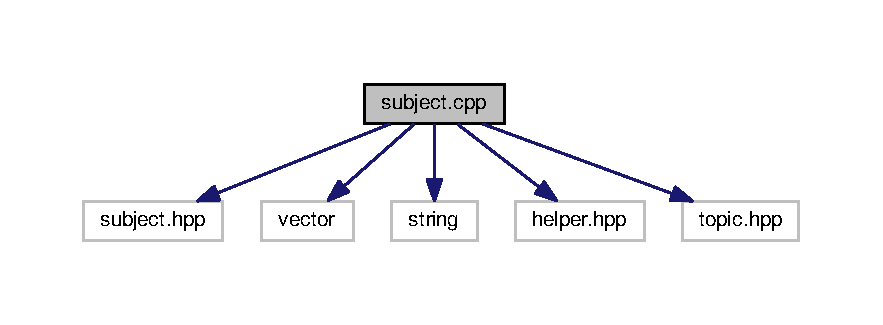
\includegraphics[width=350pt]{subject_8cpp__incl}
\end{center}
\end{figure}

\hypertarget{subject_8hpp}{}\section{subject.\+hpp File Reference}
\label{subject_8hpp}\index{subject.\+hpp@{subject.\+hpp}}
{\ttfamily \#include $<$string$>$}\newline
{\ttfamily \#include $<$vector$>$}\newline
{\ttfamily \#include \char`\"{}topic.\+hpp\char`\"{}}\newline
{\ttfamily \#include \char`\"{}quiz.\+hpp\char`\"{}}\newline
\subsection*{Classes}
\begin{DoxyCompactItemize}
\item 
class \hyperlink{class_subject}{Subject}
\begin{DoxyCompactList}\small\item\em Responsavel por adicionar novos topicos e mostrar topicos existentes de uma disciplina. \end{DoxyCompactList}\end{DoxyCompactItemize}

\hypertarget{topic_8cpp}{}\section{topic.\+cpp File Reference}
\label{topic_8cpp}\index{topic.\+cpp@{topic.\+cpp}}
{\ttfamily \#include \char`\"{}topic.\+hpp\char`\"{}}\\*
{\ttfamily \#include $<$vector$>$}\\*
{\ttfamily \#include \char`\"{}helper.\+hpp\char`\"{}}\\*
{\ttfamily \#include \char`\"{}quiz.\+hpp\char`\"{}}\\*
Include dependency graph for topic.\+cpp\+:
\nopagebreak
\begin{figure}[H]
\begin{center}
\leavevmode
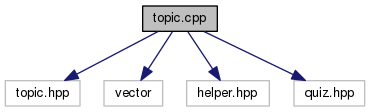
\includegraphics[width=350pt]{topic_8cpp__incl}
\end{center}
\end{figure}

\hypertarget{topic_8hpp}{}\section{topic.\+hpp File Reference}
\label{topic_8hpp}\index{topic.\+hpp@{topic.\+hpp}}
{\ttfamily \#include \char`\"{}quiz.\+hpp\char`\"{}}\newline
{\ttfamily \#include $<$string$>$}\newline
{\ttfamily \#include $<$vector$>$}\newline
\subsection*{Classes}
\begin{DoxyCompactItemize}
\item 
class \hyperlink{class_topic}{Topic}
\begin{DoxyCompactList}\small\item\em \hyperlink{class_topic}{Topic} eh a classe dos topicos de cada disciplina. \end{DoxyCompactList}\end{DoxyCompactItemize}

\hypertarget{user_8cpp}{}\section{user.\+cpp File Reference}
\label{user_8cpp}\index{user.\+cpp@{user.\+cpp}}
{\ttfamily \#include \char`\"{}user.\+hpp\char`\"{}}\\*
{\ttfamily \#include $<$string$>$}\\*
{\ttfamily \#include $<$vector$>$}\\*
{\ttfamily \#include $<$algorithm$>$}\\*
{\ttfamily \#include \char`\"{}helper.\+hpp\char`\"{}}\\*
{\ttfamily \#include \char`\"{}subject.\+hpp\char`\"{}}\\*
{\ttfamily \#include \char`\"{}topic.\+hpp\char`\"{}}\\*
{\ttfamily \#include \char`\"{}quiz.\+hpp\char`\"{}}\\*
Include dependency graph for user.\+cpp\+:
\nopagebreak
\begin{figure}[H]
\begin{center}
\leavevmode
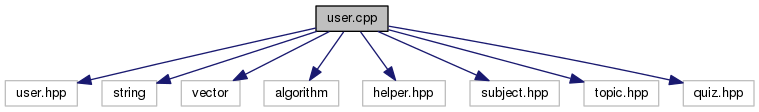
\includegraphics[width=350pt]{user_8cpp__incl}
\end{center}
\end{figure}

\hypertarget{user_8hpp}{}\section{user.\+hpp File Reference}
\label{user_8hpp}\index{user.\+hpp@{user.\+hpp}}
{\ttfamily \#include $<$string$>$}\newline
{\ttfamily \#include $<$vector$>$}\newline
{\ttfamily \#include \char`\"{}subject.\+hpp\char`\"{}}\newline
{\ttfamily \#include \char`\"{}topic.\+hpp\char`\"{}}\newline
{\ttfamily \#include \char`\"{}quiz.\+hpp\char`\"{}}\newline
\subsection*{Classes}
\begin{DoxyCompactItemize}
\item 
class \hyperlink{class_user}{User}
\begin{DoxyCompactList}\small\item\em Po, tem que funfar em Windows tmb ne. \end{DoxyCompactList}\end{DoxyCompactItemize}
\subsection*{Typedefs}
\begin{DoxyCompactItemize}
\item 
using \hyperlink{user_8hpp_a69aa29b598b851b0640aa225a9e5d61d}{uint} = unsigned int
\end{DoxyCompactItemize}


\subsection{Typedef Documentation}
\mbox{\Hypertarget{user_8hpp_a69aa29b598b851b0640aa225a9e5d61d}\label{user_8hpp_a69aa29b598b851b0640aa225a9e5d61d}} 
\index{user.\+hpp@{user.\+hpp}!uint@{uint}}
\index{uint@{uint}!user.\+hpp@{user.\+hpp}}
\subsubsection{\texorpdfstring{uint}{uint}}
{\footnotesize\ttfamily using \hyperlink{user_8hpp_a69aa29b598b851b0640aa225a9e5d61d}{uint} =  unsigned int}



Definition at line 20 of file user.\+hpp.


%--- End generated contents ---

% Index
\backmatter
\newpage
\phantomsection
\clearemptydoublepage
\addcontentsline{toc}{chapter}{Index}
\printindex

\end{document}
